\documentclass[11pt]{aucklandthesis}
%
% This is a template for University of Auckland theses.
%
% Written by Alistair Kwan, June 2016
% 
%
% Options:
%	10pt, 11pt, 12pt: size of main text
% 	examcopy: asserts confidentiality for examination copies
%	partial: thesis partial fulfils degree requirements
%	singlespace, onehalfspace, doublespace: line spacing
%	oneside: format for single-sided printing
%	draft: adds 'draft' and date to footer
%

%
% Add, delete or un-comment packages below as required.
%

\usepackage[utf8]{inputenc}
\usepackage[T1]{fontenc}
\usepackage{natbib}

\usepackage{graphicx} % for inserting graphics files
\usepackage{appendix} % for appendices

\usepackage{hyperref} % for formatting web addresses and other URLs
\usepackage{csquotes} % for block quotes

\usepackage{lscape} %for landscape/rotated figures and tables

\usepackage{rotating}

\usepackage{afterpage}

%\urlstyle{same} % try also tt, sf if this option doesn't produce clear enough output

% Readability options
%
%\usepackage{booktabs} % for table rules
%\usepackage{microtype} % for improved justification

% Typeface options — choose one if desired
% or choose a different typeface to accommmodate character sets
% as needed for East Asian and other languages.
%
% Consider compiling using the XeLaTeX engine if you have more extreme
% typeface needs, e.g. for multiple languages, or a need for symbols particular
% to a typeface.
%
% See also the LaTeX Symbols List at
% https://http://www.ctan.org/pkg/comprehensive
%
%\usepackage{mathptmx} % Times New Roman, including mathematics
%\usepackage{mathpazo} % Palatino with mathematics support
%\usepackage{fourier} % Utopia, a serif typeface with Fourier mathematics
%\usepackage{gentium} % a contemporary serif typeface
%\usepackage{libertine} % a softer-feeling serif typeface; also installs sans-serif font Biolinum
%\usepackage{fouriernc} % Century Schoolbook with Fourier maths
%\usepackage{mathpple} % Palatino with Fourier maths


% To set the sans serif font (for \sffamily):
%\usepackage[scaled]{helvet} % Nimbus, like Helvetica
%\usepackage{universalis} % Universalis
%\usepackage{avant} % URW Gothic, like Avant Garde
%\usepackage{PTSansNarrow}
%\usepackage{AlegreyaSans} % Alegreya Sans

% To set the mathematics font:
%\usepackage{eulervm} % Euler, based on a Zapf design

% To set the (usually monospaced) typewriter font:
%\usepackage[ttdefault=true]{AnonymousPro}
%\usepackage[scaled]{beramono}
%\usepackage{inconsolata}
%\usepackage{sourcecodepro}

%\usepackage{cjk} % for Chinese, Japanese, Korean

%\usepackage{tabularx} % For easier table formatting.

%\usepackage[nottoc]{tocbibind} % Controls the table of contents
%   nottoc: don't list table of contents inside itself
%   section: go as far as section-level headings

% Automated bibliography
%
%\usepackage[
%	style=authortitle, 
%	citestyle=authortitle,
%	backend=biber
%	]
%	{biblatex}
%bibliography{bibliography1.bib, bibliography2.bib} % Specify bibliography files 

\begin{document}

% ====================================================
%
% FRONTMATTER
%
% Arabic pagination, starting with the title page
% which is counted but not numbered
%
% ====================================================

% Specify the title page content
\title{Understanding Participation in Science Education in New Zealand}
\subtitle{A Mixed Methods, Bourdieusian Approach}
\author{Steven Martin Turnbull}
\degreesought{Doctor of Philosophy} 
\degreediscipline{Education}
\degreecompletionyear{2020}

% Print the title page
\maketitle

% Abstract, up to 350 words
\chapter*{Abstract}
Words gonna go here
 % it's in a separate file
\addcontentsline{toc}{chapter}{Abstract}
% Dedication (optional)
\thesisdedication{Dedicated to grandma, and to grammar.}

% Preface and/or acknowledgements (optional)
\chapter*{Acknowledgements}

\addcontentsline{toc}{chapter}{Preface and Acknowledgements}
% it's in a separate file

% Contents, lists of tables and figures
\settocdepth{section} %choose chapter, section, subsection
\cleardoublepage\tableofcontents
%\cleardoublepage\listoffigures
%\cleardoublepage\listoftables

% Glossary (optional)
\chapter*{Glossary}.
\addcontentsline{toc}{chapter}{Glossary}
% ====================================================
%
% MAINMATTER
%
% Include external chapter files here using
% the \input{} command
%
% If you run out of memory during compilation,
% switch some or all chapters to \include{} instead of \input{}, 
% but watch out for pagination problems.
%
% ====================================================

\chapter{Introduction}

\section{Understanding Participation in Science Education}
There has been an increasing drive to address issues surrounding equity and access in science education. Much research has shown that educational interests in science and technology have declined over time \citep{OECD2006}. In addition, there tends to be uneven levels of interests and retention in science and technology across various demographic characteristics, including ethnicity, gender \citep{cheryan2017some,su2015all}, and Socio-Economic Status (SES). Across the world, there is increasing demand to address these inequities. In New Zealand, the need to address inequities are particularly salient for government. As outlined in the Child Youth and Wellbeing Strategy \citep{wellbeing2019}, it is important that young people are not only learning and developing, but they are doing so in a way that ensures that they are happy and healthy. Te Tiriti o Waitangi (The Treaty of Waitangi) also sets out a requirement for intergenerational inequities to be addressed regarding M\={a}ori \citep{treatywaitangi}, the indigenous population of New Zealand who still suffer from the impact of colonisation. When applied to the field of science education, researchers and policy makers are thus charged with understanding and addressing disparities related to science participation, achievement, and interests. 

Research into inequities in STEM often focuses on one aspect of an individuals identity, with the cost of sacrificing an intersectional perspective that can provide more understanding of each individual's unique life circumstances. Forsaking an intersectional approach can lead to the life experiences of certain groups going unreported and unheard. There is an increasing wealth of literature detailing gender disparities in STEM interests and outcomes \citep{Sue2009,wang2017gender}, but there are relatively fewer studies that explore intersections with ethnicity \citep{fouad2017scct,grossman2014perceived}, and even fewer still that investigate the intersections between gender, ethnicity and social class \citep{archer2013aspires}. Many researchers are now advocating for intersectional approaches to understand student experiences in STEM and at university \citep{jury2017experience}. It is also important to consider that, while it can be relatively simple to operationalise gender and ethnicity (i.e., through self-identification), social class is a more difficult construct to define and operationalise. Socio-economic status is the most commonly used indicator of social class, but as argued by \cite{rutkowski2013measuring}, a `one size fits all' approach to SES can be criticized for neglecting cross-country and cross-cultural differences. This argument can be extended further by exploring how social class relates to a students specific field of study or career intention. While having parents with highly paid jobs has been shown to be beneficial for students across different contexts, research has also shown that parents employment is linked to domain-specific preferences in education. Children who have parents who work as scientists are more likely to grow up study science themselves \cite{moakler2014college}, with this being especially true in physics \citep{upshot}. Recent research in science education has applied Pierre Bourdieu's sociological theory of taste to operationalise social class in terms of cultural and social capital \citep{Archer_2015}. These concepts not only provide a method of conceptualising social class that realises the social, cultural, and historical contexts in which individuals are placed, but it also provides an underlying theoretical framework that details how social class intersects with other aspects of identity (i.e., across axes of ethnicity and gender). 

As noted by theorists, capital by its very nature is not distributed evenly across society. Students from less affluent backgrounds tend to have poorer educational outcomes \cite{May_2016}, and are less likely to realise tertiary education goals \cite{reynolds2011change}. Students who do not have parents or family members who attended university face additional challenges in adapting to life at university. 

In New Zealand access to capital is disproportionately distributed across ethnic groups. M\={a}ori and Pasifika students are over represented in low SES areas (an ongoing consequence of New Zealand's colonial history), subjected to everyday racism and discrimination \citep{mayeda2014you}, and are the subject of lower academic expectations from teachers \citep{turner2015teacher}. Given these findings, it is not surprising that research shows that M\={a}ori and Pasifika students are less likely to be retained in university study, with especially true with regards to scientific disciplines \cite{EducationCounts_2019}. 

The current study combines the theoretical framework of Bourdieu with an intersectional approach in order to understand students' experiences of university science education. The goal of this research is to explore how an individuals social location relates to access to resources and relationships (capital), and how this relates to students' identity within the field of university science education. The following sections will define the concepts of cultural and social capital, and summarise the relevance of these concepts to university science education. It will then outline the concept of habitus, the ``internal system of dispositions'' that Bourdieu saw as the mediator between external societal structures and individual agency. It is through habitus that students internalise the world around them and judge what is `for them', where their interests lie, and what their lifestyle choices are. 

\section{Understanding the Structure of this Thesis}
The goal of my thesis is to provide an in depth understanding of science education in New Zealand, with the specific aims of answering three broad research questions.  I seek to understand \textit{what} science participation looks like in New Zealand, \textit{why} is it the case, and \textit{how} we may improve equitable outcomes. The thesis itself is a combination of articles that have been submitting to journals and chapters written specifically for the thesis. As a result, some content may be repeated. Given the thesis was written over the period of three years, it is also possible that my understanding of Bourdieu's theory will be more developed in chapters written recently compared to older chapters. Each chapter will include a preamble which will place the following chapter in the context of which is was originally written, and in the context of the overall goals of the thesis. The following section provides an overview of how each one of my chapters fits within the goals of the thesis. 

Firstly, I seek to understand \textit{what} science participation looks like in New Zealand. Chapters 2 and 3 discuss the analysis of two big administrative data sets. The first data set was obtained through the Integrated Data Infrastructure (IDI) and represents all students from 2010 to 2016 studying Level 3 STEM standards in New Zealand high schools, while the second data set represents students studying who studied physics at undergraduate level from 2010 to 2016. In both of these chapters I employ network analysis as a method of untangling trends in complex data. For the purposes of this thesis, it was my intention for someone unfamiliar with network analysis to be able to understand the procedures behind the analysis, and more importantly, why it was used. 

Whilst both Chapters 2 and 3 detail \textit{what} science participation looks like in New Zealand, Chapter 3 also begins to delve into possible reasons for \textit{why} we see disparities in science participation. In Bourdieusian terms, Chapters 2 and 3 explain the state of the field of science education. Chapter 3 introduces Bourdieu's other concepts of capital and habitus as concepts that may explain \textit{why} the field is structured as it is, and the following chapters build on this model. Chapter 4 details the results of a survey that explored the relationships between forms of science-related capital and students' self-concept of science --- which I argue is the aspect of habitus that can be scrutinised through introspection. Chapter 5 details the development of a new conceptual model. This new model expands on the original Bourdieusian model outlined in Chapter 3, with the aim of highlighting the importance of social capital in particular, and the reciprocal relationship shared between capital and habitus. 

Following the development of the new conceptual model of capital and habitus in Chapter 5, Chapter 6 seeks to put the lived experiences of science students to the model. These students, purposefully sampled from the results of the survey discussed in Chapter 4, detail a range of different experiences. Through analysis of this qualitative data I try to unpack how science participation may be influenced by social location. 

After providing answers to the \textit{what} (Chapters 2 and 3) and the \textit{why} (Chapters 3 to 6), the final goal of the thesis is to suggest a \textit{how}: how can we improve the field of science education so that it is more equitable. Chapter 7 draws upon the conceptual model outlined in Chapter 5, the qualitative data detailed in Chapter 6, and the findings of previous research, to suggest opportunities for intervention that may make the field of science education more equitable. 



\chapter{Understanding Science Participation in New Zealand}
\chapter[Bourdieu, Networks, and Movements][]{Bourdieu, networks, and movements: Using the concepts of habitus, field and capital to understand a network analysis of gender differences in undergraduate physics}

\section{Preamble}
The following work was published in PLoS ONE on the 2nd of September 2019 (https://journals.plos.org/plosone/article?id=10.1371/journal.pone.0222357). Coauthors included Kirsten Locke\textsuperscript{1,2}, Fr\'ed\'erique Vanholsbeeck \textsuperscript{3,4}, and 
Dion R. J. O'Neale\textsuperscript{2,3}
\footnote{\textbf{1} Critical Studies in Education, Faculty of Education and Social Work, University of Auckland, Auckland, New Zealand
\\
\textbf{2} Te P\={u}naha Matatini, University of Auckland, Auckland, New Zealand
\\
\textbf{3} Department of Physics, University of Auckland, Auckland, New Zealand
\\
\textbf{4} The Dodd-Walls Centre, University of Auckland, Auckland, New Zealand}. 

This article was written in the first year of my PhD, and serves as the basis for the whole thesis. It provides the bridge between understanding \textit{what} science education looks like in terms of broad patterns of enrolments, and understanding \textit{why} these patterns exist. The methods follow on from Chapter 2, in that I employ the same network analysis procedures only on a different dataset. Instead of NCEA data, I now explore patterns in course enrolment data for undergraduate physics students at the University of Auckland. I also frame this analysis in the sociological theory of Pierre Bourdieu using a simple model of his concepts of capital, habitus, and field. 

\section{Abstract}
Current trends suggest that significant gender disparities exist within Science, Technology, Engineering, and Mathematics (STEM) education at university, with female students being underrepresented in physics, but more equally represented in life sciences (e.g., biology, medicine). To understand these trends, it is important to consider the context in which students make decisions about which university courses to enrol in. The current study seeks to investigate gender differences in STEM through a unique approach that combines network analysis of student enrollment data with an interpretive lens based on the sociological theory of Pierre Bourdieu. We generate a network of courses taken by around 9000 undergraduate physics students (from 2009 to 2014) to quantify Bourdieu's concept of field. We identify the fields in which physics students participate by constructing a weighted co-enrollment network and finding communities within it. We then use odds ratios to report gender differences in transverse movements between different academic fields, and non-parametric tests to assess gender differences in vertical movements (changes in students' achievement rankings within a field). Odds ratios comparing the likelihood of progression from one field to another indicate that female students were more likely to make transverse movements into life science fields. We also found that university physics did a poor job in attracting high achieving students, and especially high achieving female students. Of the students who did choose to study physics at university, low and middle achieving female high school students were more likely to decrease their relative rank in their first year compared to their male counterparts. Low achieving female students were also less likely to continue with physics after their first year compared to their male counterparts. Results and implications are discussed in the context of Bourdieu's theory, and previous research. We argue that in order to remove constraints on female students' study choices, the field of physics needs to provide a culture in which all students feel like they belong.



\section{Introduction}
Historically, women have been underrepresented in Science, Technology, Engineering and Mathematics (STEM) disciplines. This is a concerning issue today internationally, and at all stages of higher education.\cite{Abraham_2014,Stevanovic_2013,Smith_2011} More recent studies indicate specific gender disparities exist within the sub-fields that comprise STEM.\cite{mullis2016timss} Female students tend to be underrepresented in physics in higher education, and this is evidenced by research from the United States\cite{NSF, Cunningham_2015,Kost_Smith_2010,Heilbronner_2012}, Europe\cite{Huyer2007, Stevanovic_2013, InstituteofPhysics_2012, InstituteofPhysics_2013, Smith_2011}, Asia-Pacific regions\cite{EducationCounts_2016a, Kennedy_2014} and Africa.\cite{Semela_2010} In contrast, the same research shows that the life science subjects (biology and medicine) tend to have more of a gender balance. Further studies have shown that gender disparities exist not only in subject participation, but in the levels of confidence that students have across subjects. Female students tend to be less confident than their male peers in physics\cite{kelly2016social, Hofer_2016} and calculus\cite{Ellis_2016}, even after controlling for actual academic achievement.\cite{marshman2018female} Why do we see gender differences in the physical and mathematical science subjects, but not the life science subjects? Much research has been dedicated to understanding the extent, causes, and possible solutions to this issue.\cite{cheryan2017some,Brewe_2016, Blickenstaff_2005}

The current study investigates the outcomes for male and female physics students at the University of Auckland (UoA) --- the largest university in New Zealand. We adopt a unique approach, by combining quantitative network analysis with a research framework based on Pierre Bourdieu's sociological theory.\cite{Bourdieu1984} Whilst we argue that these two approaches can provide a detailed understanding of gender disparities in student enrollment patterns, there is a lack of research in this area (for examples of how network analysis and Bourdieu have been previously used together, see the work of de Nooy\cite{de2003fields}, and Bottero and Crossley\cite{bottero2011worlds}). We combine these approaches by using network analysis to provide a representation of Bourdieu's concept of field, with an emphasis on his ideas of transverse and vertical movements (students moving from one field to another, and moving upwards and downwards in achievement rankings in a field). In order to avoid misinterpretation of Bourdieu's theory, which is easily done when ``bits and pieces'' of it are used\cite{Bourdieu1992}, we combine our representation of field with Bourdieu's concepts of habitus and capital. We argue that network analysis can bring to light the complex patterns of students' subject enrollment, whilst Bourdieu's theory offers a rich theoretical framework to explain these patterns. We place the findings of our network analysis in a broad socio-cultural context that brings to light the complex interactions between society, gender and subject discipline. To avoid confusion, the following sections will use `field' as a technical term referring to the Bourdieu's definition (which will be explained in more detail in the next section), and `discipline' as a non-technical term that describes the different STEM domains. 

We begin by introducing a simple model of Bourdieu's theory, using the field of science education to illustrate its concepts. We then add to this outline of theory by building our method of network analysis into Bourdieu's theory. More specifically, we describe how network analysis of student enrollment data can provide a representation of field. Exploring the properties of this network structure allows us to understand gender differences in the movements students make within and across fields. According to Bourdieu\cite{Bourdieu1984}: 
\begin{quote}
    The social space, being structured in two dimensions (overall capital volume and dominant/dominated capital) allows two types of movement... vertical movements, upwards or downwards in the same vertical sector, that is in the same field... and transverse movements, from one field to another, which may occur either horizontally or between different levels.
\end{quote} In science education, individual's may move from one field to another (i.e., from physics to life science), but also upwards and downwards in achievement rankings in the field. We use these concepts of movements to guide our investigation. We seek to understand whether there are gender differences in the number of students moving from physics to other fields, and also in the changes in achievement rankings of students in physics. We close this article with a discussion of our results in the broader context of previous research and Bourdieu's concepts of capital and habitus. 

\section{Theoretical Framework}
The metaphor of the leaky pipeline is often used to describe the attrition of women from physics\cite{Huyer2007, Schiebinger_2001}, in that women are more likely to drop out with each transition between key stages of education (particularly secondary school to university). This metaphor can be criticized for not only stigmatizing individuals that drop out of the pipeline, but for also being too simplistic.\cite{Cannady2014} It is important to emphasize contextual factors, such as the presence of gender-stereotypes\cite{Nosek_2009} (e.g., men study science, women study humanities) that impact on the decisions that students make. It is also important to consider the complex nature of students' enrollment patterns; in reality a student's journey through university study follows a complex network of unique pipes, rather than a singular pipeline. The current study employs a research framework that builds on the limitations of the leaky pipeline. We seek to place our results in a wider socio-cultural context, by harnessing a research framework adapted from the work of Pierre Bourdieu\cite{Bourdieu1984} (see Fig~\ref{Fig1}). We employ Bourdieu's concepts of capital, habitus and field to interpret our findings, and place them in the context of previous studies that have investigated gender differences in STEM subject selection. 

\begin{figure}[!ht]
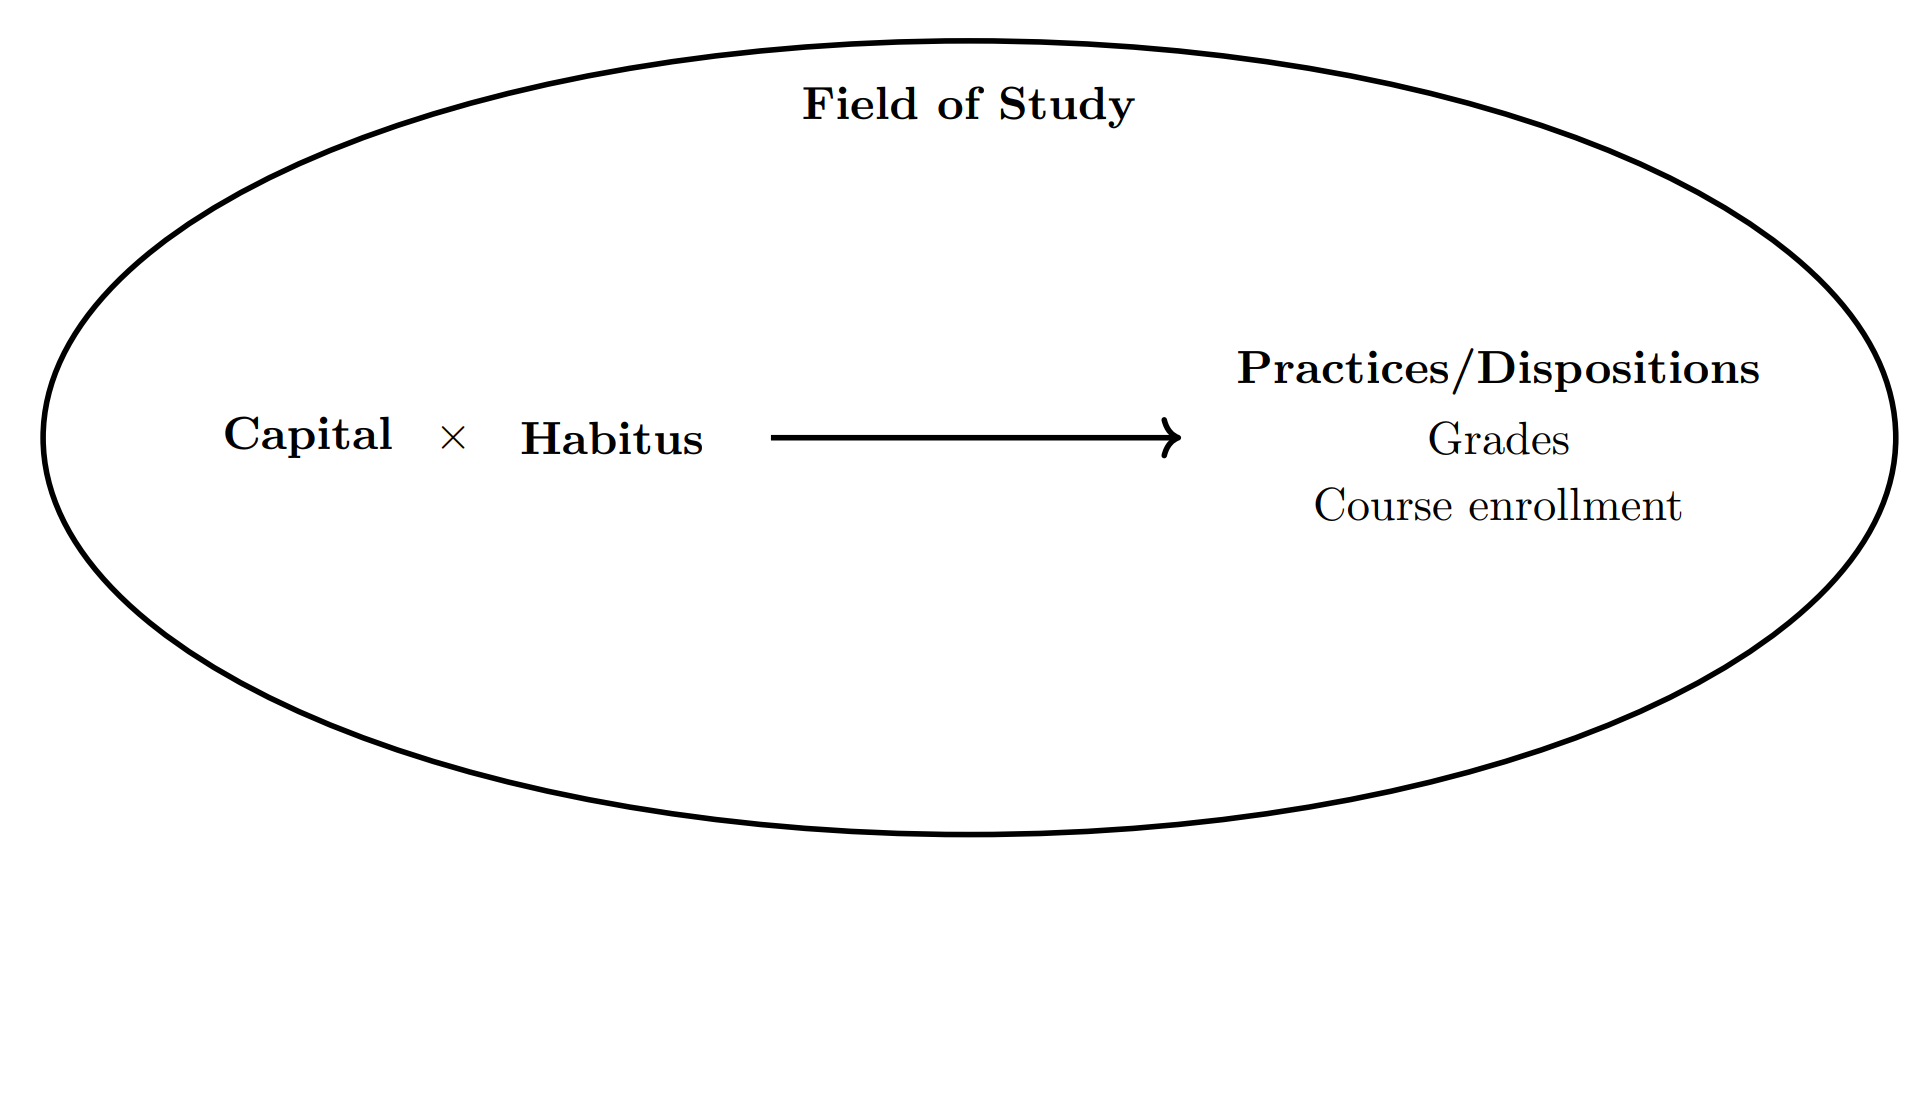
\includegraphics[width = \linewidth]{C3 - Bourdieu Networks/C3 - Fig1.png}
\begin{center}
\end{center}
\caption{\textbf{Simplified Bourdieusian Theoretical Model.\newline}
The Bourdieusian framework used in the current study is adapted from the original model outlined by Bourdieu\cite{Bourdieu1984} and the work of Archer and colleagues.\cite{Archer2012,Archer2014, Archer_2015} A student's habitus interacts with their acquired level of capital (in particular science-related capital) to generate a student's practices (behaviours, grades etc.) and their dispositions towards the field. A student's habitus, a matrix of internal dispositions\cite{Reay2004}, is formed in relation to the specific socio-cultural and historical context of a field. A student who is positively predisposed to study in a scientific field, whilst also having access to various forms of science-related capital, will likely achieve higher grades in that field and aspire to study in that field in the future. A student who encounters bad experiences in the field will likely be dissuaded from future study via their habitus (`this discipline is not for me').}
\label{Fig1} 
\end{figure}

The following sections will outline Bourdieu's concepts of field, capital and habitus. We apply these concepts to a host of previous research regarding gender disparities in science to outline the socio-cultural context in which students are placed. More specifically, we outline research that describes the state of the field of physics and the distribution of capital within the field of physics. We then discuss the interaction of capital with habitus --- the system of dispositions that is formed in relation to the field. We describe how the ``smog of bias''\cite{Kost_Smith_2010} that targets women in physics may impact on habitus, and thus practices within the field, such as choosing to discontinue physics study. 

\subsection{Field}
For Bourdieu, the world is separated into a collection of different fields.\cite{Bourdieu1984} A field can be considered as a system of social locations, where each individual is objectively ranked by the resources (capital) they have relative to others. For example, in the field of tertiary science education, a lecturer ranks higher than a student, whilst a high achieving student ranks higher than a low achieving student. To begin to the understand the hierarchical nature of a field, we must first understand the concept of \textit{capital}. Originally conceived within economics, capital was defined by Adam Smith (in 1887) as ``That part [of a person's wealth] that he expects to provide [them] with \textellipsis income\textellipsis''.\cite{Smith_1887} Bourdieu interpreted capital as a legitimate, valuable and exchangeable resource that individuals can use to gain advantage in society.\cite{Bourdieu_1986}

Therefore, the rankings are determined by how we define what is valuable and legitimate in the field. The practices of an individual within the field, which are guided by the individual's internal dispositions (habitus), are judged by criteria internal to the domain of activity.\cite{hilgers2014introduction} Individuals with a high volume of valued capital will hold power within the field. For example, high achieving students have high volumes of capital in the field due to their course grades (a signal of success), whilst lecturers and researchers have a greater volume of capital in the form of qualifications and research experience. In the field of tertiary science education, lecturers and researchers sit at the top of the hierarchy, and decide what kinds of capital are valued or devalued (e.g., professors often decide the course content and manner of teaching for undergraduate students at university). We will discuss Bourdieu's conceptualization of capital and the way it can inform gender equity research in the following section. Before then, we will outline a brief description of how the field of physics is structured from an objective point of view in relation to gender.

The numbers of male and female students holding qualification in the different science disciplines can provide an objective, surface level understanding of the structure of the field. In the United States, only around 20\% of students studying physics at bachelors, masters or doctorate level in 2014 were female.\cite{NSF} This contrasts with biology, where around 50-60\% of students studying at bachelors, masters or doctorate level were female.\cite{NSF} Similar gender disparities in physics enrollments have been found in the European\cite{InstituteofPhysics_2012,InstituteofPhysics_2013, Stevanovic_2013} and Asia-Pacific regions.\cite{Abraham_2014, Kennedy_2014} Data from UNESCO  shows that, in Europe in 2007, around 71\% of tertiary health and welfare students were female, whilst this figure was 39\% for natural and physical science (biology, physics, chemistry).\cite{Huyer2007} 

Reports from New Zealand in 2017 show that, overall, secondary school science had a balanced gender-ratio of year 13 (i.e. final year of high-school) students.\cite{EducationCounts_2016a} However, male students dominated physics and mathematics from year 11 to year 13 at secondary school, with this trend being reflected at university level.\cite{EducationCounts_2016a} Across the same school years, biology and human anatomy tended to have more female students than male students. Looking at tertiary science education (i.e. university undergraduate and post-graduate levels), these gender disparities were maintained.\cite{EducationCounts_2016a} Other data from New Zealand in 2017 shows that female students were slightly less well represented among bachelor students studying physics and mathematics (43\% and 46\% respectively).\cite{EducationCounts_2016b} At the same level, female students tended to be over-represented in biology and health (67\% and 74\% respectively).\cite{EducationCounts_2016b} Approximately 25\% of doctoral students in physics and astronomy and 44\% of students in mathematics were female, while female students comprised 53\% of students studying biology and 69\% of those studying health. Beyond post-graduate level study, the representation of women in New Zealand professorial roles and leadership positions in physics is particularly poor. For example a report by the New Zealand Association for Women in the Sciences, published in 2011, noted that women were only $29\%$ of workers employed in physics related roles (New Zealand census data); approximately $10\%$ of research active employees in physics at New Zealand universities; and had no representation on the main grant review panel for physics related fundamental research in New Zealand (the Marsden fund).\cite{Bray_2011}

The above outlines clear evidence of gender disparities in the field of science, internationally and in New Zealand specifically. Whilst useful, these figures only provide a static, surface-level understanding of what is happening in the field of science education. As shown in Fig \ref{Fig1}, the practices and behaviours represented in the field (such as enrollment patterns) are generated through the interaction of capital (resources) and habitus (internal dispositions). We will now visit these two concepts, applying them to previous research, to understand why gender disparities in science education are common.   

\subsection{Capital}
The objective rankings within a field are defined by the distribution of capital, and this can be used to inform gender equity research in science.\cite{Kelly_1985} Different fields have different forms of logic as to what forms of capital are of value. Using a basic example, a science qualification is worth more in the field of science than in other academic fields. Capital is complex and may take many forms, each of which may be valued differently depending on the dominant logic of the field. According to Bourdieu\cite{Bourdieu_1986}, capital has four forms: economic (e.g., financial resources), cultural (non-financial assets, such as physical appearance, spoken language, academic achievement), social (e.g., an individual's social network), and symbolic (prestige and recognition, such as awards). Individuals who begin their life with more capital, be that through inheritance or immediate exposure to the dominant culture, will be more able to gain personal and social advantages. For example, a student who is born into a family that speaks the dominant language of an educational institution may find it easier to learn, and a student with greater economic wealth may be more able to afford the costs associated with tertiary study (e.g., tuition fees, relocation, travel). The value of capital is not solely determined by form, but also by factors such as the manner of acquisition, and the personal characteristics of the owner. Issues emerge when an individual's capital is devalued unjustly by the `rules' operating in the field. For example, international research has shown that female physicists tend to receive fewer opportunities and career enhancing resources compared to objectively equal male physicists.\cite{Ivie_2013} Previous research of tertiary students suggests that female students may be more likely to discontinue physics education, regardless of performance.\cite{Ellis_2016,Ost_2010} Since disparities in enrollment still exist even after controlling for academic achievement, it is likely that capital is not the dominant factor in driving gender differences in physics education outcomes. Research does suggest, however, that the gender disparities in physics enrollments can be understood in terms of students' identity\cite{Brown2010,Hazari_2010,Hazari2013,Brewe_2016,Hazari2017} and self-confidence\cite{Litzler2014,Concannon2009,Sharma_2011,Beth_Kurtz_Costes_2008,Sawtelle_2012} -- factors that can be tied to Bourdieu's concept of habitus.

\subsection{Habitus}
Capital, in its various forms, interacts with habitus (Fig~\ref{Fig1}); a construct defined by Bourdieu as a ``system of dispositions''\cite{Bourdieu1984} formed in relation to a field. Whilst capital is what determines one's position within the field, habitus is what determines one's disposition towards it.\cite{Bourdieu1992} An individual's habitus is the internalization of the socio-cultural and historical context of a field, and it operates ``below the level of consciousness and language''.\cite{Bourdieu1984} Nash\cite{Nash1999} understood habitus as ``a system of schemes of perception and discrimination embodied as dispositions reflecting the entire history of the group and acquired through the formative experiences of childhood''. In simple terms, habitus is what we use to determine whether the field is something we are interested in, based on evidence present in the environment. Whilst habitus is generally formed during childhood within the family\cite{Dimaggio1982}, it is continually reconstructed and transformed as an individual operates in society. For example, a student who grows up in a family that places high value on science may share the same disposition.\cite{archer2013aspires} However, an individual may not choose to pursue science when faced with evidence that the field is not for them (for example, receiving poor grades, being treated poorly, lack of role models). Based on this internal matrix of dispositions, an individual's lifestyle practices are generated. According to Bourdieu, the collection of each individual lifestyle produced by habitus then constitutes the ``represented social world''\cite{Bourdieu1984} --- the way that things appear to be. As the representation of the social world also influences the formation of habitus, the world and habitus share a reciprocal relationship. This relationship facilitates the cultural reproduction of inequity over time. 

Habitus can be used as a concept to explain the gender disparities in science enrollments. Based on what they see in their represented social world, students will ``[refuse] what they are refused (`that's not for the likes of us'), [adjust] their expectations to their chances, [and define] themselves as the established order defines them.''.\cite{Bourdieu1984} Based on what students see in their environment, they will make decisions on what they feel is a realistic study choice. Archer and colleagues explain this idea further: ``social axes of `race'/ethnicity, social class, and gender all contribute to shaping what an individual perceives to be possible and desirable.''.\cite{Archer_2012} The manner by which students perceive the different scientific disciplines, as they are represented in society, likely plays an important role in influencing their desire to study those disciplines. 
A wealth of research has outlined the various ways that women are subjugated in certain STEM disciplines, especially physics, with the culmination of these factors being referred to as ``the smog of bias''\cite{Kost_Smith_2010} or the ``gender filter''.\cite{Blickenstaff_2005} No single factor can sufficiently explain why women are less likely to pursue physics\cite{Kost_Smith_2010}, but a host of factors are likely to interact and impact on the dispositions students hold (habitus). Due to the pervasiveness of these various factors across society, habitus can take on a collective quality where individuals tend to hold stereotypical views on what is expected for members of different groups. To provide a simple example, research across 34 countries has shown that science tends to be implicitly associated with men more than with women, and that this level of gender bias predicts gender differences in science performance.\cite{Nosek_2009} As outlined by Bourdieu, an objective class of individuals can be considered the ``the set of agents who are placed in homogenous conditions of existence imposing homogenous conditionings and producing homogenous systems of dispositions capable of generating similar practices''\cite{Bourdieu1984}. In more basic terms, individuals who share similar backgrounds and characteristics will have a similar habitus, and this may predispose them to behave in similar ways.\cite{Reay2004}

Every student holds beliefs about their possible educational paths. However, these beliefs are informed, implicitly and explicitly, by evidence in the environment. When deciding on whether to pursue physics, a student may ask: how are people like me treated in physics? Do people see me as a physicist? How many people like me study physics? Whilst we acknowledge that this is not an exhaustive list of reasons why students study physics, the answers to these questions are likely skewed to favour male students over female students. A study by Ong\cite{ong2005body} highlighted the incongruence felt by minority female physics students as they studied physics, where their competence was unfairly questioned because their `bodies did not fit' with the stereotypical depiction of the white male scientist. Similarly, studies have found that women are more likely to be viewed as incompetent, controlling for confounding variables other than gender, by scientists (including physicists) looking to hire a laboratory manager\cite{Moss_2012}, or by students evaluating their physics teacher.\cite{Potvin_2016} Similarly, women rated as more feminine are less likely to be judged as a scientist.\cite{Banchefsky2016} The pervasive nature of the ``smog of bias''\cite{Kost_Smith_2010} in physics offers the `homogenous conditions of existence' that may result in a gendered habitus in physics: one that sees physics as unwelcoming for female students. This is likely to explain why studies tend to find that female students are more interested in life science subjects\cite{Buccheri_2011} and male students are more likely to be interested in physics, engineering and mathematics.\cite{Su_2009, B_E_2013, Cunningham_2015} It is important to note here that the opposite is not true --- there is a lack of evidence to suggest that male students are unfairly judged as incompetent or feel unwelcome in the life sciences and therefore choose physical science subjects.  

Evidence suggests that the gender differences in subject interest may not be present in early childhood, but emerge by the end of secondary school.\cite{Baram_Tsabari_2010} This lends credence to the idea that habitus is formulated over time; as individuals become increasingly aware of societal norms, their interests align with what (through their habitus) seems like a realistic study choice. These stereotypical gender preferences may persist when it comes to the types of science-related career that secondary school students aim for\cite{Kj_rnsli_2011}, and students' choice of STEM major at university.\cite{Bottia_2015, Sadler_2012} At university level, gender disparities may even widen further; a study of physics students at a university in the United States found that female students are more likely to see their interest in physics diminish during introductory physics.\cite{Kost_Smith_2010}

\subsection{The Current Study}

The current study was motivated by the need to understand any potential gender differences in the movements and course selections that students make during their undergraduate physics study in general, and at the University of Auckland (UoA) in particular. Our study seeks to not only understand the movements of physics students across and within academic fields at the UoA, but to employ a unique approach that highlights the complexity of student enrollments and places them in a wider socio-cultural context. To do so, we employ network analysis on student enrollment records to provide a detailed representation of the field of physics at the UoA. The network analysis approach builds on the work of\cite{de2003fields} and\cite{bottero2011worlds} who described the utility of combining network analysis with Bourdieu. Boterro and Crossley\cite{bottero2011worlds} provide an example of how networks of social relations can provide a representation of a field. The current study expands on this area of research by conceptualizing academic fields as communities detected in networks of course selection. Furthermore, we draw attention to under-utilised concepts of Bourdieusian theory: the concepts of transverse movement between fields, and vertical movements within fields. We focus on providing a basic description of the movements that physics students make within and between academic fields at the UoA. Our study echoes previous studies that analyse the pathways that students take through education. However, by combining the network analysis approach with the sociological theory outlined by Bourdieu\cite{Bourdieu1984}, we move beyond simple models to a more nuanced description of the way habitus can be depicted/demonstrated through network analysis as both a cause and a symptom of gender stratification. 

\subsubsection{Transverse and Vertical Movements}
Bourdieu's theory encourages us to view student movements across STEM domains in relation to the structures of the field, the volume of capital a student holds, and the manner by which habitus guides practices in the field. In addition to our objective representation of the field of physics, we also consider what may motivate these movements, based on evidence from previous research.

According to Bourdieu, society is structured in a manner that allows individuals to engage in two types of movement: vertical and transverse: ``vertical movements, upwards or downwards in the same vertical sector, that is in the same field... and transverse movements, from one field to another, which may occur either horizontally or between different levels''.\cite{Bourdieu1984} Vertical movements upwards require an increase in the prized capital in the field. In tertiary science education, this may be represented by grades in science courses over time. Transverse movements entail a shift to a new field, and the conversion of accumulated capital into the capital accepted in the new field. For example, a student making a transverse movement from physics to life sciences will have to assimilate to a different skill set, and even a different culture. Transverse movements can be used as a strategy to protect a relative vertical position: 
\begin{quote}
    ``transverse movements entail a shift into another field and the reconversion of one type of capital into another or of one subtype into another subtype... and therefore a transformation of the asset structure which protects overall capital volume and maintains position in the vertical dimension''\cite{Bourdieu1984}
\end{quote} When an individual feels that they are slipping in the ranks of the field, they may choose to make a transverse movement to a new field, where their accumulated capital holds more translatable value. 

In the current study, we conceptualize cultural capital in its institutionalized form as measured by course grades. The current study, therefore, seeks to understand:
\begin{itemize}
    \item Whether there are gender differences in UoA physics students moving from one academic field to another.
    \item Whether there are gender differences in the persistence of UoA students in physics.
    \item Whether there are gender differences in UoA physics students moving upwards or downwards in academic achievement (as signalled by course grades).
\end{itemize}

Whilst our data do not allow us to conceptualize forms of capital other than institutionalised cultural capital (i.e, course grades), our methodology leaves the opportunity for future research to incorporate other measures of students' capital. More specifically, future research should investigate how other forms of capital are distributed across fields and relate to the movements that students make. 

\section{Materials and Methods}

\subsection{Data}
The current study uses administrative student data from the UoA from 2009 to 2014 (N $=$ 8905), including demographic and academic information. For the purposes of this study, the only demographic variable considered in the analysis was gender. Academic variables include course codes that students were enrolled in, and the year and semester in which they were enrolled. We did not have information regarding students' degree plans or majors. Records of non-physics courses were included as long as a student had enrolled in at least one physics course during the study period. At the UoA, students are required to take two courses outside of their major, with the options being titled as general education courses. We excluded all students who studied a general education course in physics from our analysis. We know that these students are not physics students, and they do not offer a representative sample of students from outside of physics.

A typical Bachelor of Science physics degree at the UoA takes place over the course of three years. In their first year, physics students are required to take Advancing Physics 1 (AP1) and then Advancing Physics 2 (AP2) before moving onto second year physics. Life science students (those majoring in biomedical sciences or medicine) are required to take Physics for Life Sciences (PLS) in their first year. PLS is taught by the physics department. This means that, despite our study population including only students who took a physics course, many of the students present in our data set were likely majoring in life sciences. Our population therefore allows us to compare the outcomes for students in the physics and life sciences disciplines. AP1 and PLS cover the same content, but are presented in a different manner. One significant difference between AP1 and PLS is that AP1 assumes a knowledge of calculus, while PLS does not. This is an important point to consider, as a mathematics background may be an important form of science related capital\cite{Black2016}, and female students may be more likely to drop out of physics education after taking calculus.\cite{Ellis_2016} The current study was able to compare the AP1 and PLS subsets of the general physics population to account for a student's first year disciplinary intentions. PLS is still considered an acceptable prerequisite for AP2 in lieu of AP1, although it is rare for students to take this route. 


\subsection{Measures}

The following variables were used in the analysis:
\begin{itemize}
\item{Grade Point Equivalence (GPE):} GPE is an entry level score that provides a standard measure of a student’s prior academic performance at the time of admission to university, regardless of the qualification they previously took. It is measured on a 0-9 scale, with 9 being the highest performing. It provides an aggregate measure of how well a student did in all of their high school courses.\cite{UoA_2016}

\item{Grade Point Unit (GPU):} GPU is a measure of a student’s university performance in a single course. It is measured on a 0-9 scale, with 0 being equivalent to a fail (D+ or lower), and 9 being equivalent to an A+ grade. GPU was used as a measure of performance for AP1, AP2 and PLS.
	
\item{Gender:} Due to limitations in the administrative data that were used, gender was only recorded as male or female. 

\end{itemize}

\subsection{Procedure}
Although Bourdieu offers a rich theory to interpret movements within and between fields, we are left with the challenge of defining what constitutes a field. Whilst it could be argued that every student who takes a physics course at university is a physics student, we believe that this is not sufficient. Students may be enrolled in a subject discipline on paper, but actually be fully engaged in a separate field of study. A good example of this is PLS. PLS students may be considered physics students on paper, but their main field of study is likely biomedical sciences or medicine. Through network analysis, we are able to define academic fields in terms of the patterns of course selection. We represent course selection patterns as a network, where nodes represent university courses and edges represent the enrollments of students within courses. We then explore the structure of the network by investigating the communities of courses that tend to be taken together by students. Our approach, similar to blockmodelling approaches\cite{bottero2011worlds,white1976social}, allows us to take a complex network and reduce it to its core structure. It does this by identifying communities of nodes that tend to share more edges. We can then explore patterns at the level of communities instead of at the level of nodes. In the current study, we interpret these communities as academic fields. Following this, we are able to investigate gender differences in the transverse that students make across the fields represented in our network. We supplement our network with course achievement data to compare vertical movements within and across fields. 

The following section outlines the series of steps that were used to generate the course network and use it to answer our research questions regarding gender differences in students transverse and vertical movements. Through the analysis of course relationships, we can take a non-biased approach to defining the fields in which students are located. 

\subsection{Forming the Network}
To begin the network analysis, we structured the data as an adjacency matrix, where rows and columns represent the courses taken by students in our sample, and a cell value is the number of students who took both course $i$ and course $j$ within their undergraduate degree. Whilst we could define edges in relation to the frequency of students who took a pair of courses, this does not accurately reveal the underlying community structure of students' preferences. For example, if a pair of courses includes one course with a large number of enrollments, the edge linking these courses will have a large associated weight as a consequence of the large population of one course. However, this may not be a true indication of students' preference for co-enrollment in these courses. We therefore account for the course populations by normalizing the matrix using a Revealed Comparative Preference (RCP) score. RCP measures the fraction of students from a course $j$ who also took a second course $i$, relative to the overall fraction of students taking course $i$, across all other courses. More specifically: 
$$RCP(i,j) = \frac{x_{ij}/x_j}{x_i/x}$$
where $x_{ij}$ is the number of students taking both course $i$ and $j$, $x_j$ (or $x_i$) is the total number of students taking course $j$ (respectively, course $i$), and $x$ is the total number of unique students enrolled in any course.
The RCP metric is based on the measure Revealed Comparative Advantage, used in economics\cite{Balassa1965}, and was calculated using the EconGeog package in R.\cite{balland2017economic} The RCP approach to normalizing gives the ``revealed'' course preferences, controlling for the enrollment numbers of each course (that is, the courses that tend to be taken together by students in the network more often than would be predicted by the course populations alone). RCP values greater than one indicate that a pair of courses had a `preference' for being taken together, given the relative populations of both courses, whilst RCP values below one indicate no evidence of any preference. Thus, we exclude any network edge with an RCP weighting lower than one, leaving only the course pairs that had a preference for taking together. 

We identify communities of courses that tended to be taken together by students. We employ the community detection algorithm Infomap\cite{Edler_2017}) on the network. In basic terms, this method of community detection reveals communities of nodes based on maximizing a modularity score. In network analysis, modularity is the extent to which a network is partitioned so that the number of edges within communities is greater than the number of edges between communities. Using the igraph package in R\cite{csardi2006igraph}, the Infomap algorithm identified 23 communities of courses in our network (see Table \ref{Table1}). Each community can be interpreted as a unique academic field consisting of different combinations of courses and requiring different sets of knowledge. The resulting network is shown in Fig \ref{Fig2}. Nodes in the network represent courses taken by students, whilst edges show a preference for a pair of courses being taken together. Node colours represent the communities of courses, which we interpret as individual fields. Using Bourdieu's concepts of transverse and vertical movements, we explore the relationships between and within the 23 communities (or fields) in the network.

\begin{figure*}[!ht]
\centering
 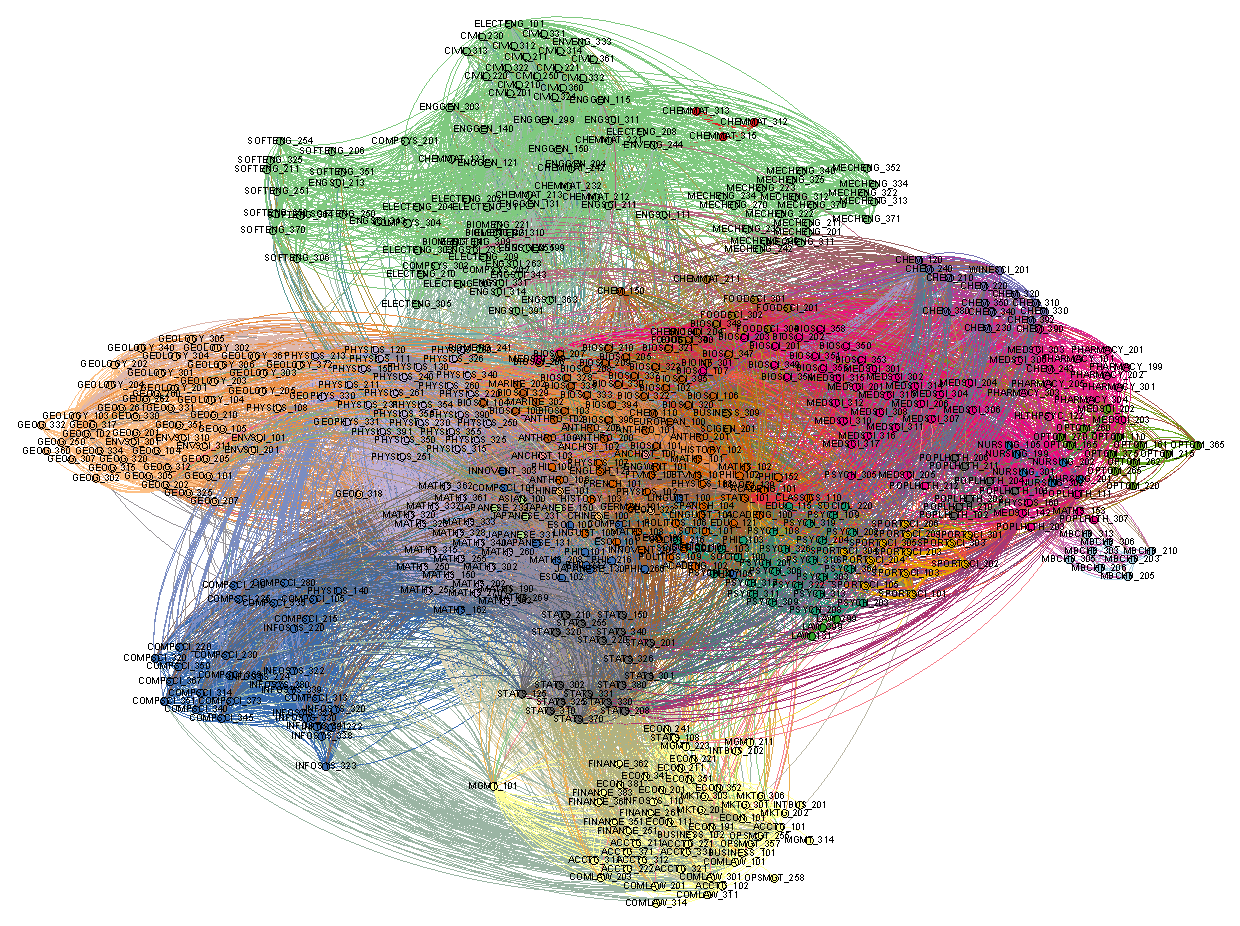
\includegraphics[width = \linewidth]{C3 - Bourdieu Networks/C3 - Fig2.pdf}\caption{\textbf{Student Course Network.\newline} 
A network representing the communities, or fields, of courses formed by students co-enrolling in course at the University of Auckland. Each node represents a course offered by the university, while links between nodes indicate instances where students took those two courses together within their undergraduate degree. Node colour indicates the community that a course belongs to. Communities were revealed in a two step process. Firstly, edges were filtered so only those with an RCP value over 1 were included. Secondly, the Map Equation software package\cite{Edler_2017} was used to partition the network into communities of courses, which can be interpreted as the underlying academic fields. The revealed fields are labeled in Fig \ref{Fig3}, and represent the various academic fields that students in our sample were enrolled in.}
\label{Fig2}
\end{figure*}


\begin{table}[!ht]
%\begin{adjustwidth}{-2.25in}{0in}
\caption{\label{Table1} \textbf{Compositions of the Communities Detected in the Co-Enrollment Network.}}
\begin{tabular}{|c|c|c|c|}
\hline
\textbf{Community} & \textbf{Count students\textsuperscript{a}} & \textbf{Proportion female\textsuperscript{b}} & \textbf{Total enrollments\textsuperscript{a}} \\ \hline
Ancient History & 150 & 0.48 & 205 \\
Biological Science & 5630 & 0.52 & 18600 \\
Chemical Materials & 20 & 0.35 & 60 \\
Chemistry & 1660 & 0.49 & 4180 \\
Chinese & 60 & 0.27 & 85 \\
Computer Science & 4405 & 0.28 & 22195 \\
Engineering & 980 & 0.36 & 9315 \\
Finance-Marketing & 1430 & 0.29 & 6735 \\
Food Science & 640 & 0.53 & 1505 \\
Geography-Geology & 1470 & 0.38 & 6095 \\
Japanese & 85 & 0.38 & 180 \\
Law & 170 & 0.46 & 240 \\
Liberal Arts & 6410 & 0.38 & 12750 \\
Medical Science & 4715 & 0.53 & 26790 \\
Nursing & 70 & 0.81 & 300 \\
Optometry & 550 & 0.61 & 1310 \\
Pharmacy & 645 & 0.58 & 2100 \\
Physics-Maths & 3060 & 0.25 & 12125 \\
Population Health & 200 & 0.57 & 510 \\
Psychology & 1440 & 0.52 & 4410 \\
Sports Science & 245 & 0.47 & 575 \\
Statistics & 1470 & 0.36 & 3985 \\
Surgery & 350 & 0.43 & 2800 \\ \hline
\end{tabular}
\begin{flushleft}\textsuperscript{a}Counts have been rounded to the nearest 5 to preserve confidentiality.
\newline
\textsuperscript{b}Proportions were formulated using original, unrounded values.
\end{flushleft}
\label{table1}
%\end{adjustwidth}
\end{table}


\subsubsection{Transverse Movements}
To investigate whether there are gender differences in UoA physics students moving from one academic field to another during their undergraduate degree (transverse movements), we build on the network outlined in the previous section. We take the same set of nodes, with the same community structures, but weight edges by the number of students who took course $i$ \textbf{before} course $j$. From this new directed network, we are able to assess the movements that students make between communities. To answer our questions regarding the transverse movements that students make from one field to another, we aggregate the number of movements from courses within community $m$ to courses within community $n$ (see Fig~\ref{Fig3}). For example, the courses in the \textit{Physics-Maths} community in Fig~\ref{Fig2} become a single Physics-Maths node in Fig~\ref{Fig3}. Outgoing edges between communities are aggregated into a single outgoing edge, with a weighting equivalent to the sum of all outgoing edges weights from nodes in the community. Edges between courses within a community are similarly aggregated, and are represented as self-loops (a link from a node to itself) in Fig~\ref{Fig3}. To investigate how transverse movements differ by gender, we calculate the Odds Ratio (OR) with 99\% Confidence Intervals (CI) of a female student moving from community $m$ to community $n$ over a male student. OR are generated using the following formula\cite{field2012discovering}: 

    $$\frac{A/C}{B/D}$$

where A is the number of female students who did move from community $m$ to community $n$, B is the number of male students who moved, C is the number of female students who did not move, and D is the number of male students who did not move. The null hypothesis in this case is that female and male students were equally likely to make a movement from one field to another. We visualize these results in two different ways: Fig~\ref{Fig3} shows the co-enrollment network with nodes representing communities and edges representing likelihoods, while Fig~\ref{Fig4} is a heat map in showing the gender differences in transverse movements. In Fig~\ref{Fig3} orange edges indicate a higher likelihood of female students going from community $m$ to community $n$, and purple edges indicate a higher likelihood of male students going from community $m$ to community $n$ (the direction of the movement follows a clockwise direction).  In Fig~\ref{Fig4} communities are indivated on the horizontal and vertical axes, with movements from community $m$ (horizontal axis) to community $n$ (vertical axis). Once again, orange indicates that a female student was more likely to make a move from community $m$ to community $n$, with color intensity representing a higher likelihood. 

\begin{figure*}[!ht]
\centering
 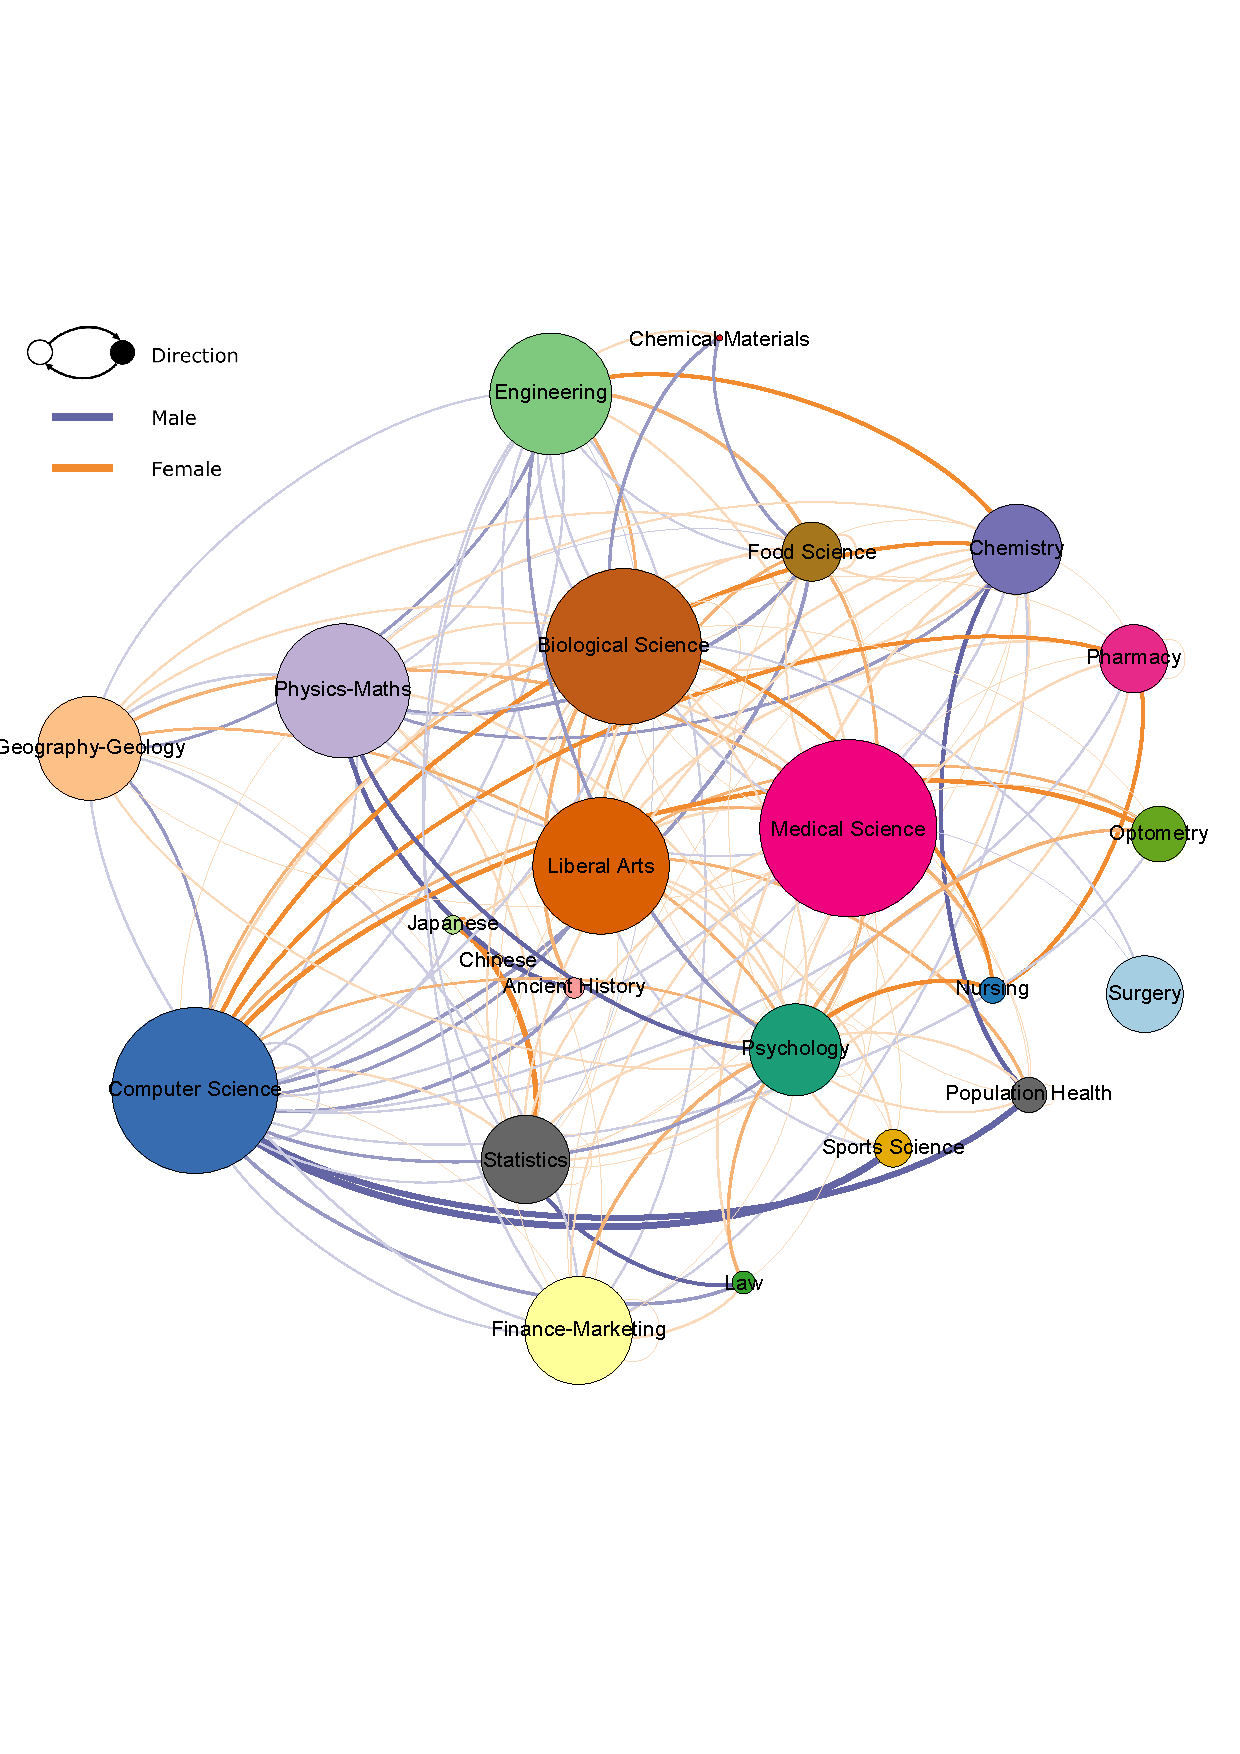
\includegraphics[width = \linewidth]{C3 - Bourdieu Networks/C3 - Fig3.pdf}
\caption{\textbf{Course Community Network.\newline} 
The above directed network represents the network seen in Fig~\ref{Fig2}, only the links within communities (i.e. links between courses belonging to the same community) and between communities have been split by gender and aggregated. Odds ratios comparing the likelihood of a female student taking a course in community $m$ and community $n$ were formulated, with the resulting values used as edge weights. The communities were labelled based on the range of courses that it is comprised of. Edges where female students were more likely to take a course in community $m$ and community $n$ are coloured orange, while edges where male students were more likely to take a course in community $m$ and community $n$ are coloured purple. When considering the flow between a pair of nodes connected by two edges, the direction of flow is outward following the link in a clockwise direction. The network shows that transverse movements from fields such as computer science and physics-maths to other domains tend to be female dominated, whilst movements into these fields are more male dominated.}
\label{Fig3}
\end{figure*}


\begin{figure*}[!ht]
\centering
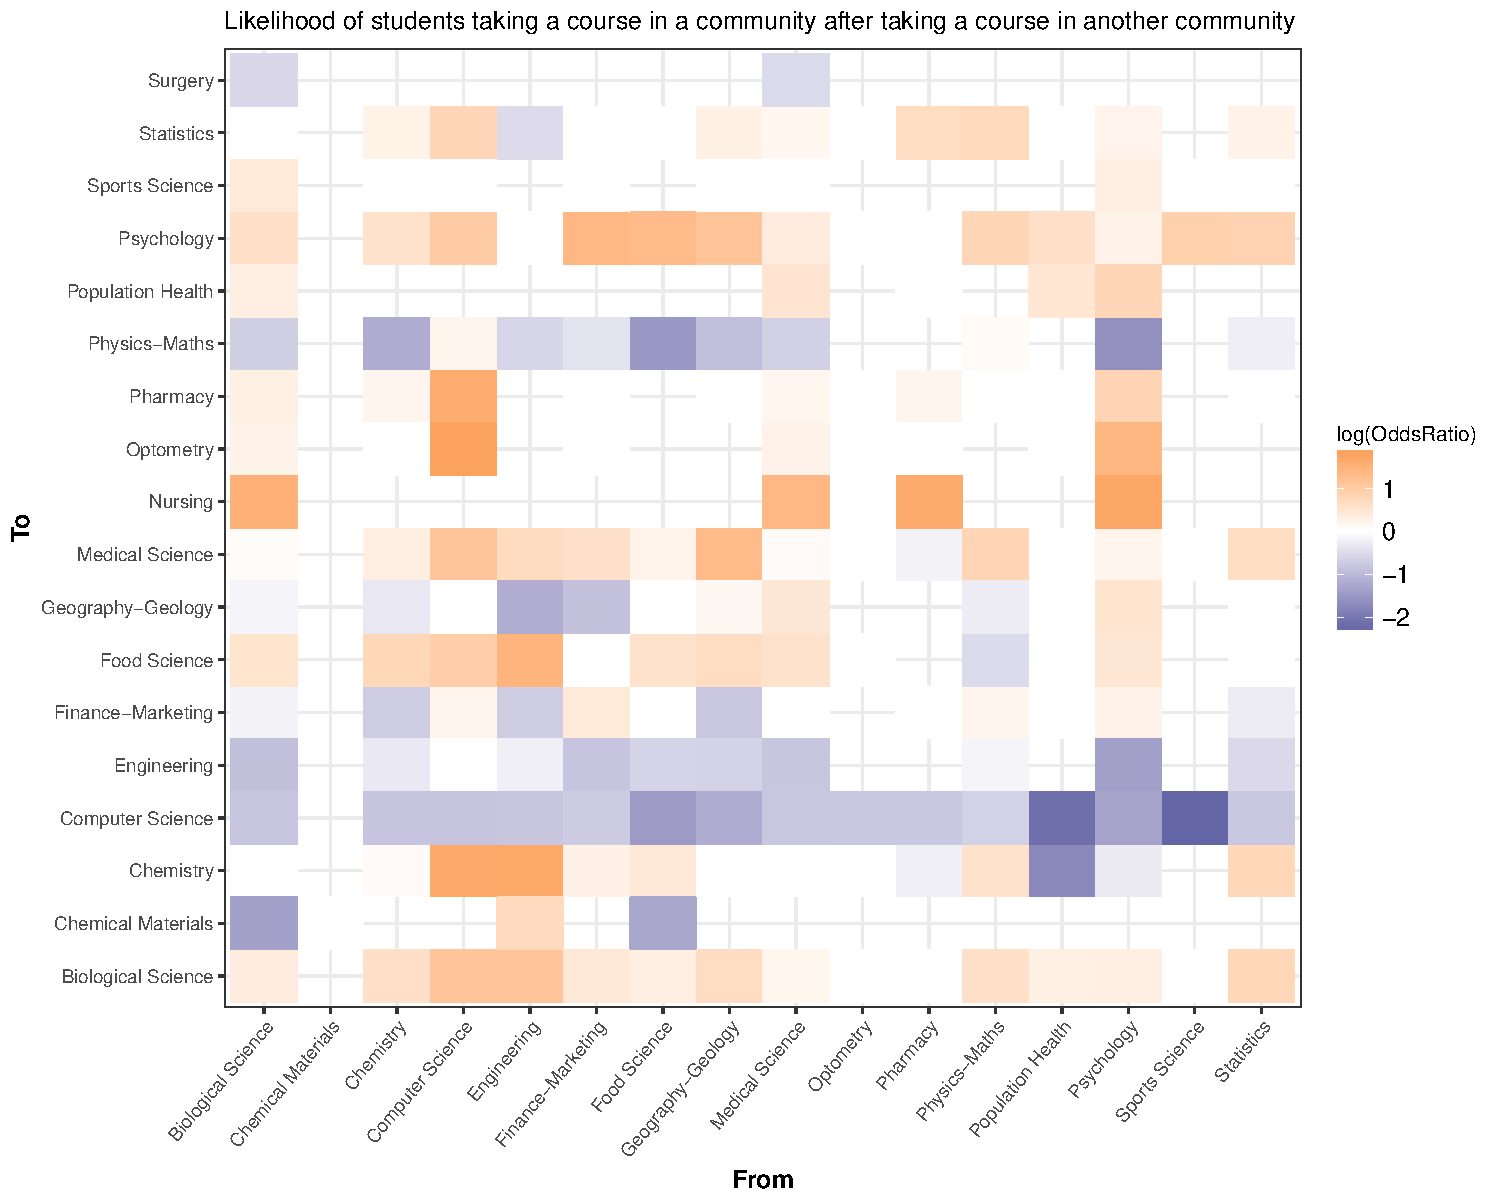
\includegraphics[width = \linewidth]{C3 - Bourdieu Networks/C3 - Fig4.pdf}
\caption{\textbf{Student Course Heat Map.\newline} 
The above heat map represents the same underlying data as that which is used in Fig \ref{Fig3}. The heat map makes clear the gender differences in the likelihood of students moving from one community to another. Orange areas represent instances where female students were more likely to take a course in community $n$ after taking a course in community $m$. Purple areas indicate male students were more likely to take a course in community $n$ after taking a course in community $m$. Areas that are white or empty indicate no significant relationship. Male students were consistently more likely to take courses in Computer Science and Physics-Maths after taking courses in each other community. Female students tended to be more likely to take courses in life science subjects (e.g., Biological Science and Psychology). }
\label{Fig4}
\end{figure*}

\subsubsection{Vertical Movements}
We also seek to investigate how male and female students with differing levels of prior achievement choose to invest their capital. Are there gender differences in the vertical movements (moving upwards or downwards in the objective rankings in a field) that students make from one stage to the next? Do male and female students with different levels of prior achievement choose to invest their capital differently? To understand the nature of students' vertical movements between within and between fields, we incorporate student achievement data into our previously established network. For each course, we have the student grade point unit score (i.e., their level of achievement). Our data set also includes an average high school achievement measure Grade Point Equivalent (GPE), for the majority of students in our network. This allows us to look at the transitions that male and female students make from high school to university study. 

We are particularly interested in the movements that students make going from high school to three specific stage one courses: AP1, AP2, and PLS. We also investigate the gender differences in vertical movements that students make from these physics courses to our detected fields, and between our detected fields. For our detected fields we calculate a Grade Point Average (GPA) score for each student (scored on a continuous scale of 0-9), in which we take the mean of the student's grade point unit scores for each course they took within the community. For example, the Physics-Maths GPA score will be a student's mean average grade point unit score for all of the courses they took within the Physics-Maths community.

As outlined by Bourdieu, an individual's power in a field is determined by the composition and volume of capital they hold \textit{relative} to other individuals. As our goal is to compare the relative vertical position of students within and between fields, we convert the achievement scores (GPE for high school, GPU for the key stage one courses, and GPA for the communities) into percentile ranks. Standardizing achievement in this manner facilitates comparisons across fields. Top achievers in a field will have a percentile rank score of 100, whilst low achievers will have a percentile rank score closer to 0. We can then compare the change in percentile rank scores for male and female students across our network. To describe the gender differences in vertical movements, we use independent 2-group Mann-Whitney U Tests (a non-parametric t-test) to test the median difference in percentile rank change between male and female students. Non-parametric tests were chosen as they are robust to outliers and skewed distributions\cite{erceg2008modern}, and we do not assume the distribution of rank changes to be normal. We were then able to determine whether there were any significant differences between male and female students gaining in relative performance across fields, with the null hypothesis being that there are no gender differences in percentile rank change. We report effect sizes in terms of the Common Language (CL) effect size\cite{mcgraw1992common}, which is robust, widely used and easy to interpret.\cite{erceg2008modern, lakens2013calculating, kerby2014simple} As described by Lakens\cite{lakens2013calculating}, the CL effect size indicates: ``the probability that a randomly sampled person from one group will have a higher observed measurement than a randomly sampled person from the other group.'' In our case, the CL effect size indicates the probability that a female student will have a higher change in rank after moving to a new field over a male student who made the same move. We also report the OR (with 99\% CI) of top, middle, and low achieving female students enrolling in different fields compared to their male counterparts. These achievement groups are based on percentile ranks of all students split into three equally sized bins. We explore the movements from high school to key stage one university courses specifically, and from key stage one physics courses to detected fields. 

\section{Results and Discussion}
Networks showing the revealed communities of courses that students take can be seen in Fig~\ref{Fig2} and Fig~\ref{Fig3}. Fig~\ref{Fig2} shows the network of courses offered by the University of Auckland (UoA) between the years 2009 and 2014, with communities indicating courses that tended to be taken together within students' undergraduate degrees (represented by the different colours). The communities included (in ascending order of aggregated course enrollments): Medical Science, Computer Science, Biological Science, Liberal Arts, Physics-Maths, Engineering, Finance-Marketing, Geography-Geology, Psychology, Chemistry, Statistics, Surgery, Pharmacy, Food Science, Optometry, Sports Science, Population Health, Nursing, Law, Ancient History, Japanese, Chinese, and Chemical Materials.

The use of Revealed Comparative Preference (RCP) in conjunction with the community detection revealed underlying academic fields in which physics student participated, as indicated by the combinations of courses that students enrolled in. Physics courses (including AP1 and AP2, the first prerequisites for a physics major at the UoA) and mathematics courses were located the same field, which we label \textit{Physics-Maths}. PLS, a physics course required for students wanting to study medicine, was located in the field of \textit{Medical Sciences}. We report the counts of students per community, with the percentage of female students, in Table~\ref{Table1}. Liberal Arts, Biological Science, and Medical Science were the three largest communities based on number of unique students enrolled in each field. Medical Science, Computer Science, and Biological Science were the largest communities in terms of total enrollments (an individual student may be enrolled in more than one course per field). In terms of the proportion of female students per community, Physics-Maths (0.25), Computer Science (0.28), and Chinese (0.27) were the most male dominated. Nursing (0.81), Optometry (0.61), and Pharmacy (0.58) were the most female dominated. 

The network and RCP approach provides a non-biased method of classifying the fields in which students are participating in. The use of RCP shows that disciplinary labels (i.e., `Physics') are imperfect in classifying the patterns of courses that students enrol in. Although PLS is a physics course, it has a higher affinity with the life sciences, and our community detection approach reflects this by locating PLS within the field of Medical Science. For example, the percentage of female students enrolled in \textit{all} physics courses (including PLS) was 40\%. Our community detection shows that female students only made up around 25\% of the main Physics-Maths community. The difference between these percentages is substantial, and raises important implications for the way in which universities report the number of students studying in different disciplines.

\subsection{Transverse Movements}
We first wanted to understand whether there were gender differences in UoA physics students moving from one academic field to another. Our results regarding these transverse movements (more detail is given in the table in \nameref{S2_Table}) show that female students were around 1.8 (OR $=$ 1.82, CI: 1.63-2.02) times more likely to take a course in Biological Science after taking a course in Physics-Maths, and 1.4 (OR $=$ 1.44, CI: 1.40-1.47) times more likely to take a further course in Biological Science after taking a previous Biological Science course. On the other hand, male students were around 2 (OR $=$ 0.51, CI: 0.48-0.56) times more likely to take a course in Physics-Maths after taking a course in Biological Science. There were no significant gender differences in students taking a course in Physics-Maths after taking a previous course in that community. Male students were consistently more likely to take a course in Computer Science after taking a previous course in another community, for example going from Biological Science (OR = 0.44,CI: 0.42-0.46), Physics-Maths (OR $=$ 0.52 , CI: 0.50-0.54), and Computer Science (OR $=$ 0.44, CI: 0.43-0.45).
 
The above results show differences in the transverse movements that students make between fields. Female students were nearly twice as likely to switch into Biological Sciences after Physics-Maths, with male students nearly twice as likely to go the opposite direction. Thus, the results of the current study show that gender disparities are evident, not only in the fields in which students choose to study (see Table~\ref{Table1}), but also in the transverse movements made between fields. These findings are in line with previous research that shows that the life science disciplines (biology, medicine etc.) tend to be more popular for female students, while physics, maths, computer science and engineering tend to be more popular for male students.\cite{NSF, Cunningham_2015,Kost_Smith_2010,Heilbronner_2012, Stevanovic_2013, InstituteofPhysics_2012, Smith_2011, EducationCounts_2016a, Kennedy_2014, Semela_2010} Male students were consistently more likely to switch into computer science regardless of prior field. This highlights the field of computer science as a key area of future investigation, especially in the context of New Zealand STEM education.

Whilst the above findings indicate gender disparities in student enrollments, it is important to consider the achievement levels of students who enter in to different fields, and whether achievement impacts on the movements that students make. We wanted to know whether there were gender differences in the persistence of UoA students in physics, accounting for student achievement. The question we now ask is where did male and female students with differing levels of prior achievement choose to invest their capital? We look specifically at students coming from high school, to the key stage one physics courses (AP1, AP2, and PLS) and to the disciplinary fields revealed in our network. 

\subsection{Vertical Movements}
We investigated the impact of student achievement on student enrollment in two ways. We firstly report the number of top, middle, and low achievers who made movements from high school to the key stage one physics courses (AP1, AP2 and PLS), and to the fields revealed in our network. We then assessed the vertical movements that students made by analyzing gender differences in the change in objective rankings within and between fields. We begin by reporting the progression of students from high school to university physics. High school students were split into three equally sized bands based on achievement rankings. As highlighted in Fig 5, the top achieving group is gender balanced (50\% female students), while the middle achieving (40\% female students), and low achieving groups (33\% female students), have fewer female students. 

\begin{figure*}[!ht]
\centering
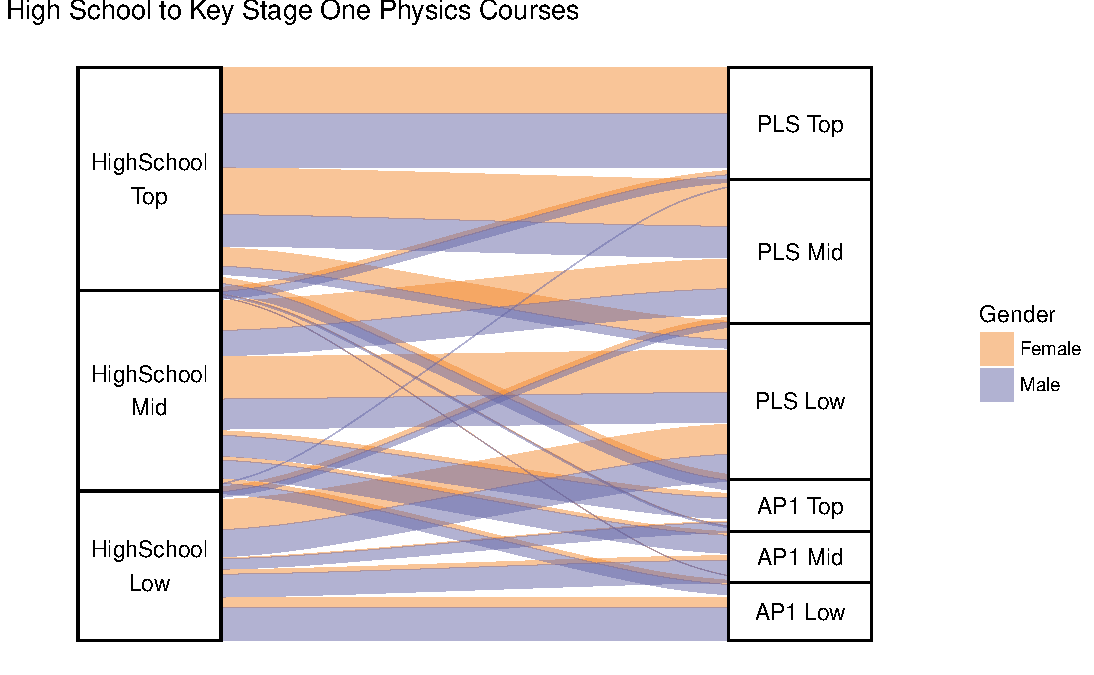
\includegraphics[width = \linewidth]{C3 - Bourdieu Networks/C3 - Fig5.pdf}
\caption{\textbf{Student Progression Alluvial.\newline}
An alluvial plot showing the progression of male (purple) and female (orange) students from high school to university physics split by achievement bands. Female students were equally represented among the top achieving high school group, but less well represented among the middle and low achieving groups. PLS (Physics for Life Sciences) and AP1 (Advancing Physics 1) represent the two main groups of physics students in our data. As shown in the alluvial plot, PLS was more popular than AP1, especially at the intersection of top achievers and female students.}
\label{Fig5} 
\end{figure*}

For students ranking in the bottom third of high school students (``low achievers''), 17.94\% of female students and 35.53\% of male students went on to study AP1. In comparing the odds of progression to AP1, we found that low achieving male students were 2.52 (OR $=$ 0.40, CI :0.30-0.52) times more likely to enter the main physics pathway at the UoA compared to their female counterparts. For students ranking in the middle third of high school students (``middle achievers''),  10.69\% of female students and 30.58\% of male students went on to study AP1. Middle achieving male students were 3.68 (OR $=$ 0.27, CI: 0.20-0.37) times more likely to enter physics at the UoA compared to their female counter parts. 

Our findings show that of the students who were ranking in the top third of students coming from high school (``top achievers''), very few chose to invest their capital in physics. Only 8.72\% of male students and 5.06\% of female students who were top achievers from high school chose to enrol in AP1. These percentages also indicate that from this top achieving group, male students were 1.79 times more likely to go to AP1 (OR $=$ 0.56, CI: 0.36-0.87). Thus, not only does it appear that physics is an unattractive option of top achieving high school students, but this is particularly true for top achieving female students. In contrast, 72.66\% of male students, and 88.35\% of female students from this top achieving group enrolled in PLS. Top achieving female students were around 2.8 (OR $=$ 2.84, CI: 2.10-3.83) times more likely than their male counter parts to follow this pathway. 

Our results provide a good indication that the life science fields tend to be viewed as high in symbolic capital (prestige), as they attracted a higher proportion of high achieving students. This echoes arguments that medicine is perceived as a high status career that is highly sought after.\cite{Wong2012} The fact that we did find differences in the choices to study PLS over AP1 suggests that physics is viewed as a less rewarding study path than the life sciences. Questions need to be asked about the way in which physics is presented to students in secondary school. Claussen and Osborne\cite{Claussen_2013} argue that science education needs to highlight the utility value of science in culture, scientific literacy, and employment. Students will choose to invest their capital in a field where they feel that they can get the largest return (be it in educational qualification, future employment opportunities, or enjoyment). Our findings suggest that within science education, physics needs to make a stronger case for its utility in order to attract high achieving students, in general, and female students in particular. This could be achieved by boosting science capital\cite{Archer2015a}, increasing the knowledge about the future value of physics courses in the employment market\cite{Archer2014}, and providing information on the utility of physics in everyday life. 

Increasing the value of physics and boosting the related capital of students within physics, although necessary, is likely an insufficient strategy to address gender disparities. In the context of previous research, it may be that our findings can be explained by the unwelcoming climate presented in the field of physics.\cite{Blickenstaff_2005, Kost_Smith_2010} Following Bourdieu's theoretical framework (Fig~\ref{Fig1}), we must also consider students' habitus. The affinities that students feel towards each scientific discipline is influenced from an early age by their experiences in, and perceptions of the field of science education. Using evidence from their life experiences, students enter into university with an idea of what discipline is `\textit{for me}'. For fields such as physics and computer science, where we found the most consistent gender disparities in enrollments, previous research suggests that students are influenced from an early age by the ``smog of bias''\cite{Kost_Smith_2010} that targets women. Through the combination of a myriad of factors, from the negative gender stereotypes\cite{Nosek_2009}, to the ways in which women's competence is unfairly questioned\cite{Moss_2012,Potvin_2016, ong2005body}, students will internalise (via habitus) the perception that physics is something men do, and where women are unwelcome.\cite{Archer_2013} Until the `smog of bias' is addressed, female students will continue to have constrained choice in science.

Whilst we could interpret the lower likelihood of a male student studying in the life sciences as resulting from possible obstacles also, we find this an unrealistic interpretation. The sizable representation of male students and researchers in the life sciences presently and historically, and the lack of negative factors that impact male students in this domain, mean that the life sciences are likely still a realistic study choice for male students. To put more simply, male students have more choice on where to invest their capital, whilst female students are more likely to face obstacles. The rules operating in the field of physics may require female students to make extra effort to appear competent and persevere in the field. As outlined by Ong\cite{ong2005body} in a study of minority female physics students: ``the ways in which women of color organize themselves to appear competent in the context of physics specify invisible rules about the strict boundaries around local scientific communities.'' The idea that women in physics may have to ``relegate social and cultural identities to the margins''\cite{ong2005body} in order to succeed in physics corresponds to Bourdieu's idea that individuals lacking in the `valued' cultural capital in a field may need to make sacrifices to get ahead.\cite{Bourdieu1984} 

Of the students from AP1 who ranked in the bottom third of achievers (low achievers), we found that 40.38\% of male students, and 28.29\% of female students progressed to AP2. Female students from this low achieving group were around 1.72 (OR $=$0.58, CI: 0.35-0.98) times less likely to progress from AP1 to AP2. There were no significant gender differences in the middle (OR $=$ 0.84, CI: 0.56-1.24) and top achieving (OR $=$ 0.77, CI: 0.49-1.21) AP1 students who went to AP2.

The above findings point to previous research that suggests that female students may be less confident in physics\cite{B_E_2013,Sharma_2011,Hofer_2016} and maths\cite{Else_Quest_2013, Sheldrake_2015}, or, rather, low achieving male students may be \textit{over-confident}. It may be that in our sample, gender differences in progression from AP1 to AP2 for middle and top achieving students were not present as the grades received offered evidence that they \textit{belong} in physics. For the low achieving students, belonging is not evidenced by their grades. Low achieving male students may be buffered by a habitus that, after years of socialization, predisposes them to physics. Female students, on the other hand, may be less likely to have this protective disposition. Whilst further research is needed to substantiate this claim, past research does suggest that students are more likely to make internal attributions of failure for female students in science (i.e., they fail because they are not good at it), and external attributions of failure for male students (i.e., unfavourable circumstances)\cite{LaCosse_2016}. Furthermore research by Ellis, Fosdick and Rasmussan\cite{Ellis_2016} found that female students are more likely to discontinue physics after taking an introductory calculus course, with female students also being more likely to cite lack of understanding as a reason for dropping out. This may also apply to students in our sample, as AP1 includes content that requires knowledge of calculus.

We also investigated the rank change for students moving from high school to the key stage one physics courses, and from those physics courses on to the fields detected in our network. We found no statistically or practically significant gender differences in the vertical movements in these pathways, with the exception of students going from high school to AP1. As indicated by Fig~\ref{Fig5} and \ref{Fig6}, we found that low and middle achieving female high school students were more likely to decrease their rank in the field (i.e., make a vertical movement downwards) in AP1 with this being significant. Comparing the ranking on a scale of 0-100 in high school and AP1, on average, low achieving high school female students went down around 6 ranks compared to their male counterparts (Difference in Position=$-5.71$, CI: $-8.57$ - $-2.86$), with the Common Language (CL) effect size being 0.40. This effect size means that if we were to pick a random male and female student and compare their change in rank, there would be a 40\% chance that the female student had a higher change in rank compared to the male student, or, conversely, there would be a 60\% chance that the male student had a higher change in rank compared to the female student. Middle achieving female students went down around 9 ranks relative to their male counterparts (Difference in Position=$-8.57$, CI: $-12.86$ - $-2.86$), with a CL effect size of 0.41. There was no significant gender difference in rank change for top achievers. 



\begin{figure*}[!ht]
\centering
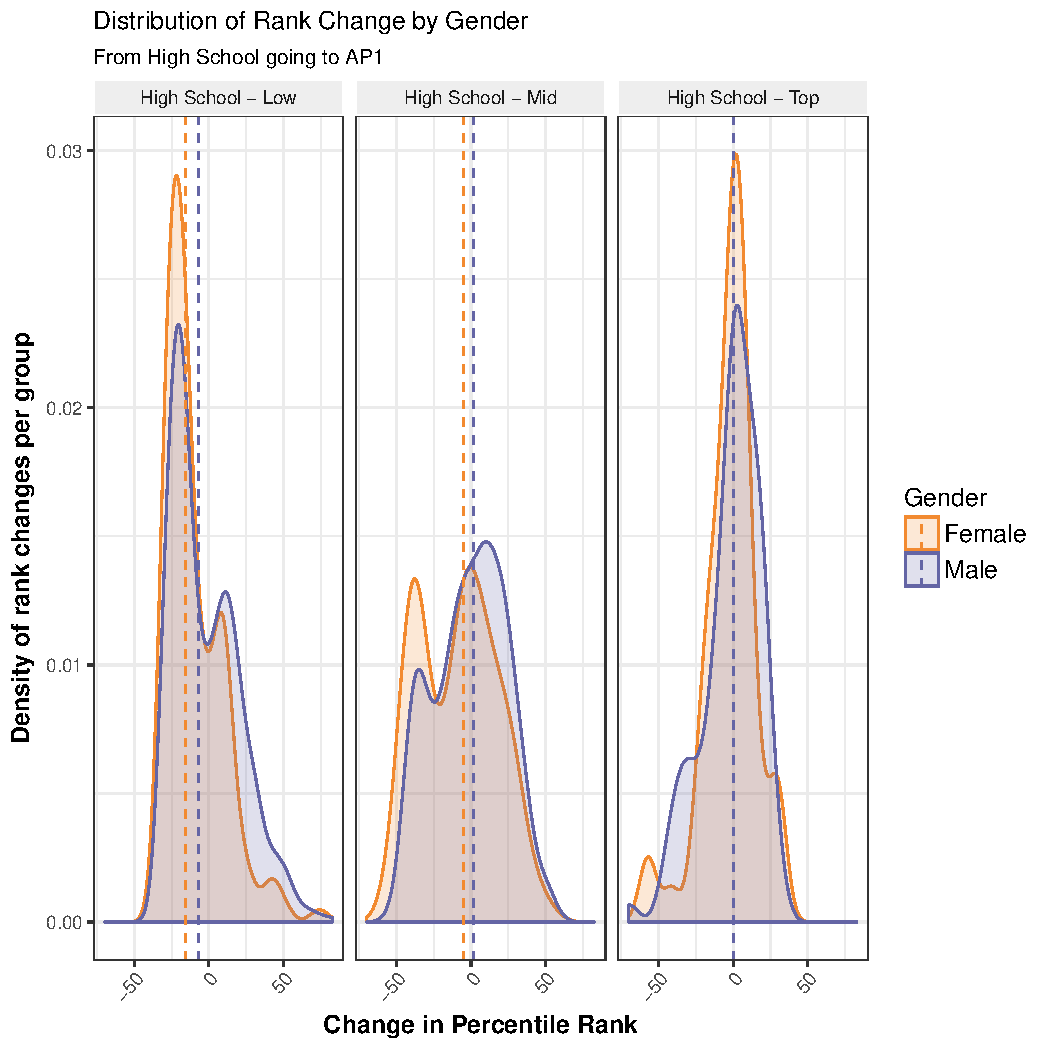
\includegraphics[width = \linewidth]{C3 - Bourdieu Networks/C3 - Fig6.pdf}
\caption{\textbf{Distribution of Rank Change by Gender and High School Achievement Group.\newline} 
The above density plots show the distribution of rank change going from high school to Advancing Physics 1 (AP1). Purple represents the distribution of rank changes for male students, while orange represents female students. The dotted vertical line show the median rank change per group. On average, low achieving female students went down 6 ranks compared to their male counterparts, while middle achieving female students went down 9 ranks relative to their male counterparts. There was no significant gender difference in rank change for top achievers.}
\label{Fig6}
\end{figure*}

These results somewhat echo the findings of Kost-Smith and colleagues.\cite{Kost_Smith_2010} They found that male students tended to outperform female students on post-test physics concept inventory scores, despite there being no gender differences in pre-test scores. Based on this, we would expect male students in our sample to also increase their relative position in the field of physics after first year study. With that being said, the gender differences in the vertical movements we did find for middle and low achieving students were relatively small, and non-existent for top achieving students. The top achieving female students in our sample who chose to progress in physics likely have a habitus that is just as congruent with physics as the male students (i.e., they feel that physics is `for them'). However, taken in the context with our other findings that female students were less likely to progress from high school to AP1, or from AP1 to AP2, questions must be asked about the distribution of physics-related capital and the development of physics habitus \textit{before} university education, particularly for middle and low achieving students. Many studies point to the late childhood and early teenage years as a key formative stages\cite{archer2013aspires,DeWitt2014,Baram_Tsabari_2010} for identity within science. Future studies of tertiary education in New Zealand should investigate the role of science identity in subject selection decisions further.

\subsection{Implications}
The current study offers a detailed account of the movements that students make through university physics. Our results show that female students were less likely to progress from high school to AP1, regardless of prior achievement, while low achieving female AP1 students were less likely to progress to AP2. The findings of the current study suggest that more needs to be done to ensure that physics is perceived as a viable option for female students and high achieving students (and particularly high achieving female students). This can be done by using interventions to boost the value that science capital holds in all areas of society. Echoing the arguments of Claussen and Osborne\cite{Claussen_2013} and Archer and colleagues\cite{Archer2012}, science education in New Zealand, and internationally, needs to highlight the utility value of physics in culture, in boosting scientific literacy, and employment. 

However, we argue that boosting the value and access to capital, despite being a necessary goal for boosting the numbers of students in physics, is insufficient to tackle gender disparities. Following our research framework, we should seek to transform the habitus of students to encourage them to invest their capital in physics. We need to continue to change the culture of physics so that it is more likely to be viewed as a viable study option. Whilst we do not want to force students to study in areas where they do not want to be, we echo the sentiments of Cheryan and colleagues\cite{cheryan2017some}, who state:
\begin{quote}
Just because women are excited to go into other fields does not mean that they would not have been equally excited to go into computer science, engineering, and physics if the cultures signaled to them that they belong there.
\end{quote} We need to transform the field of physics so that it signals to female students that they belong there. 

Previous research suggests that interventions to boost the number of female students graduating in physics would be most useful at stages of education prior to university\cite{cheryan2017some}, as intentions to study science can be formed by early secondary school.\cite{archer2013aspires,Baram_Tsabari_2010} Female students' self-concept in physics may be improved through exposure to supportive family members\cite{kelly2016social} and high school teachers.\cite{Hazari2017, kelly2016social}

The results of the current study do also indicate that more needs to be done to support the female students who have already chosen to study physics at university. This may take the form of increased academic support for low achieving students in particular. Universities can seek to provide group learning experiences in introductory physics\cite{Sawtelle_2012}, and more welcoming environments for female students in physics and computer science.\cite{master2016computing}

As outlined by Bourdieu, individuals fight to define the criteria of what is of value in the field. Individuals who hold power in the field have the means to change the culture of physics. As stated by Hilgers and Mangez\cite{hilgers2014introduction}:
\begin{quote}
    The chances that established actors will succeed in preserving the order [of the field] are, however, greater than the probability of subversion. The more legitimate an agent, the more her peers consume her products, and the more they consume her products, the more legitimate she becomes.
\end{quote}
Following this logic, culture change in the field may require forced institutional changes. Initiatives to help address the inequities faced by women already in the field\cite{Ivie_2013}, and to increase the representation of women in research and higher education\cite{AthenaSwan,Horizon2020} are important steps to fostering changes in culture. Through these initiatives, we signal to future students from all backgrounds that physics is somewhere where women belong. 

Beyond our research findings, the current study demonstrates the utility of using network analysis and Bourdieu together. Whilst network analysis serves as a good method for representing Bourdieu's concept of field, Bourdieu's theory provides a rich interpretive lens. Our approach carries many benefits over other, more simplistic frameworks, such as the leaky pipeline. Employing the concepts of field, capital and habitus allow us to understand the objective structure of physics, whilst respecting the subjective contexts in which students are placed. Doing so removes stigma that can be attached to students who `leak' from the physics education pipeline. Emphasizing the contexts that students are situated in allows us as researchers to place our findings in a broader context and formulate suitable interventions to boost the physics enrollments of underrepresented groups. 

\subsection{Limitations}
There are limitations to the current work that future studies should address. Firstly, our data set is limited to UoA physics students, and included only course selection and performance information, and minimal demographic information. We did not have data regarding the course selection information of students prior to university, whilst our measure of high school achievement was a general measure and not subject specific. More detailed data would have provided more information regarding students' educational trajectories. With that being said, our results show the utility of working with student record data. Our network analysis, whilst simple, also provides a strong framework for working with more complex data; for example, investigating the distribution of economic, cultural, social capital across the network.

Whilst we argue that our network analysis approach enables us to draw many conclusions from our data, our study would also have benefited from combining our quantitative analysis with qualitative measures. We have used a quantitative approach to defining the field, and used evidence from other research studies to draw conclusions from our data. Whilst this approach is informative, qualitative approaches can provide even more context specific details. Bourdieu highlighted the need to break the dichotomy between the aim of understanding the `objective reality' (the overall distributions of groups and relationships between them) and the aim of understanding ``not `reality', but agents' representations of it''.\cite{Bourdieu_1986} Surveys and interviews of students would provide contextual and fine-grained detail that would complement our quantitative network analysis. Qualitative analysis may also be a more appropriate way to investigate gender as a non-binary construct.  

Despite having access to information regarding the ethnicity of students, we decided not to present this information in the current analysis. This is due to the fact that preliminary analysis showed low cell sizes for ethnic groups other than New Zealand European and Asian students in physics, in particular M\={a}ori and Pacific Island students (these findings are available on request). When possible, future studies should make use of an intersectional research design (one that explores the interaction between gender, ethnicity, social class etc.). This is especially important when using a Bourdieusian framework to interpret results. As suggested by Bourdieu: ``The individuals grouped in a class that is constructed in a particular respect... always bring with them secondary properties''.\cite{Bourdieu1984} Understanding the intersection of student characteristics would allow us to include the secondary properties that Bourdieu speaks of. The authors are currently conducting further analysis to understand why there were low cell sizes for minority groups using data from earlier educational stages (i.e., secondary school). 

\section{Conclusion}
The current study investigated gender differences for undergraduate physics students at the University of Auckland (UoA) through the use of network analysis on student data, with an interpretive lens based on the work of Pierre Bourdieu. Our network analysis revealed the different academic fields in which students are situated. We outline the utility of networks in visualizing Bourdieu's concepts of vertical and transverse movements within and across fields. Analysis showed gender differences in transverse movements (moving from one field to another) consistent with gender stereotypes: female students were more likely to enrol in life science fields (Biological Science, Medical Science), while male students were more likely to enrol in the Physics-Maths and Computer Science fields.Analysis of a UoA student-course network revealed that female high school students are more likely to study life sciences at university compared to physics, and this is particularly true for high achieving students in this group. Furthermore, of the female students who did enter physics in their first year, low achieving students in this group were less likely to progress to further physics compared to their male counterparts. We relate these findings to Bourdieu's concepts of field, capital and habitus (Fig~\ref{Fig1}). High achieving secondary school students (especially female students) may see more of a return for their capital in the life sciences compared to physics. Whilst it may be that physics does a poor job of highlighting its value, we argue that female students will continue to suffer constraints in their subject selection until the `smog of bias'\cite{Kost_Smith_2010} in physics is addressed. As outlined by Kost-Smith and colleagues\cite{Kost_Smith_2010}, it is unlikely that a single factor can account for the gender disparities seen in physics enrollment. We suggest that the various factors that have been linked to the attrition of women from physics (e.g., negative gender stereotypes, lack of female role models etc.) culminates into a gendered habitus that increases the likelihood of students viewing physics as a field that men do and where women are unwelcome. We close by discussing potential avenues for addressing gender disparities, which focus on not only boosting access to, and the value of, physics related capital, but also transforming the culture of the field so that all students (and especially women) view physics as a feasible study option.





 
\chapter[The Impact of Science Capital on Self-Concept in Science][]{The Impact of Science Capital on Self-Concept in Science: A Study of University Students in New Zealand}

\section{Preamble}
The following work was published in Frontiers in Education on the... Coauthors included Kane Meissel$^1$, Kirsten Locke$^{2,3}$ and Dion R.J. O'Neale$^{2,3}$. The goal of the current article was to build upon the previous chapter which introduced Bourdieu's sociological theory and how it can be applied to science education. Following feedback from colleagues in the STEM Transformation Institute at Florida International University, I began to question how much information can be gained through administrative data. Administrative data can be explored to understand overall patterns in participation, but how much can it really tell us about the forms of science capital available to students, and how this relates to their internal dispositions? To go deeper, the decision was made to administer a survey, tailored to my research questions, to science students at the university of Auckland.

\footnote{$^{1}$School of Learning, Development, and Professional Practice, Faculty of Education and Social Work, University of Auckland, Auckland, New Zealand \\
$^{2}$School of Critical Studies in Education, Faculty of Education and Social Work, The University of Auckland, Auckland, New Zealand \\
$^{2}$Te P\={u}naha Matatini, University of Auckland, Auckland, New Zealand }



\begin{abstract}
Understanding factors that contribute to students' self-concept in science is an important task in boosting the number of students studying science and retaining students in science fields. A questionnaire was administered to science students at the University of Auckland in New Zealand (N = 693) to test a theoretical model of science self-concept tied to the work of Pierre Bourdieu. In this model, a student's social capital (i.e., relationships with parents, teachers and peers) and cultural capital (i.e., science related resources) are seen as key determinants of a student's belief that science is a domain in which they can succeed. Results from a Structural Equation Model (SEM) show that, of the factors included in the model, exposure to passionate science teachers during high school was the main predictor of science self-concept for our sample of university science students, while having peers who value science was also found to be important. Interestingly, science-related resources and parents’ value of science were not significant predictors of science self-concept, but the number of university generations in the family did have a positive association.  Students who self-identified as male had higher levels of science self-concept, even after accounting for social and cultural factors in our theoretical model.  Implications of these findings are discussed in the context of the field of science education and Bourdieu's sociological theory.
\end{abstract}


\section{Introduction}
\label{intro}
Much research has been dedicated to understanding who chooses to study science at university, and what factors influence retention and completion of university science degrees. One particular factor that is associated with retention is students' science self-concept. Broadly speaking, self-concept is an individual's perception of their self \citep{shavelson1976self}, while science self-concept relates to a individual's belief regarding their general competency in science \citep{jansen2015students}. Understanding students' science self-concept is important for several reasons. Students who feel that they are good at science are more likely to have better outcomes in science classes \citep{uccar2017role,tighezza2014modeling,chang2008science,peters2013examining}, hold aspirations for further study \citep{mujtaba2018students}, and graduate from university \citep{larson2015predicting}. In turn, graduating from university tends to lead to better life outcomes in general \citep{Oreopoulos_2007}, and greater economic outcomes \citep{norton2016mapping,mahoney2013moving}. Research on factors affecting student's self-concept in science also has important implications for governments, as they seek skilled workers in Science, Technology, Engineering and Mathematics (STEM) to help gain economic prosperity and growth \citep{pricewaterhousecoopers2015smart}. In New Zealand, the education system is not only charged with producing an increase in the number of skilled workers in STEM domains, but also with producing confident learners. This message is made clear in the official high school curriculum \citep{NZC}:

\begin{quote}
   The New Zealand Curriculum is a clear statement of what we deem important in education. It takes as its starting point a vision of our young people as lifelong learners who are confident and creative, connected, and actively involved.
\end{quote} 

A wealth of research has shown that disparities in tertiary science participation exist across the intersection of gender, ethnicity and social class \citep{reynolds2011change,meehan2017explaining}. Students from high Socio-Economic Status (SES) backgrounds are more likely to realise tertiary education goals \citep{reynolds2011change}, whilst interest in science also tends to differ across SES, gender \citep{cheryan2017some}, and ethnicity \citep{Wong2016ScienceStudents}. Previous theorists have used metaphors, such as the \textit{gender filter} \citep{Blickenstaff_2005} and the \textit{smog of bias} \citep{Kost_Smith_2010} that consider the way contextual factors impact on student outcomes. For example, \cite{Kost_Smith_2010} argue that gender disparities can not be attributed to one specific factor, but instead there are a range of factors and small effect sizes that combine to produce inequity. Differing levels of self-concept may be one such factor that contributes to the disparities observed in STEM participation. For example research shows that female students tend to report lower levels of self-concept in mathematics and science \citep{Else-Quest2013}, and gender differences in confidence may persist even when accounting for actual achievement \citep{Ellis_2016}.

A student's self-concept does not exist in a vacuum. It is important to consider the factors that relate to students' self-evaluations of their ability in STEM domains. Why do gender, ethnicity, and social class often share a relationship with students' beliefs regarding their competency in science? The goal of this article is to explore the factors affecting science self-concept further, using a theoretical framework that can answer this question. More specifically, we hope to highlight the way in which students' self-concept in science is rooted in societal structures. To do this, we employ the sociological theory of Pierre Bourdieu \citep{Bourdieu1984}. Recent research has made use of Bourdieu's sociological theory as a framework for understanding the uneven patterns in student interests and pursuits in science \citep{archer2013aspires,Archer_2015,turnbull2019bourdieu}. Bourdieu's theory enables us as researchers to place individuals in the context of their environment, and to understand how social, cultural, and historical factors structure the world in which individuals live, and the internal dispositions they hold. The following section outlines Bourdieu's theory in more detail, with specific reference to \textit{science capital} \citep{Archer_2015}.

\section{Bourdieu and Science Capital}
\label{sciencecapital}
While applications of Bourdieu's sociological theory are wide ranging, it has been increasingly used as a theoretical framework to understand student's experience in science education \citep{Archer2015a}. Bourdieu's sociological framework encourages us to explore how resources are distributed across society, and how external structures in society relate to an individual's internal dispositions.  According to \citet{Bourdieu_1986}, resources, or \textit{capital}, can take various forms; such as economic, cultural, and social. Economic capital refers to an individual's financial resources (e.g. money, investments). Cultural capital refers to an individual's non-financial resources, such as the objects they own (e.g. books, clothing, furniture), or the characteristics they embody (e.g. accent, posture). \citet{Bourdieu_1986} defines social capital as that aspect of our relationships with other individuals that enables us to generate economic and cultural capital. With all forms of capital, the value is determined by the \textit{field} in which it is being used. To give a basic example, owning science books may be of value for someone studying in the field of science, but this is of less value to someone studying opera. Contemporary research has applied Bourdieu's sociology to explore student outcomes in the field of science specifically by using the concept of \textit{science capital} \citep{Archer2015a}. Science capital has been described by \cite{Archer2014} as a:
\begin{quote}
conceptual device for collating various types of economic, social and cultural capital that specifically relate to science --- notably those which have the potential to generate, use, or exchange value for individuals or groups to support and enhance their attainment, engagement and/or participation in science.
\end{quote}
Science capital provides a framework that is relatively simple to interpret and can facilitate our understanding of students' access to resources and the value that they derive from them in science. The following section describes the economic, cultural, and social forms of capital that are important to consider when exploring student's self-concept in science.  We begin by describing the importance of financial assets (economic capital) and non-financial assets (cultural capital) in education. We then describe the importance of shared relationships with others (social capital) which can provide access to resources. We summarise these social relationships in terms of teachers, peers, and family. We finish this section with a discussion of how these resources relate to the way in which students may view themselves in the field of science through Bourdieu's concept of \textit{habitus} and the psychological construct of self-concept. 

\subsection{Economic and Cultural Capital}
Simply put, the concept of economic capital refers to an individuals' financial assets (e.g., money). The benefits of economic capital are well studied and relatively easy to interpret. Previous research has shown that family income and wealth are large predictors of educational success \citep{shapiro2013roots, blanden2004family}. In New Zealand, a 30 year longitudinal study conducted by \citet{gibb2012childhood} found that childhood family income is a strong predictor of educational achievement in later life. As outlined by \cite{Bourdieu_1986}, the value of economic capital comes from its exchange value. For example, students from economically wealthy families are likely able to afford books, laptops, and other aids to study. In paying for these objects, students are exchanging economic capital for non-financial assets. Bourdieu categorizes these non-financial assets under the term cultural capital, and it is through cultural capital that educational advantages are accumulated. Recognising the role of non-financial forms of capital, and with it the social relationships that facilitate access to capital, is complex. In doing so, however, we are able to develop a theoretical model of social class that takes into account factors beyond economic wealth. 

Cultural capital refers to the non-financial resources an individual has at their disposal \citep{Bourdieu_1986}. Cultural capital is a complex concept as it is manifested in the objects that one owns (e.g., books, furniture, clothing), or embodied (e.g., in our posture, accent, bodily physique). In the context of science, cultural capital may take the form of objects that are used, such as chemistry sets, laptops, or books. Students may also boost their cultural capital in science with access to other science-related resources, such as visiting science museums \citep{Dawson2014} or after-school science clubs \citep{mujtaba2018students}. Cultural capital can play an important role in students' progression to university study \citep{aschaffenburg1997cultural}. This is echoed in the field of science education, where research has found that access to science related cultural capital is associated with decisions to study science further in high school \citep{mujtaba2018students}, and at university \citep{Lyons_2006}.

The manner in which students embody their cultural capital may also carry different value in science. Scientists are typically viewed as old, white males \citep{Nosek_2009,Barthelemy_2016} and individuals who differ from this stereotype may face barriers to acceptance in the field \citep{ong2005body}. Research has shown that women tend to be viewed as less competent in science solely in terms of their gender in many different roles, whether it involves a student's application to a lab assistant role \citep{Moss_2012}, or students' evaluation of their science teachers quality \citep{Potvin_2016}. 

\subsection{Social Capital}
While economic and cultural capital are important factors to consider in relation to self-concept, social capital is especially important. Social capital refers to value that is gained through relationships with others. This value can be viewed in terms of the economic and cultural capital that can be mobilised through relationships, but also through the impact of relationships on students internal dispositions \citep{Adler2017}. Having social relationships with individuals who hold valuable forms of capital is highly beneficial. For example, for a student studying at university, having parents who also studied at university may lead to better outcomes. These students are not only more likely to have access to educational resources (objectified cultural capital), but they may also be exposed from an early age to an academic way of life (embodied cultural capital). The following section details three valuable sources of social capital for students studying science: teachers, peers, and family.

\subsubsection{Teachers}
One of the most important forms of social capital for students is the student-teacher relationship. The value of this relationship is derived from several factors. Firstly, the content knowledge that teachers hold is an important form of cultural capital for students \citep{goldhaber2000does,wayne2003teacher,keller2017impact}, as it gives students access to knowledge. Students who have access to teachers with more content knowledge are more able to derive value from their relationship. However, it is also important to consider that content knowledge is transmitted as a function of the quality of the student-teacher relationship. The attitudes and behaviours of teachers can significantly impact on the interest students hold in STEM \citep{keller2017impact} and the way in which students see themselves in science. As outlined by theorists such as \cite{bandura1986explanatory} and \cite{siegle2007increasing}, teachers can boost their student's belief that science is somewhere that they belong by encouraging them and recognising their ability. For example, students who feel recognised as being good at physics are more likely to hold further interest in physics \citep{Hazari2017}. Through a Bourdieusian lens, recognition provides a signal to students that the field is somewhere they belong. Studies of classroom environments have continuously shown that positive teacher-student interactions are a strong source of interest in science \citep{osborne2003attitudes,keller2017impact}. \cite{mujtaba2018students} found that encouragement was an especially important influence in students aspirations to study chemistry. The social capital provided by teachers may be particularly important for students choosing to study in fields where they are members of an underrepresented group, or where their capital is undervalued by those with power in the field.


\subsubsection{Peers}
It is also important to consider the impact of students' social relationships with their peers in science outcomes \citep{osborne2003attitudes}. Adolescence is a time where individuals begin to be increasingly influenced by their peers \citep{douvan1966adolescent}, which can impact on academic engagement and achievement \citep{ryan2000peer} and students may be subjected to group norms that influence the decisions they make about future study \citep{brown1986perceptions}. Following this, it is no surprise that individuals belonging to friendship groups that value science are more likely to have motivations to pursue science further \citep{robnett2013friendship}. Other research shows that students' persistence in STEM domains at university may be influenced by their academic peer groups \citep{Ost_2010}.

\subsubsection{Family}
Finally, students' social capital is bolstered by their relationships within the family. Parents' educational expectations for their children is a key predictor of educational aspirations \citep{wu2015early}. In science, \cite{Lyons_2006} found that parents' attitudes towards educational qualifications and encouragement were important factors relating to students' decisions to study science. Students with highly educated parents are also much more likely to fulfil goals of attaining tertiary qualifications \citep{reynolds2011change}, while students with parents who are employed in STEM occupations are more likely to choose to major in STEM at university \citep{moakler2014college}. These findings point to Bourdieu's concept of social reproduction, where the social position of families are transferred across generations. Parents who are university educated may be more likely to engage in the concerted cultivation of children --- the process of deliberately building cultural capital that is valued by educational institutions \citep{lareau2011unequal}. Parents from higher SES backgrounds may hold higher educational expectations for their children \citep{carolan2015does}, whilst they may also be more involved in their children's education \citep{cheadle2011quantitative}.  Beyond the deliberate cultivation of their children, parents who studied science at university are also more able to use science-related discourse which is an important manifestation of cultural capital \citep{Lyons_2006,bernstein1971class}.\footnote{It is important to note that we do not suggest that the cultural capital espoused by those who are privileged is `better', only that it carries more value in the field of science education. Even though science is commonly perceived as having a `culture of no culture' \citep{traweek2009beamtimes}, the ways of teaching, assessing, and valuing student's capital is predominantly defined by those with power in the field of science --- historically western, male, and wealthy.}  The role of the family goes beyond typical forms of social capital, as the family provides the context in which individuals develop their identity. For this reason, family-related factors can be strongly tied to Bourdieu's concept of habitus.  

\subsection{Habitus}
As previously discussed, students' experiences within fields and their interactions with resources may begin to be embodied physically as embodied cultural capital. At the same time, students also embody these experiences \textit{mentally}. The mental embodiment of capital can be summarised by Bourdieu's concept  of \textit{habitus}. Bourdieu defines habitus as the internal dispositions that an individual holds that generate practices within the field. While an individual's volume of capital may determine their position in the field, their habitus determines their disposition towards the field \citep{bourdieu1992invitation}. Habitus represents an individuals' internalisation of society --- the resulting mental structure of the process commonly referred to as socialisation \citep{Nash1999}.

For Bourdieu, habitus is the mechanism which mediates between structure and agency. Students internalise the environment in which they are placed and make judgements on what is possible and realistic ``for them''. A student's family background is likely to have an integral role in shaping habitus. Students from families that are familiar with university or that have a history of working in science related fields may be more likely to have internalised dispositions that see science as something that is for them. A student's habitus is influenced by their familial context \citep{Dimaggio1982}, with some theorists pointing to the concept of ``family habitus'' as a tool to understand how family resources, values, and lifestyle choices are internalised by children \citep{Archer2012,tomanovic2004family}. The resources available to students through their family are thus extremely important, not only because they offer objectified forms of cultural capital, but also because they offer exposure to ways of thinking and understanding that have been historically proven to be valued by educational institutions. Students may be more likely to view science as a realistic study choice, and university as a possible destination, if they have parents who have modelled these trajectories previously \citep{Lyons_2006}. 

While family provides the context in which habitus is established, habitus is also informed by broader cultural groupings that individual identify with, and their experiences in other contexts, such as school. \citet[p.101]{Bourdieu1984} stated that if individuals are exposed to ``homogenous conditions of existence'' (i.e., similar life experiences) individuals will have similar habitus. In this sense, habitus can take on a collective quality where members of the same group are socialised in similar ways, predisposing them to hold similar dispositions. For example, \citet{Edgerton2014} use the concept of \textit{gendered habitus} to explain how gender socialisation relates to gender disparities in educational achievement. Research also suggests that  contexts outside of the family, such as school and peer groups, become increasingly important as students progress through education, while the impact of the family may diminish \citep{holm2011dealing}.   

Much research has discussed applications of habitus in education research \citep{Reay_2004,Nash1999}, although the concept is often criticised for being too complex \citep{goldhaber2000does} and difficult to operationalise \citep{dumais2002cultural}. Most research on habitus has been qualitative, but, as outlined by \cite{mu2014heritage}, there is an increasing need to consider quantitative applications of habitus. As habitus represents the internalisation of broader social structures, it takes on a collective quality that operates across social groups. While qualitative methods may be more able to describe individual experiences of habitus, quantitative methods are able to explore this collective quality of habitus. The current study  operationalises habitus quantitatively through the use of a science self-concept inventory. The construct of science self-concept was chosen as it is can be theoretically tied to arguments outlined by Bourdieu regarding habitus \citep{mu2014heritage,bodovski2014adolescents}. The following sections will describe self-concept in more detail and explain its relevance to Bourdieu's theory and the current study.   

\subsection{Self-concept}
\label{selfconcept}
While quantitative applications of habitus in education research are relatively rare, quantitative applications of self-concept have been more widely used, operationalised and validated \cite[e.g.][]{marsh2014academic,hattie2014self}.   Despite much variety in definitions of self-concept existing in research \citep{shavelson1976self}, self-concept can be broadly defined as the way in which an individual perceives their self \citep{rosenberg1979conceiving,shavelson1976self}.  As outlined by \citet[p.488]{shavelson1976self} ``Self-concept may be described as: organized, multifaceted, hierarchical, stable, developmental, evaluative, and differentiable.'' In basic terms, self-concept is an individual's judgement about their general competence in a domain \citep{jansen2015students}, which can be general (i.e. ``I am good at school'') and specific (i.e. ``I am good at science at school''). In many ways, self-concept is thus theoretically similar to habitus. Self-concept \citep[p.488]{shavelson1976self} and habitus \citep{Nash1999} are both multifaceted in that they operate across general and specific domains. They are also both relatively stable \citep[p.488]{shavelson1976self} and durable \citep{Bourdieu1984}, although both are subject to change when influenced by environmental sources located outside of the individual, such as the appraisals of others \citep{bong2003academic}. 

Although we identify similarities between self-concept and habitus, it is important to note that we do not consider them to be two different technical terms referring to the same underlying construct (a \textit{jangle fallacy}). While habitus is the internal, deeper ``system of dispositions'' \cite[p.471]{Bourdieu1984} that generates practice, often operating ``below the level of consciousness'' \cite[p.466]{Bourdieu1984}, self-concept is a perception one has of their self (i.e., ``I am good at science'') . While habitus includes domain-specific self-perceptions of competence, it also encompasses an ``estimation of chances'' \citep[p.76]{bourdieu1977outline} that guides future practices and dispositions (i.e., ``is science \textit{for me}?''). Self-concept may be viewed as an aspect of habitus that can be scrutinised through introspection. This point is argued by \citet[p.395]{bodovski2014adolescents}, who suggests that we may view both general and area-specific self-concepts as ``illustrations of different aspects of habitus.'' 

Despite the conceptual differences between habitus and self-concept, we argue that scores on inventories assessing self-concept can be productively interpreted through a Bourdieusian framework, and this has been evidenced in prior research \citep{dumais2002cultural}. As habitus may operate under the surface or unconsciously, it is a difficult concept to measure psychometrically, while self-concept is easier to assess. Importantly, the decision to interpret self-concept in terms of student habitus is necessary as it: ``ensures that the research focus is always broader than the specific focus under study'' \citep{Reay_2004}. In other words, using the concept of habitus facilitates the understanding of how an individual's self-concept is generated in relation to the socio-cultural context in which an individual lives. Given the similarities between self-concept and habitus, self-concept inventories are an appropriate and useful tool to explore an individual's habitus. 

Few New Zealand based studies have explored university students' self-concept or beliefs regarding their academic competency \citep{dalgety2006exploring,murphy2018determinants}. In one such study, \cite{dalgety2006exploring} explored the self-efficacy of first year university chemistry students in New Zealand across three time points in an academic year. They found male students tended to report higher scores in specific items related to self-efficacy (for example in their belief that they could achieve a passing grade in a chemical hazards course). While the work of \cite{dalgety2006exploring} offers many insights into student's internal dispositions at university in the context of New Zealand, the lack of research in this area, especially within the last decade, is a lacuna to be filled. 

\subsection{The Current Study}
\label{sec:3}

The current study seeks to address these two gaps in the research by exploring the relationship between science capital and self-concept in science for university students in New Zealand. More specifically, we apply Pierre Bourdieu's \citep{Bourdieu_1986,Bourdieu1984} concepts of capital and habitus to explore the interaction between students' access to resources and internal dispositions. Whilst the factors affecting outcomes in science are wide-ranging 
\citep{osborne2003attitudes}, we focus on the impact of science-related resources and social experiences in science on students' self-concept in science. In doing so, we are able to assess the impact of social class on self-concept, but using a definition of class defined in terms of \textit{capital} (social, cultural, and economic resources), as opposed to solely economic wealth. Our specific hypotheses are as follows. We expect:
\begin{itemize}
    \item Higher levels of science-related social and cultural capital to be associated with higher levels of self-concept in science. 
    \item Relationships with high school teachers will be the most important form of social capital. This is based on the idea that teachers are experts in the field and their judgements provide the most domain-specific feedback. In terms of habitus, students will be more likely to internalise the idea that they are good at science if they have an expert (the teacher) encourage them and/or recognise their ability. 
    \item Male students will have higher levels of self-concept than female students. This is based on previous research that points to gender disparities in confidence in science and mathematics \citep{Else-Quest2013,Ellis_2016}. 
    \item The number of university generations within a student's family, and having parents positively orientated towards science will be positively associated with self-concept. We would expect students who have available academic role models in their family to have a habitus that is predisposed to university science study. Such students will be more likely to  hold the belief that university is somewhere where they belong, and somewhere that they can be successful, because that is what their family does. 
\end{itemize}
While acknowledging that differences in science self-concept may exist across ethnic groups, the decision was made to exclude ethnicity from the current study. This decision was made to be consistent with kaupapa M\={a}ori values, a research position specific to the context of New Zealand that acknowledges the right of M\={a}ori (the indigenous population of New Zealand) to self-determination. This means that research concerning M\={a}ori should be done with M\={a}ori, and for the benefit of M\={a}ori \citep{walker2006exploration}. We seek to acknowledge our responsibility as researchers by elucidating the patterns found in the current study through a separate qualitative research project. This approach enables students from historically marginalised groups, such as M\={a}ori and Pasifika, the opportunity to have their own voices heard. This qualitative piece seeks to minimise the risk of deficit-theorising by allowing for more depth and nuanced understandings of M\={a}ori and Pasifika experiences in science. Future work should consider ways of knowing and constructing science and culture that are grounded in M\={a}ori ways of knowing, such as M\={a}tauranga \citep{hikuroa2017matauranga}. We hope that the results of the current study can aid in this endeavour.

\section{Methodology}
\label{method}
%\subsection{Data}
%\label{data}
During the first semester of 2019, an online questionnaire was administered to science students at the University of Auckalnd (UoA) via email following approval from the UoA Human Ethics Committee. In order to boost the rate of response, the questionnaire was designed to be quick (10 minutes), consisting of 48 items. Questionnaire responses were anonymous, with the exception of students who left their email to be entered into a prize draw. In total, 693 students consented to participation and completed the questionnaire, with a mean age of around 19 years old (the sample is summarised in Table \ref{tab:Sample}). 

\begin{table}[ht]
\centering

\begin{tabular}{lcccc}
\hline
& N   & Count & Percent    \\ \hline
Male                                                         & 685 & 247 & 0.36   \\
Female                                                       & 685 & 431 & 0.63   \\
Gender Diverse                                               & 685 & 7 & 0.01   \\
Euro                                                         & 693 & 367 & 0.53   \\
Asian                                                        & 693 & 305 & 0.44   \\
Pasifika                                                      & 693 & 28 & 0.04    \\
M\={a}ori                                                        & 693 & 48 & 0.07 \\
MELAA*                                                        & 693 & 21 & 0.03  \\
Other Ethnicity                                               & 693 & \textit{S} & 0   \\
& & &  \\ \hline
& N & Mean & SD \\\hline 
Age** & 594 & 19.93 & 3.65 \\
Parent Job  (0-4) &  681 & 2.61 & 0.71 \\
Uni generations (0-3)                                        & 687 & 1.67 & 1.04 \\ \hline
\end{tabular}
\caption{Sample description. Counts and percentages of categorical characteristics, and means and standard deviations of ordinal characteristics. Individuals self-reported gender which was then categorised into male, female and gender diverse groups for reporting purposes. Participants were given the option to  self-identify with multiple ethnic groups, which means that percentages do not total to 100.  *Middle Eastern, Latin American, or African. **Mature students (those with a recorded age over 24) were excluded from analysis (n $=$ 42). \textit{S} suppressed due to low cell size.} 
\label{tab:Sample}       % Give a unique label
\end{table}

The questionnaire asked students for factual information about themselves, and also questions regarding five latent constructs informed by and adapted from the work of \cite{dewitt2011high}. The constructs, outlined in our conceptual model (see Figure \ref{fig:ConceptualModel_C4}), included self-concept in science (Science Self-Concept; 5 items), experience of high school science teacher quality (Science Teachers; 5 items), parental attitudes towards science (Science Parents; 4 items), peer attitudes towards science (Science Peers; 4 items), and access to science-related resources (Science Resources; 5 items). The first four constructs were measured through items asking students to rate their agreement regarding a statement on a Visual Analog Scale (VAS), with scores ranging from 0 (do not agree) to 100 (strongly agree). VAS have been used extensively in past research and have been found to be as valid and easy to use as likert scales \citep{hasson2005validation}. Given the sample population in the current study can be expected to have high scores on the constructs measured (i.e., in general, we would expect students who choose to study science to score highly on science self-concept measures) there is the possibility of a ceiling effect that could occur with likert scales \citep{chyung2018evidence}. A continuous rating scale was thus used to decrease the risk of a ceiling effect and provide sufficient variance needed for analysis \citep{chyung2018evidence}. The final construct, access to Science Resources, was measured on a 1--5 scale, where students were asked how often they participated in a science related activity (1 being never, 5 being once a week). For all constructs, item statements and loadings can be seen in Table \ref{tab:ItemMeansSDs}. These loadings refer to the extent to which an item relates to the underlying latent construct, and may be interpreted similarly to a correlation (i.e., loadings close to 1 indicate an item strongly loads onto a construct, while loadings closer to 0 are weaker). Other questions asked for factual information, such as gender, ethnicity, family education, and parents' job. 
\begin{figure*}
 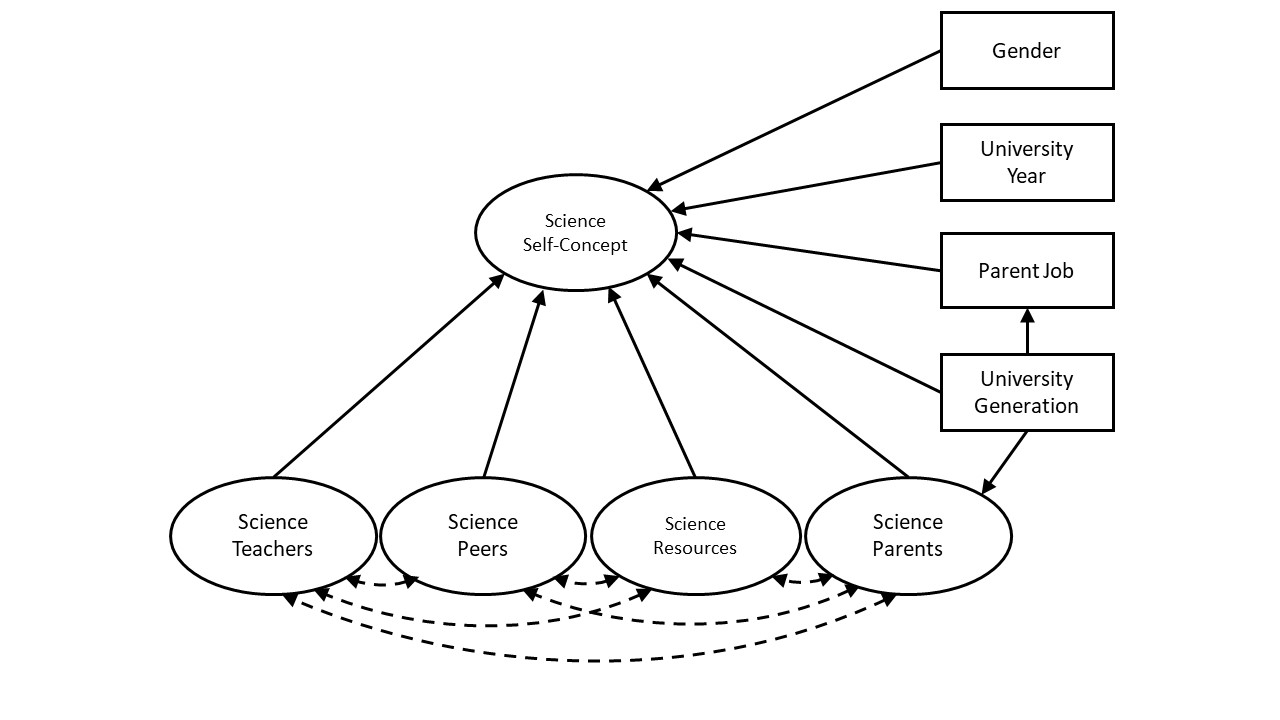
\includegraphics[width = \linewidth]{C4 - Science Capital Self-Concept/ConceptualModel.jpg}
\caption{Conceptual Model. Latent variables are represented by oval boxes, observed variables are represented by rectangular boxes. Regressions are represented by one-sided arrows, while correlations are represented by double headed arrows and dashed lines. }
\label{fig:ConceptualModel_C4}       
\end{figure*}


The following variables were included in our analyses:
\begin{itemize}
    \item \textbf{Science Self-Concept:} We included 5 items from the positive and negative self-concept scales of \cite{dewitt2011high} (``I am good at science'', ``If I study hard I will do well in science courses'').   
    \item \textbf{Science Teachers:} Experience of high school science teachers refers to the extent to which students recall having positive experiences with their high school science teachers. This scale, which included 5 items, refers to the degree of enthusiasm, care and recognition the student perceived. 
    \item \textbf{Science Parents:} Parental attitudes towards science was adapted from the parental attitudes towards science scale of \cite{dewitt2011high} and included 4 items. The item ``My parents would be happy if I became a scientist when I grow up'' was replaced with ``My parents/carers would like it if I worked in science'' to better reflect the target population.
    \item \textbf{Science Peers:} Peer value of science was measured through 4 items adapted from the ``Peer orientation towards school'' and ``Peer attitudes towards science'' scales of \cite{dewitt2011high}. One item, Q4.1 (``My friends see me as a `science' person''), did not load on to the construct. It is likely that this construct represents the participants view of their peers, as opposed to the students' subjective experience of their peers perception of them.
    \item \textbf{Science Resources:} Students' access to resources was adapted from \cite{dewitt2011high} and included 5 items. To suit our target audience, we replace the original phrase ``How often do you do the following things when you are NOT in school...'', with ``Growing up, how often did you...''. One item, Q5.5 (``Growing up, did you go to a lunchtime or after-school science club?'') did not load onto the construct. This may be due to the low number of students who responded positively to this question. An important point to consider is that we, as researchers, are defining science-related cultural capital in our own terms. Whilst the items used in the current study are by definition forms of capital, we acknowledge that other forms of capital exist and hold value in different socio-cultural contexts.
    \item \textbf{University Generations:} University Generations is a count score of the reported number of consecutive generations a participant's family has gone to university. First generation students receive a score of 0,  participants who report having siblings attend receive a score of 1, participants who report having parents attend university receive a score of 2, and those who reported having parents and grandparents attend receive a score of 3.
    \item \textbf{Parent's Job:} Participants were asked to state the profession of their father/male carer and their mother/female carer. The professions were classified according to the Australian and New Zealand Standard Classification of Occupations (ANZSCO), where a score of 0 is unemployed, 1 is low skilled, and 4 is highly skilled. The Parent's Job score is the maximum value of both parents' scores.
    \item \textbf{Gender}. Gender was recorded using an open text box, and then categorised according to the classification set out by Statistics New Zealand. Of the 693 students who completed the survey, only 1\% did not record a gender. 

\end{itemize}

Little's MCAR test showed that data could be considered missing completely at random ($p = .08$), although patterns of missing data showed that there was attrition bias --- questionnaire items tended to have more missing towards the end of the questionnaire. As a robustness check, all models were ran on the imputed and non-imputed datasets. We found that both sets of data had similar model fit, reliability, and relationships between variables. We proceeded to use multiple imputation in order to avoid list-wise deletion of cases with missing data and retain sample size. Missing data for the construct items were imputed using Predictive Mean Matching (PMM) using the MICE package in R \citep{buuren2010mice}, as PMM offers a suitable method for dealing with non-normal data \citep{little1988missing}. Cases that were missing scores on at least half the items from a construct (37 cases) were excluded from analysis (e.g., with a construct with 5 items, cases missing scores on 2 items would be kept, whilst cases missing scores on 3 or more items would be excluded). Mature students (those with a recorded age over 24) were also excluded (42 cases) as the measures of social and cultural capital employed are limited to the transmission of capital from parents and high school to university. A further 31 students were excluded from analysis due to missing data on non-imputable variables, such as parent's job, university generations, or gender. Imputation allowed us to retain 174 cases that would otherwise be excluded with list-wise deletion, leaving a  sample size of 583 students. 

Confirmatory Factor Analysis (CFA) was carried out to test the validity of our latent constructs. Concurrent and convergent validity \citep{campbell1959convergent} of these measures were established through CFA, and found to be at an adequate level. We used Cronbach's $\alpha$ and McDonald's $\omega$ to test internal consistency, with both providing similar reliability scores. McDonald's $\omega$ and Cronbach's $\alpha$ were adequate for all constructs ($\alpha$ ranging from .75 to .85, $\omega$ ranging from .74 to.86), except Science Self-Concept which had an $\alpha$ of 0.68 and an $\omega$ of .67. Whilst 0.70 is usually considered an acceptable level for internal consistency, it has been argued that $\alpha$ below 0.70 are not uncommon for attitudinal scales \citep{field2012discovering}. The lower internal consistency may also be due to the two negatively worded items (Q1.2 and Q1.5) which had lower loadings compared to the other construct items.

\subsection{Structural Equation Modelling}
Structural Equation Modelling (SEM) was used to analyse the conceptual model outlined in Figure \ref{fig:ConceptualModel_C4}. We chose to use SEM for several reasons. Firstly, SEM is able to consider hypothetical constructs that are not directly observable (such as self-concept). In practice, this means that we do not derive new variables from questionnaire items through a mean score or aggregated sum. Instead, SEM uses parameter estimates which consider measurement error and covariances between items. This is especially important when we may not expect our items to load on to a latent construct equally. Secondly, unlike simple regression models, SEM is able to model multiple relationships between variables. Doing so enables us to consider many statistical relationships in a single relative context. Finally, SEM is a widely used technique with established guidelines for judging the quality of models \citep{schreiber2006reporting}, and publicly available software \citep[e.g.][]{rosseel2012lavaan}.

SEM comprises two parts, the measurement model and the structural model. The measurement model shows the loadings of manifest variables onto each latent construct, while the structural model shows the interrelations between the latent constructs and other variables in the conceptual model \citep{schreiber2006reporting}. In our model, Science Self-Concept is viewed as a dependent variable, predicted by Science Teachers, Science Peers, Science Parents, and Science Resources. We also include other manifest variables as predictors, including Gender, University Generations, University Years, and Parent Job. We also model correlations between our latent constructs; in addition, University Generations is modelled as a predictor of Science Parents and Parent Job.

SEM with robust standard errors \citep{huber1967behavior,white1982maximum} was carried out on five imputed datasets using the Lavaan \citep{rosseel2012lavaan} and semTools \citep{jorgensen2018package} packages in R \citep{team2013r}. Rubin's rules \citep{rubin2004multiple} were used to pool point and standard error estimates across our imputed data sets. 

\section{Results}
\label{results}
Descriptive statistics, including means and standard deviations are summarised in Table \ref{tab:ItemMeansSDs}. Correlations between constructs, shown in Table \ref{tab:Correlations}, show that Science Self-Concept was significantly and positively correlated with each form of science capital explored in the current study. Science Self-Concept was most positively associated with Science Teachers ($r = 0.35$, $p<.001$), and most weakly correlated with Science Resources ($r = 0.16$, $p<.001$). We now detail the results of the SEM which explores the relationships between these constructs while including other factors present in the theoretical model (Figure \ref{fig:ConceptualModel_C4}).


\begin{landscape}
\begin{table}[ht]
\centering
\begin{tabular}[width = \textwidth]{clclccccc}
  \hline
 & Item Statement & Loading & Construct & N & Mean & SD & Skewness & Kurtois \\
  \hline
Q1.1 & \parbox[c]{70mm}{I understand everything in my science courses} & 0.62 & Self-Concept & 617 &68.75 & 19.73& -0.94&0.78\\
Q1.2 &   \parbox[c]{70mm}{I find science difficult} & -0.40 &  Self-Concept & 606 & 50.19 & 24.68 & -0.02&-0.78\\
Q1.3 &   \parbox[c]{70mm}{I get good marks in science tests} & 0.72 &  Self-Concept &617 & 67.50&18.06 & -0.42&0.06\\
Q1.4 &  \parbox[c]{70mm}{If I study hard, I will do well in my science courses} & 0.54 &  Self-Concept &620&86.69 &14.85	 &-1.59&3.53\\
Q1.5 &  \parbox[c]{70mm}{I am just not good at science} & -0.38 &  Self-Concept & 605& 20.41& 19.28& 0.85&-0.07\\
  \hline
Q2.1 &  \parbox[c]{70mm}{\begin{spacing}{0.8}My high school teachers recognised that I was good at science\end{spacing}} & 0.75 & Teachers &615&69.08	 &19.10 & -0.80&-0.28\\
Q2.2 &  \parbox[c]{70mm}{My high school teachers cared whether I understood science} & 0.72 &  Teachers &618&70.61 &26.34 & -0.88&0.01\\
Q2.3 &  \parbox[c]{70mm}{My high school teachers explained to me that science is useful for my future} & 0.64 &  Teachers &615&65.24&27.05 &-0.56	&-0.55	\\
Q2.4 &    \parbox[c]{70mm}{My high school science teachers were enthusiastic about science} & 0.64 &  Teachers &619	&75.74&23.70 & -1.06&0.52	\\
Q2.5 &   \parbox[c]{70mm}{My teachers have specifically encouraged me to continue with science after school} & 0.74 & Teachers &593&52.78&32.75 & -0.10&-1.23\\
  \hline
Q3.1 & \parbox[c]{70mm}{My parents/carers think science is interesting} & 0.59 & Parents &618	&70.62&	23.64	 &-0.75	&0.14  \\
Q3.2 & \parbox[c]{70mm}{My parents/carers think it is important for me to learn science} & 0.88 & Parents &619&65.73&26.46	 &-0.48	&-0.54	\\  
Q3.3 & \parbox[c]{70mm}{My parents/carers would like it if I worked in science} & 0.77 & Parents   &612&66.06&27.28 & -0.56&-0.45\\
Q3.4 & \parbox[c]{70mm}{My parents/carers have explained to me that science is useful for my future} & 0.80 & Parents & 592	&53.65	&31.64	& -0.10	&-1.16	\\  
  \hline
Q4.1 & \parbox[c]{70mm}{My friends see me as a ``science person''} & - & - &  602	&70.23&	28.11 &-0.86&-0.14\\
Q4.2 & \parbox[c]{70mm}{My friends think that science is important} & 0.91 & Peers & 615&68.61&	23.47 & -0.65&-0.03 \\
Q4.3 & \parbox[c]{70mm}{My friends think science is cool} & 0.83 & Peers &617&63.38&25.90 & -0.44&-0.48\\ 
Q4.4 & \parbox[c]{70mm}{My friends care about their university grades} & 0.40 & Peers &619&	81.10&	21.21 &-1.56&2.65 \\
  \hline
Q5.1 & \parbox[c]{70mm}{Growing up, did you do science activities (e.g., science kits, nature walks, do experiments)?}  & 0.55 & Resources& 581	&2.40&0.87 & 0.09&-0.68 \\ 
Q5.2 & \parbox[c]{70mm}{Growing up, did you read books or magazines about science?} & 0.69 & Resources &572	&2.42&1.01 & 0.03&-1.11\\
Q5.3 & \parbox[c]{70mm}{Growing up, did you look up things online about science or nature?} & 0.69 & Resources &592&2.97&0.97 &-0.54&-0.79	\\
Q5.4 & \parbox[c]{70mm}{Growing up, did you watch TV programmes about science or nature?} & 0.62 & Resources &599&2.89&0.91 &-0.43&	-0.64\\
Q5.5 & \parbox[c]{70mm}{Growing up, did you go to a lunchtime or after-school science club?} & - &-&579&1.50&0.93 & 1.65&	1.30\\
   \hline
\end{tabular}
\caption{Questionnaire Items. Table showing the questionnaire items used in the current study, with loadings onto the relevant latent construct where applicable. Descriptive statistics for each item are also reported. All items were scored on a continuous scale of 0--100, with the exception of Q5 items, which were scored on a Likert scale of 1-5.} 
\label{tab:ItemMeansSDs}       % Give a unique label
\end{table}
\end{landscape}

\begin{table}[ht]
\begin{tabular}{lccccc}
\cline{2-6}
                  & \parbox{16mm}{\centering Science\\ Self-Concept} & \parbox{13mm}{\centering Science\\ Teachers} &  \parbox{12mm}{\centering Science\\ Parents} & \parbox{12mm}{\centering Science\\ Peers} & \parbox{12mm}{\centering Science\\ Resources} \\ \hline
Science Self-concept  & 1                & -                & -               & -             & -                 \\
Science Teachers  & 0.35            & 1                & -               & -             & -                 \\
Science Parents   & 0.21            & 0.31            & 1               & -             & -                 \\
Science Peers     & 0.26            & 0.30            & 0.49            & 1             & -                 \\
Science Resources & 0.16            & 0.19            & 0.28           & 0.35         & 1                 \\ \hline
\end{tabular}
\caption{\textbf{Correlations between constructs for CFA.}  Variables were standardized to have a mean of 0 and a standard deviation of 1. CFA = confirmatory factor analysis. N = 583; M = 0; SD = 1.}
\label{tab:Correlations}       % Give a unique label
\end{table}


We performed a SEM analysis with robust standard errors to test the conceptual model shown in Figure \ref{fig:ConceptualModel_C4} on a sample of 583 undergraduate science students. While the hypothesized model appears to be a tolerable fit to the data (CFI = .904; TLI = .885;  RMSEA = .053, gamma-hat =  .928), model fit was improved with the inclusion of two modifications. Specifically, we added two additional correlations between items Q2.1 (``My high school teachers recognised that I was good at science'') and Q2.3 (``My high school teachers explained to me that science is useful for my future''), and items Q2.2 (My high school teachers cared whether I understood science) and Q2.4 (My  high  school  science  teachers  were enthusiastic about science). These correlations make sense theoretically, as Q2.1 and Q2.3 may point to possible expectations from teachers, and Q2.2 and Q2.4 may relate more to how personable teachers were. With these modifications, goodness of fit statistics showed acceptable model fit \citep{hu1999cutoff,steiger2007understanding} ($\chi$ = 598.38, df = 258, CFI = 0.93, TLI = 0.91, RMSEA = 0.05, SMSR = 0.05, gamma-hat = 0.95). As shown in Table \ref{tab:MeasurementModel}, the standardized loadings were all significant and acceptable. 

\begin{landscape}
\begin{table}[ht]
\centering
\begin{tabular}{llrrrrr}
  \hline
Latent & Manifest & Estimate & StandardError & z & p & Standardized \\ 
  \hline
Science Self-Concept & Q1.1 & 1.00 &  &  &  & 0.65 \\ 
   & Q1.2 & -0.80 & 0.11 & -6.99 & $<$ .01 & -0.43 \\ 
   & Q1.3 & 1.03 & 0.09 & 11.00 & $<$ .01 & 0.72 \\ 
   & Q1.4 & 0.61 & 0.07 & 8.80 & $<$ .01 & 0.55 \\ 
   & Q1.5 & -0.60 & 0.08 & -7.70 & $<$ .01 & -0.39 \\ 
  Science Teachers & Q2.1 & 1.00 &  &  &  & 0.75 \\ 
   & Q2.2 & 0.94 & 0.06 & 14.65 & $<$ .01 & 0.70 \\ 
   & Q2.3 & 0.97 & 0.08 & 12.80 & $<$ .01 & 0.72 \\ 
   & Q2.4 & 0.75 & 0.07 & 11.03 & $<$ .01 & 0.62 \\ 
   & Q2.5 & 1.18 & 0.08 & 14.51 & $<$ .01 & 0.74 \\ 
  Science Parents & Q3.1 & 1.00 &  &  &  & 0.59 \\ 
   & Q3.2 & 1.65 & 0.12 & 14.05 & $<$ .01 & 0.88 \\ 
   & Q3.3 & 1.51 & 0.13 & 12.06 & $<$ .01 & 0.77 \\ 
   & Q3.4 & 1.81 & 0.14 & 12.82 & $<$ .01 & 0.82 \\ 
  Science Peers & Q4.2 & 1.00 &  &  &  & 0.93 \\ 
   & Q4.3 & 0.99 & 0.06 & 16.26 & $<$ .01 & 0.82 \\ 
   & Q4.4 & 0.39 & 0.05 & 7.82 & $<$ .01 & 0.41 \\ 
  Science Resources & Q5.1 & 1.00 &  &  &  & 0.56 \\ 
   & Q5.2 & 1.43 & 0.11 & 12.69 & $<$ .01 & 0.69 \\ 
   & Q5.3 & 1.40 & 0.15 & 9.18 & $<$ .01 & 0.69 \\ 
   & Q5.4 & 1.16 & 0.13 & 8.84 & $<$ .01 & 0.63 \\ 
   \hline
\end{tabular}
\caption{\textbf{Measurement Model}. The measurement model summarises the loading of items onto theoretical constructs outlined in Figure \ref{fig:ConceptualModel_C4}. The results of the measurement model show that items loadings were significant and acceptable}
\label{tab:MeasurementModel}       % Give a unique label
\end{table}
\end{landscape}

The structural model, shown in Table \ref{tab:StructuralModel} and visualised in Figure \ref{fig:ConceptualModel_results_C4}, shows the interrelationships of the latent variables (specifically the impact of constructs on Science Self-Concept) and the other observed variables in our conceptual model. Results of the structural model show that Science Teachers had the most impact on students' Science Self-Concept with a significant standardised estimate ($\beta$) of 0.33. Of the other science capital related constructs, Science Peers was the only other significant predictor of Science Self-concept ($\beta =$ 0.16). For the other predictors in our model, the number of university generations in the family (Uni Generations) and identifying as male positively predicted Science Self-concept ($\beta =$ 0.12 and $\beta =$ 0.17 respectively). The number of years a student reported being at university (Uni Years) was a significant negative predictor of Science Self-Concept ($\beta =$ -0.10). 

\begin{landscape}
\begin{table}[ht]
\caption{Structural Model} 

\centering
\begin{tabular}{llrrrrr}
  \hline
 Regressions &  & Estimate & Standard Error & z & p & Standardized $\beta$ \\ 
  \hline

  Science Self-concept & Science Teachers & 0.21 & 0.04 & 5.78 & $<$ .01 & 0.33 \\ 
   & Science Parents & -0.02 & 0.06 & -0.42 & .68 & -0.03 \\ 
   & Science Peers & 0.10 & 0.04 & 2.66 & $<$ .01 & 0.16 \\ 
   & Science Resources & -0.04 & 0.18 & -0.22 & .82 & -0.02 \\ 
   & Parent Job & 0.13 & 0.10 & 1.23 & 0.22 & 0.07 \\ 
   & Uni generations & 0.15 & 0.07 & 2.3 & 0.02 & 0.12 \\ 
   & Male & 0.46 & 0.12 & 3.67 & $<$ .01 & 0.17 \\ 
   & Uni Years & -0.13 & 0.06 & -2.28 & 0.02 & -0.10 \\ 
  Science Parents & Uni generations & 0.25 & 0.06 & 4.10 & $<$ .01 & 0.19 \\ 
  Parent Job & Uni generations & 0.21 & 0.03 & 7.14 & $<$ .01 & 0.32 \\ 
  \hline
Covariances &  &  &  &  & &  \\ 
  \hline
  Science Parents & Science Peers & 1.42 & 0.19 & 7.4 & $<$ .01 & 0.48 \\ 
  Science Teachers & Science Parents & 0.96 & 0.16 & 6.02 & $<$ .01 & 0.35 \\ 
  Science Parents & Science Resources & 0.17 & 0.04 & 4.00 & $<$ .01 & 0.25 \\ 
  Science Teachers & Science Peers & 1.35 & 0.23 & 5.90 & $<$ .01 & 0.31 \\ 
  Science Peers & Science Resources & 0.37 & 0.06 & 5.82 & $<$ .01 & 0.35 \\ 
  Science Teachers & Science Resources & 0.19 & 0.06 & 3.40 & $<$ .01 & 0.20 \\ 
   
   \hline
\end{tabular}
\caption{\textbf{Structural Model}. The structural model summarises the inter-relationships between the constructs identified in the measurement model (Table \ref{tab:MeasurementModel}) and the other variables included in the theoretical model (Figure  \ref{fig:ConceptualModel_C4}). The results of the structural model show that while all of the science capital related constructs (Science Teachers, Science Peers, and Science Resources) are positively and significantly correlated, Science Teachers and Science Peers were the only significant predictors of Science Self-Concept. Of the other variables included in the model, the number of university generations in the family (Uni Generations) and being male (Male) positively and significantly predicted Science Self-Concept. The number of years a student had attended university negatively and significantly predicted Science Self-concept. These results are visualised in Figure \ref{fig:ConceptualModel_results_C4} }
\label{tab:StructuralModel}
\end{table}
\end{landscape}

\begin{figure*}
 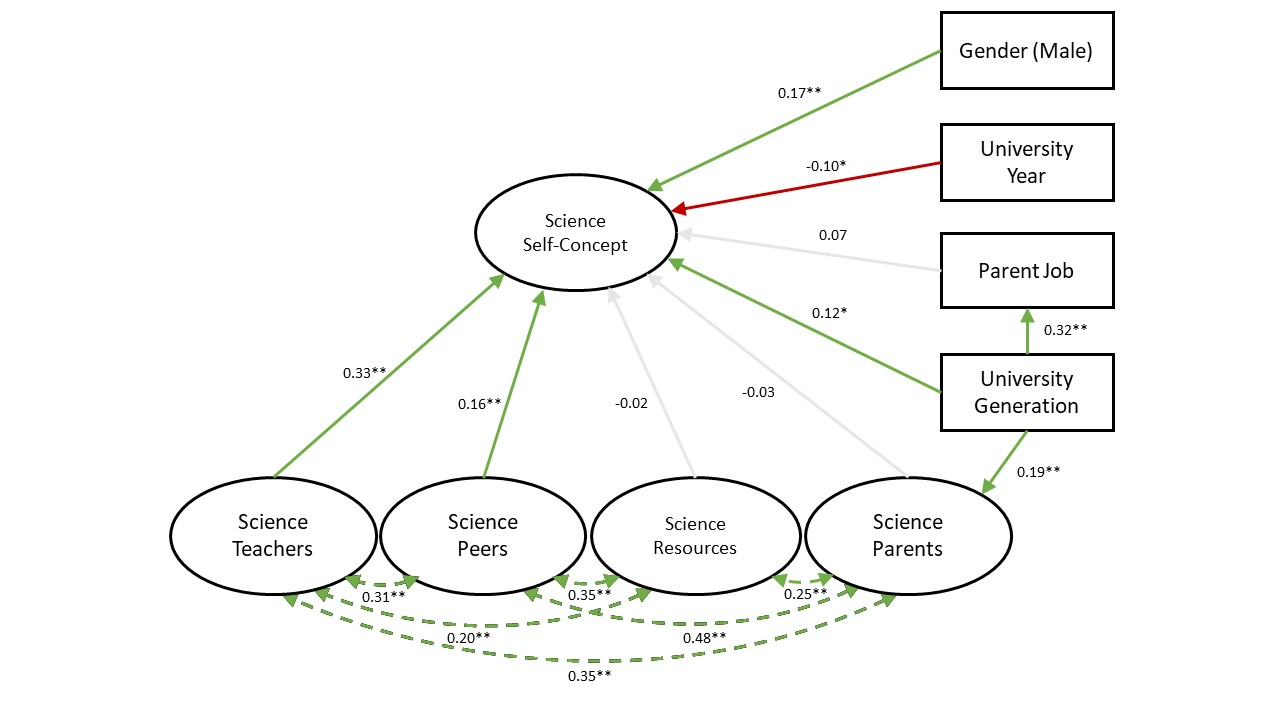
\includegraphics[width = \linewidth]{C4 - Science Capital Self-Concept/ConceptualModel_results.jpg}
\caption{Model results. Results with standardised coefficients and significant of the original conceptual model outlined in Fig \ref{fig:ConceptualModel_C4}. Single headed solid lines indicate a regression, while double headed dotted lines indicate a correlation. Green arrows indicate a positive association, while red indicates a negative association. Faded grey lines indicate no significant relationship. *$p <.05$, **$p <.001$}
\label{fig:ConceptualModel_results_C4}       
\end{figure*}

\section{Discussion}
\label{discussion}
Our results show that, while social capital and cultural capital in science are all positively associated with the science self-concept of university science students, the social relationships shared with teachers and peers are the most important. For university science students, parents' value of science and the science related resources students had while growing up were non-significant predictors of science self-concept. However, the number of university generations within the family did positively predict students' science self-concept. Results also show that male students tended to have higher levels of self-concept, and students who had attended university for more years had lower levels of self-concept. We now discuss these results in the context of university study and New Zealand science education.

Experiences with high school science teachers was the strongest predictor of science self-concept for our sample of university students. While positive experiences were linked to increased science self-concept, negative experiences predicted lower self-concept. Previous research suggests that reflected appraisals from significant others, such as those from teachers, play an important role in the way we view ourselves \citep{bong2003academic}. Tying in with Bourdieu's theory, an individual's habitus is informed by the evidence they see in the field they are participating in. Being recognised as someone who can be successful in science, by a teacher, gives students evidence that they belong. On the other hand, students who have teachers who do not appear to care about them, and who do not encourage them, may internalise the idea that science is not for them. 

The current study was cross-sectional, which means that it may also be the case that students who have low self-concept in science were less likely to have been encouraged by teachers. With that being said, research shows that teachers influence the interests of their students through the support they show students across education levels \citep{marjoribanks2006adolescents}. This process starts as early as primary school \citep{fauth2014student} and through high school \citep{marjoribanks2006adolescents,Hazari2017}. In the field of physics for example, the importance of being recognised as good at physics by teachers has been linked to increased intentions to pursue a career in the field \citep{Hazari2017}. Previous research also shows that students who experience high school teachers who are enthusiastic are more likely to be positively predisposed to the field \citep{keller2017impact}. The current research builds on previous findings by suggesting that positive high school science teachers can positively impact on the self-concept of their students after they leave high school and attend university. Teachers are thus integral to providing safe, inclusive educational environments that are recognised as important for young peoples' well-being \citep{wellbeing2019}. 

Peers' value of science was also positively associated with an individual science self-concept. The mechanism by which friends' value of science has an influence may be linked to social capital. As outlined by \cite{lin1999building}, the value of social capital is not just derived from knowing individuals who can provide access to a broader range of resources and a flow of information. Social capital also helps to build an individual's identity through shared group norms. As suggested by \citet[p.29]{Adler2017}: ``Strong social norms and beliefs\ldots encourage compliance with local rules and customs''. Self-concept may be boosted for students who have more opportunities to talk to others about science in general \citep{Archer2015a}, while receiving increased support from friends \citep{bissell2009role} and/or belonging to a network of friends at university can have positive impacts on persistence \citep{thomas2000ties}. Through a Bourdieusian lens, having a friendship group where students can act out science safely and productively may signal to a student that they belong in science. Students without the same network of support may be less likely to persist in university study \citep{thomas2000ties}. 

It is also likely that individuals with high levels of self-concept in science seek out friends with similar interests. Homophily, the idea that ``birds of a feather flock together'' \citep{mcpherson2001birds}, is a common characteristic of friendship networks. In the case of the current study, students were asked to rate the degree to which their friends think science is important, think science is cool, and care about their university grades. It may be that individuals who responded positively to these items also shared these views previously and formed friendships based on these interests. The social comparisons that students make are also an important source of self-concept \citep{butz2015salient}. Engaging with peers who hold science in high regard and making positive social comparisons to these individuals may be a source of self-concept. Individuals with low levels of self-concept in science may avoid individuals who show great interest in science as social comparisons could make them uncomfortable \citep{bong1999comparison}. The current study is unable to untangle the direction of the relationship between science self-concept and friendship choice, but provides support for future research to investigate this area.   

Parental attitudes regarding science and parental job level were found to have no significant impact on science self-concept. Given research suggests that parent-related factors may impact on adolescent students' academic self-concept \citep{fan2010effects}, we may have expected parents value of science to also positively impact on university students' self-concept in science. However, the impact of family-related variables tends to diminish as students progress through stages of education \citep{holm2011dealing}, and the current study specifically focused on university students which is a late educational stage. It is likely that all three of the family-related factors measured in the current study had a relatively greater impact during earlier stages of a student's educational journey. Whilst parents' value of science likely played a role in the interest that students have in science \citep{archer2013aspires}, parents' values are less likely to play a role in students' science self-concept judgements. The value of social capital is contingent on the context of the task that is being achieved \citep{Adler2017}. As science self-concept is specific to the field of science education, it is reasonable to assume that parents' influence is not as important as teachers and peers who are active actors in the field. Parental attitudes towards science may be more predictive of early interest or engagement in science.  

In contrast to the results for parental attitudes, the number of generations of a student's family that attended university was positively and significantly associated with students' science self-concept. The significance of the number of generations of the student's family who attended university may be related to Bourdieu's concept of cultural reproduction \citep{Dimaggio1982}. The values of parents are transmitted to their children and inform the development of habitus. Students who have university educated parents may be more likely to feel `at home' in a university field. For first generation students, the breaking of new ground may be more confronting and challenging mentally \citep{gardner2011those}. In psychological terms, the internalisation of the idea that ``if my family can do it, so can I'', corresponds to Bandura's \citep{bandura1986explanatory} idea of establishing self-concept through vicarious experience. Seeing someone experience success who is similar to you (i.e., family) may have an especially strong impact on self-concept. With regards to the student's habitus, vicariously experiencing success would help students internalise the idea that university is for \textit{them}. Alternatively, university educated parents may also improve the academic performance of students \citep{paul2011cultural}, which in turn may influence science self-concept. Having family members who attended university is also an important form of social capital, in that it provides students with knowledge on the rules of the field, and what is needed to be successful.

The level of a student's science-related resources growing up, or objectified cultural capital, was found to be non-significant relative to the other factors included in our analysis. It may be that the resources investigated have more importance in generating early interest in science, while students in our sample were already at university. Reading about science and looking things up online about science may relate more strongly to a student's broader interests in science as opposed to their self-concept or self-belief. It may also be that students' social relationships with their teachers and peers (which both positively impacted in self-concept) ameliorate any detrimental effects that a lack of resources would have. The questionnaire items used in this study asked students to recall their access to science-related resources growing up. Future studies should seek to employ a longitudinal research design to more accurately capture the impact of resources on future self-concept in science. 

Students' self-reported gender was significantly related to science self-concept, such that male students, controlling for all other factors, reported higher levels of science self-concept than female students. The lower levels of science self-concept for female students is a common finding in STEM education research \citep{sax2015but,Ellis_2016}. Research has found that students (both male and female) tend to be more likely to make external attributions for a man's failure in science (i.e., the reason for failure is not due to lack of ability, but a poor test or bad luck), but are more likely to attribute women's failure to internal sources (lack of ability) \citep{LaCosse_2016}. 

In a Bourdieusian framework, gender differences in science self-concept can be explained in terms of a `gendered' habitus, a variation of classed habitus \citep{Reay_2004}. This relates to the idea that if individuals are exposed to ``homogenous conditions of existence imposing homogenous conditionings'' individuals will generate ``homogenous systems of dispositions'' \cite[p.101]{Bourdieu1984}. In more basic terms, if individuals are exposed to similar socio-cultural norms and environments, they may be more likely to share similar dispositions. While science has historically been a domain in which men have opportunities to succeed, women face explicit and implicit obstacles \citep{cheryan2017some,Blickenstaff_2005}. These include pervasive negative gender stereotypes \citep{Nosek_2009}, and unfair judgements regarding competency \citep{Moss_2012,Barthelemy_2016}. Men may be more likely to internalise the idea that science is a domain where they belong and can perform, and this may explain why male science students are more likely to hold higher levels of self-concept in science compared to female science students. Although the effect of gender on science self-concept was relatively small, the findings of the current study support the arguments set out by \cite{Kost_Smith_2010} who suggest that the attrition of female students from STEM domains is the result of many small effects that contribute to a ``smog of bias'' where men are bolstered and women face obstacles. 

Finally, the number of years a student reported being at university was found to negatively predict science self-concept. There is a lack of previous research investigating the temporal nature of self-concept in science at university, although one study of a mixed university sample found that academic self-concept may decrease after the first year \citep{isiksal2010comparative}. Other research has found that STEM students' self-efficacy does not decrease from first year to graduation, with it increasing for female students and remaining stable for male students \citep{macphee2013academic}. With regards to the current study, it may be that as students progress through science at university, course content becomes more challenging and thus students may be more likely to report finding science more difficult. Future research should adopt a longitudinal research design to investigate temporal changes in science self-concept in more detail. 

\section{Implications}
The current study provides insights into factors that are related to university students' self-concept in science. The findings reported may inform researchers and policy makers on the cultural and social forms of capital that are required to produce confident learners in science. The current study finds that, for students studying science at university, the social relationships that they have are especially important.

The current study highlights the important role that high school science teachers play in boosting the self-concept of university students. Our results suggest that the impact of high school science teachers continue to be manifested in students' self-concept even after high school is finished and students have entered into university study. Given the importance of self-concept in future achievement \citep{uccar2017role,chang2008science}, the results of the current study suggest that increased teacher support provides a clear method of meeting government aims for increasing the number of skilled workers in science. Massive Open Online Courses (MOOCs) are often cited as a possible solution for teacher shortages, increasing access to education when opportunities are otherwise limited. We argue that even if MOOCs are used, they must still provide students with social connections to teachers who can provide them with real, tangible feedback and recognition. The student-teacher bond should also be the targeted source of intervention to address equity issues in science \citep{banerjee2016systematic}. The expectations that teachers hold for their students may be particularly important \citep{rubie2006teacher}. Research suggests that teacher expectations are an important predictor of students transition to university study, especially for students from low SES backgrounds \citep{gregory2013takes}. 

Our findings also suggest that social relationships with peers who hold science in high regard are linked to science self-concept. This result is especially important to consider for students who originate from social groups that are underrepresented in science and may find it more difficult to form social bonds with other students. Institutional support networks, such as Women in Science, and other community building equity programmes can play an important role in connecting underrepresented students with one another, and help to build a scaffold of peer support \citep{ong2018counterspaces}. Our results also bring attention to the need to ensure that students who are the first generation in their family to attend university are adequately supported in their learning.  

\section{Limitations}
The current study, whilst providing new insights into the factors affecting self-concept of university science students in New Zealand, does have limitations that future studies should seek to address. The questionnaire, short in duration, offered insights into a select group of factors that have been found to be associated with science participation and achievement. The original questionnaire designed by \cite{dewitt2011high} had many other factors that included, but were not limited to, science aspirations, views of scientists, and parental involvement. Furthermore, given the anonymous nature of the questionnaire, it was not possible to link survey responses to administrative data that could give an indication of students' prior or future achievement, and self-reported measures of achievement contained too much missing information to be useful. Prior achievement is likely to account for much of a students' science self-concept and needs to be considered in the context of the current findings.

The sample of students who responded to the survey also display survivorship bias. These are students who have already demonstrated interest and a certain level of success in science. Our study does not account for students who dropped out of science before university. While this may be viewed as a limitation, it also focuses the current study on an \textit{asset-based} framework instead of deficit models of student outcomes. Given our sample of students all demonstrated a certain level of success, we focus on factors that were particularly important for students who made the transition to university science education. Our sample and study design also allows us to identify students who are underrepresented in science based on their demographics or access to capital, but who still recorded high levels of self-concept. A follow-up study will employ a qualitative approach to understand the experiences of these students and refine the directions of future research.

While not reported in our results, our analysis did not find sufficient evidence of measurement invariance across subject disciplines, which suggests that the constructs and relationships outlined in our conceptual model may differ for students by subject. This is not surprising, given the sample sizes per discipline and our generalised measure of science self-concept. Nevertheless, these preliminary results of the SEM suggested that, for our sample, different forms of capital may carry different value across fields, a finding inline with Bourdieu's theory. Each field has its own unique perspective on what forms of capital are valued. While the more general science related factors explored in the current study were found to be associated with a general self-concept in science, specific forms of capital may be particularly important in each science sub-field. For example, mathematics knowledge and self-efficacy in calculus may be more important for students studying in physics \citep{Black2016,Ellis_2016}. More research is needed to identify, summarise, and test the forms of capital that are valued in each science domain. We recommend more in-depth and tailored questionnaires are administered to students per subject discipline.  

\section{Conclusion}
The current study investigated the influence of science-related cultural and social capital (science capital) on the science self-concept of undergraduate science students at the University of Auckland. A Structural Equation Model (SEM) was used to explore the relationships between a set of latent constructs defining science capital and observed measures, such as university generations in the family, parents' employment, and self-identified gender. Our theoretical model provided a good fit to our data, and gives some new insights into the relationship between science capital and science self-concept. We found that, for the students in our sample, positive experiences with high school science teachers was the most important predictor of science self-concept, whilst having peers who value science was also found to be important. Interestingly, we found that reported science-related resources and parents' value of science were not significant predictors of science self-concept, but the number of university generations in the family did have a positive association. These results provide an example of how family culture reproduced over generations may manifest as students' self-belief in the field of university science education. Finally, we also found that students who self-identified as male had higher levels of science self-concept, even after accounting for social and cultural factors in our theoretical model. We discussed these findings in the context of a growing body of research regarding equity in the field of science education, and in the context of Pierre Bourdieu's sociological theory.  

\section{Author Contributions}

SMT, KM, KL, and DO contributed conception and design of the study; SMT administered the questionnaire and organized the database; SMT performed the statistical analysis; SMT wrote the first draft of the manuscript; All authors contributed to manuscript revision, read and approved the submitted version.

%\bibliography{C4 - bib.bib}













 
\chapter{Understanding Capital Accumulation in University Science}

\section{Preamble}
Following our analysis of broad level patterns in science enrollment in chapters 1 and 2, I sought to go deeper into the question of \textit{why} these patterns exist. Through analysis of the survey, we can now see how different forms of capital may influence the way students see themselves in science. The conceptual model used in Chapter 4 is however, relatively simplistic and linear. The simplicity is in part due to the constraints in the survey data collected (as it was cross-sectional) and in the survey tool itself (can we even measure habitus?). As described by Bourdieu, capital and habitus \textit{interact} and build on each other. One piece of minor feedback I received from PLoS ONE upon the submission of the article from Chapter 2 was that the interaction of capital and habitus was not sufficiently captured in the illustration of the conceptual model, but that this may be the topic a separate paper. The following chapter seeks to build my conceptual model further. This section was written following a deductive analysis of interview data that will be presented in the following chapter. The model, whilst completely based on Bourdieu's original theory, provides a new way of visualising the reciprocal relationship between capital and habitus. The model outlined and described presently will be used to interpret student experiences in university science, and also to point to opportunities for intervention. 


\section{Introduction}
The goal of this chapter is to build a theoretical model, based on Bourdieu's sociology, that may help us understand students' experiences of university science education. More specifically, the model seeks to describe the reciprocal relationship shared between students' internal dispositions (habitus) and their social relationships (social capital). The following sections will describe, step by step, the manner in which social capital relates to habitus, and how habitus directs future accumulation of capital. Using examples from the field of university science education, this paper also describe how each of the six component parts of the theoretical model may be targeted to address equity issues in university science education.

\begin{figure}[ht]
\centering
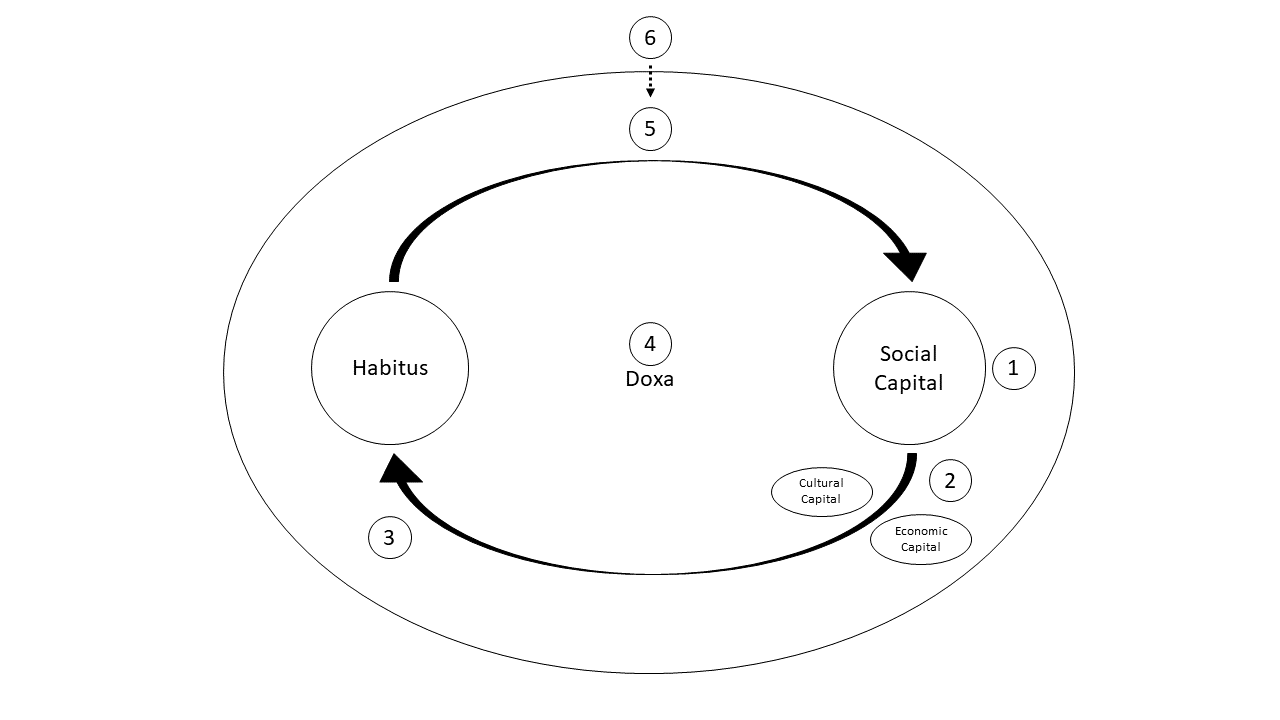
\includegraphics[width=\textwidth]{C5 - Understanding Capital Accumulation/HabitusSocCap_TheoreticalModel.png}
\caption{\label{fig:TheoreticalModel_C5}\textbf{Complete Theoretical Model}. The complete theoretical model. The model, informed by the described experiences of university science students, expands on the interaction between habitus and capital originally illustrated by \cite{Bourdieu1984}. The model provides a step by step description of how social capital translates into habitus transformation, and how habitus generates future capital accumulation. Step 1 refers to the initial availability of social capital for an individual. Step 2 refers to the value gained through leveraging social capital into forms of economic and cultural capital. Step 3 refers to how social capital is internalised by the individual. Step 4 refers to how habitus informs the acquisition of future social capital. 5 refers to factors outside of the individual that structure the field (by availability of capital and exchange value).}
\end{figure}

\section{Social Capital in the Field of University Science (Step 1)}
This section discusses the availability of social relationships that participants had in the field of university science (Figure \ref{fig:TheoreticalModel1_C5}). These relationships are categorised into three key groups, social capital through family connections, social capital through lecturers, and social capital through peers. 

\begin{figure}[h!]
\centering
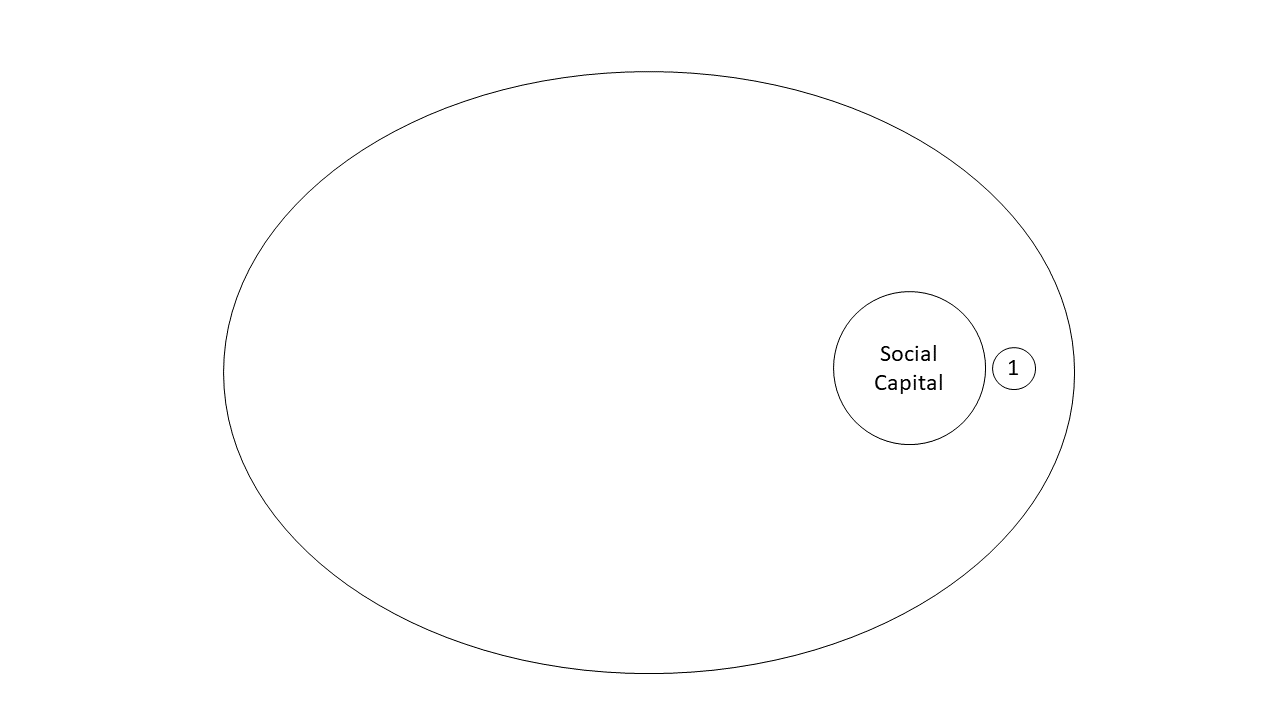
\includegraphics[width=\textwidth]{C5 - Understanding Capital Accumulation/HabitusSocCap_TheoreticalModel1.png}
\caption{\label{fig:TheoreticalModel1_C5}\textbf{Step 1}. The first step of the theoretical model. Step 1 refers to the initial availability of social capital for an individual.}
\end{figure}

The relationships that students share have been found to be important factors in success in university science. Research has shown that increasing access to mentors can improve outcomes for undergraduate students in the life sciences \citep{aikens2016social}. 


\section{Leveraging Social Capital (Step 2)}
The value of social capital is derived from the economic and cultural capital that can be mobilised through connections with others (Figure \ref{fig:TheoreticalModel2_C5}). These resources may provide students with advantages in supporting their learning and providing student access to information about the field. 

\begin{figure}[ht]
\centering
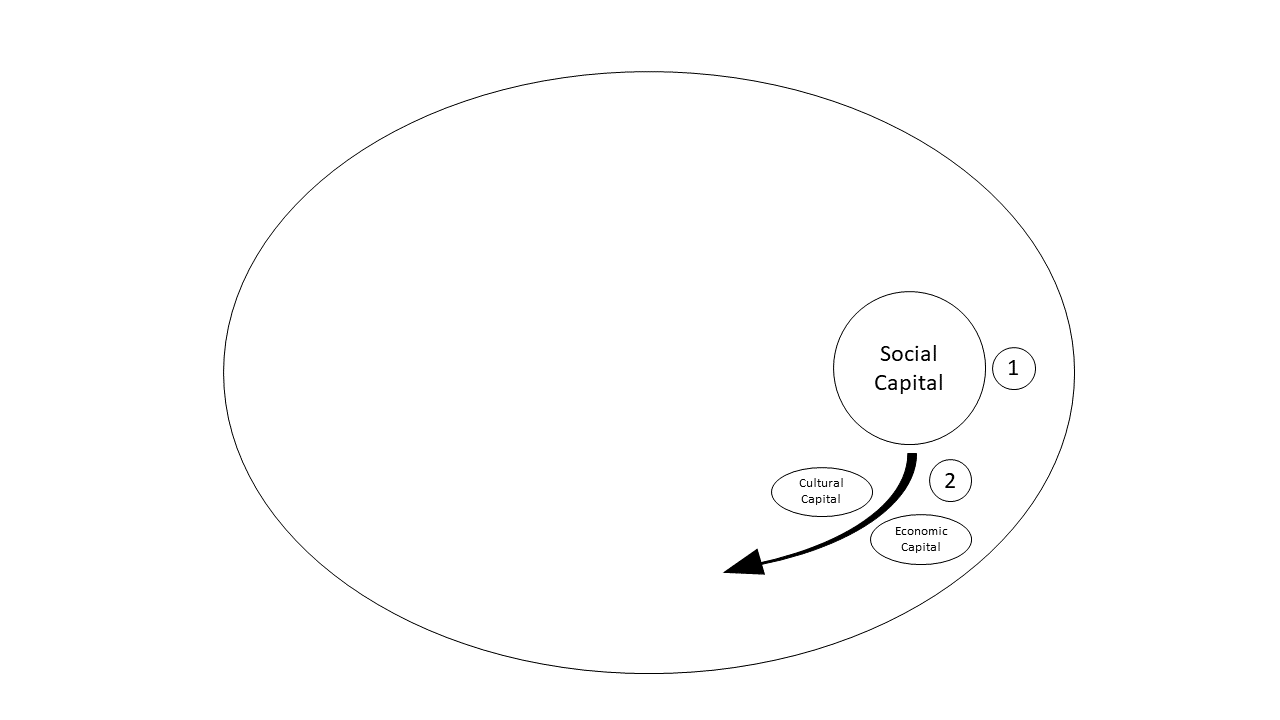
\includegraphics[width=\textwidth]{C5 - Understanding Capital Accumulation/HabitusSocCap_TheoreticalModel2.png}
\caption{\label{fig:TheoreticalModel2_C5}\textbf{Step 2}. The second step of the theoretical model. This step refers to the utility of social capital in mobilising cultural capital and economic capital.}
\end{figure}

Inequities in science education outcomes exist not only in the access individuals have to capital, but also in the value that society places on the capital that different groups hold. In the field of science, a wealth of research has shown that value is often defined by the terms of those who have historically held power in the field. Across gender, ethnicity, social class, sexual orientation, and disability, those who are less well-represented are more likely to feel out of place and marginalised. 


\section{Internalising Capital (Step 3)}
The capital that students accrue in university science not only provides access to resources, but it can also influences the way that students see themselves in the field. Capital, which determines students position in the field, is internalised by students via their habitus  (Figure \ref{fig:TheoreticalModel3_C5}), which establishes the students disposition towards the field \cite{Bourdieu1992}. Students who hold high levels of social capital may feel an affinity with the field and see progression to university as a path already drawn out.

The process of socialisation.
The process of objectified cultural capital transforming into embodied cultural capital (physical and mental - habitus)

\begin{figure}[ht]
\centering
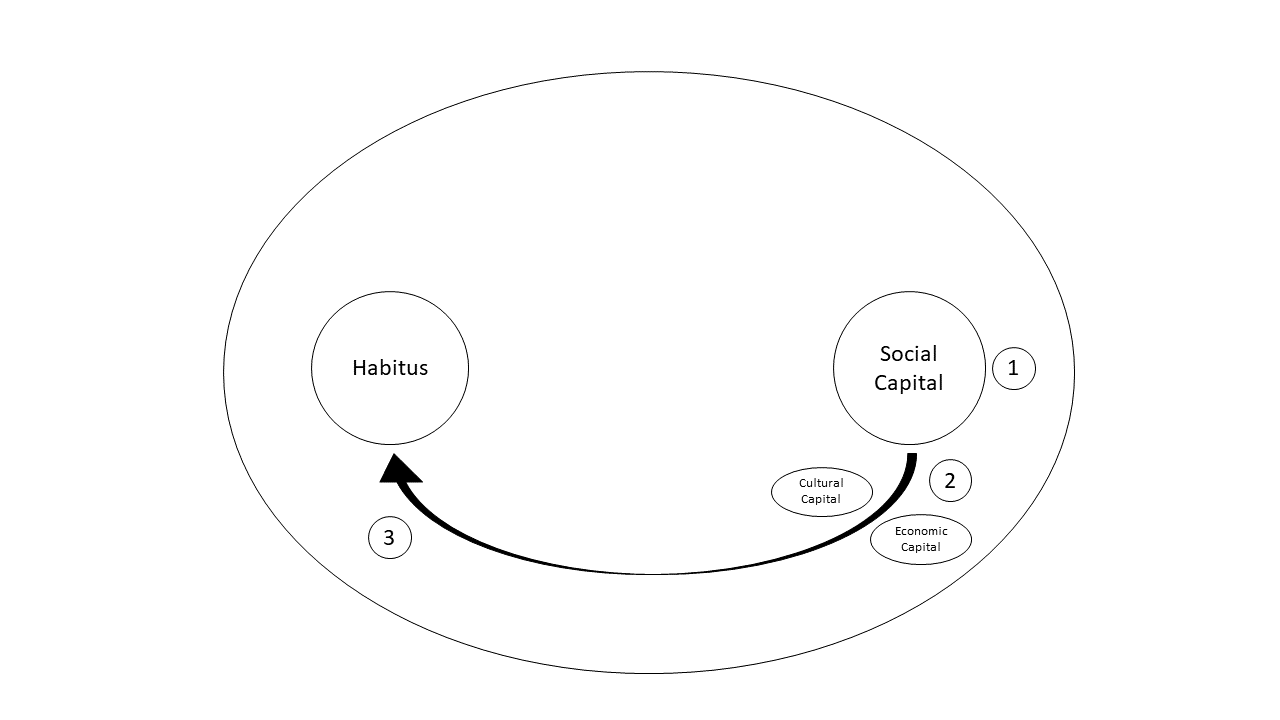
\includegraphics[width=\textwidth]{C5 - Understanding Capital Accumulation/HabitusSocCap_TheoreticalModel3.png}
\caption{\label{fig:TheoreticalModel3_C5}\textbf{Step 3}. The third step of the theoretical model. This step refers to the manner in which capital is internalised by individuals via habitus.}
\end{figure}



\section{Doxa (Step 4)}
Outside of the of the social relationships that students hold, general discourses in society influence the development of habitus (Figure \ref{fig:TheoreticalModel4_C5}). 

Bourdieu uses the term ``classed habitus'' to refer to the way in which members of the same social group are exposed to similar experiences and thus have similar dispositions and lifestyle practices. The concept of classed habitus has since been used in research in terms of gendered habitus \citep{Reay_2004}, Chinese habitus \citep{Mu2014}. Theorists advocating for intersectional approaches to identity research argue that experiences may be vastly different for individuals based on. For example, research shows that women of colour face many different barriers to success in the field of physics \cite{ong2005body}.

\begin{figure}[ht]
\centering
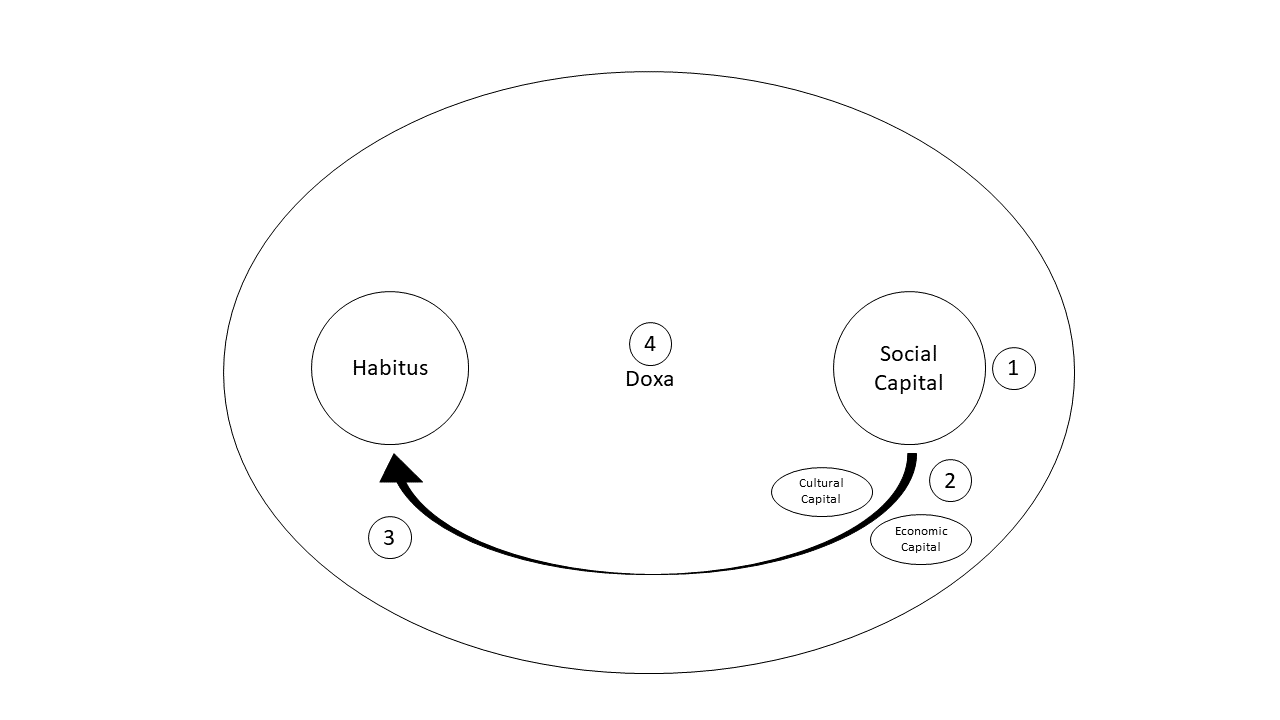
\includegraphics[width=\textwidth]{C5 - Understanding Capital Accumulation/HabitusSocCap_TheoreticalModel4.png}
\caption{\label{fig:TheoreticalModel4_C5}\textbf{Step 4}. The fourth step of the theoretical model. This step refers to the impact doxa (pervasive societal discourses) has on students' habitus.}
\end{figure}

\section{Generating Social Capital (Step 5)}
The future acquisition of social capital is informed by habitus (Figure \ref{fig:TheoreticalModel5_C5}). 

Students who lack capital entering into university may need to make sacrifices to other aspects of their life to get ahead. 

\begin{figure}[ht]
\centering
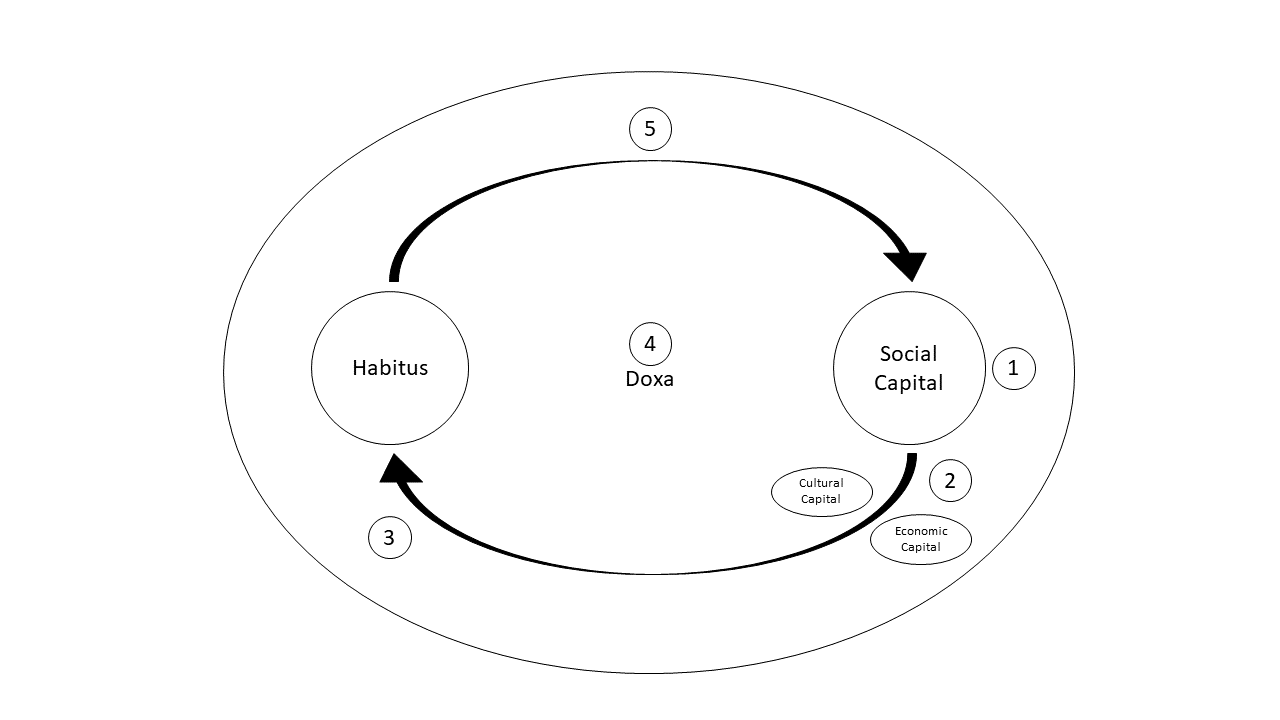
\includegraphics[width=\textwidth]{C5 - Understanding Capital Accumulation/HabitusSocCap_TheoreticalModel5.png}
\caption{\label{fig:TheoreticalModel5_C5}\textbf{Step 5}. The fifth step of the theoretical model. This step refers to the manner in which students' habitus directs the future acquisition of social capital}
\end{figure}



\section{Institutional Habitus (Step 6)}
The cycle is impacted on by interventions operating in the field, which themselves are directed by an institutional habitus (Figure \ref{fig:TheoreticalModel6_C5}). 

\begin{figure}[ht]
\centering
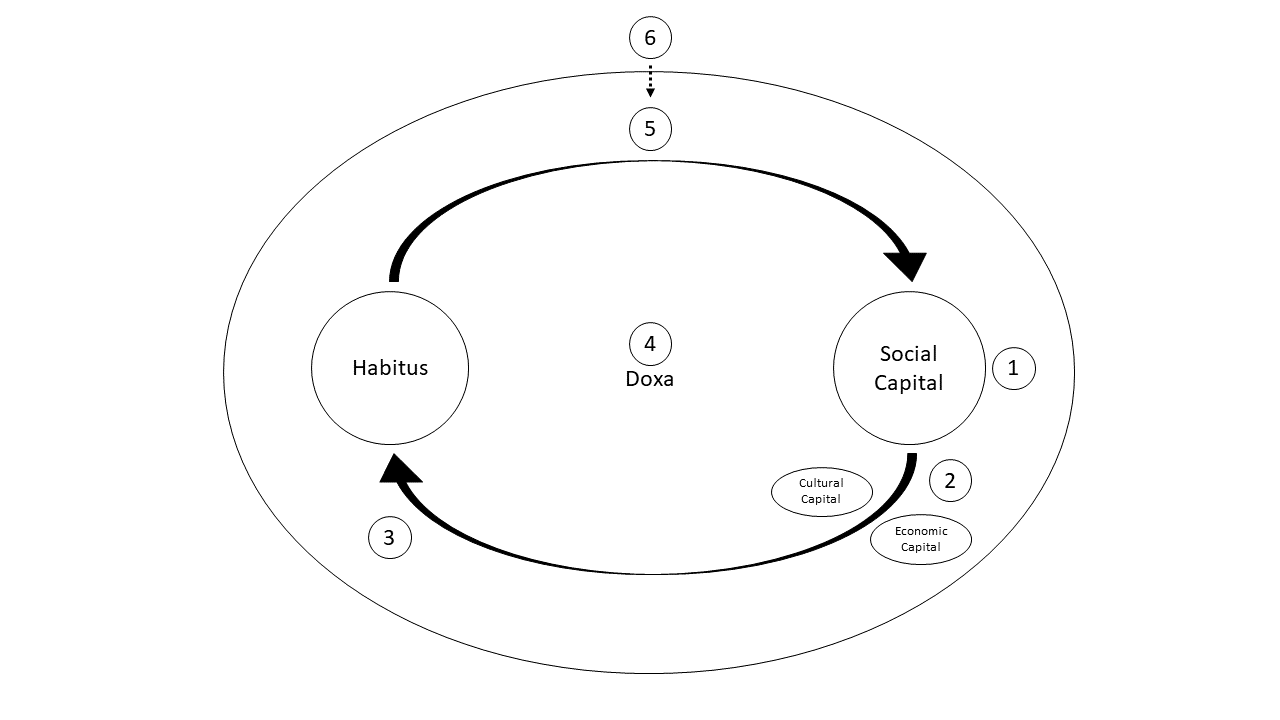
\includegraphics[width=\textwidth]{C5 - Understanding Capital Accumulation/HabitusSocCap_TheoreticalModel.png}
\caption{\label{fig:TheoreticalModel6_C5}\textbf{Step 6}. The sixth step of the theoretical model. This step refers to the manner in which institutions impact on the cycle}
\end{figure}



\section{Conclusion}



\chapter{Experiences of Science Capital in University Science}

\section{Preamble}
The following chapter details the results of a set of nineteen interviews that were conducted with science students at the university of Auckland. I mirror the structure of the previous chapter, where I outline arguments for a conceptual model of how capital is accumulated by students as university. The current chapter, in addition to detailing the qualitative methodologies employed, will seek to add the colour of life experiences to my conceptual model. It is in this chapter where I seek more understanding of \textit{why} students do or do not choose to study science.

\subsection{Capital in the Field of University Science Education}



\subsection{Introduction}
The goal of the current chapter is to explore how the conceptual model outlined in Chapter 5 is experienced by students at the University of Auckland (UoA). More specifically, I seek to answer three specific research questions:
\begin{itemize}
    \item What forms of social capital are available to university science students? 
    \item How do students leverage social capital to gain advantage in the field of university science? 
    \item How does students' habitus contribute to the accumulation of capital?
\end{itemize}

I adopted a staggered research design, where the research process took place over three separate phases. As shown in Table \ref{tab:Phases}, the process began with four interviews with students in the science scholars programme (a programme for gifted science students) at the UoA. Based on preliminary data from these interviews and a questonnaire provided by the ASPIRES research group in the United Kingdom \citep{dewitt2011high}, a questionnaire was designed to assess the relationships between students' social capital, cultural capital, social location (gender, ethnicity, socio-economic status), and confidence in science. The questionnaire asked students to record factual information about themselves, and answer items regarding 5 latent constructs informed and adapted from the work of \cite{dewitt2011high}. The constructs included self-concept in science (Science Self-concept), experience of high school science teachers (Science Teachers), parental attitudes towards science (Science Parents), peer attitudes towards science (Science Peers), and access to science-related resources (Science Resources). Results of a Confirmatory Factor Analysis (CFA) provided support for these 5 factors ($\chi^{2} =$ 483.74, $\mathrm{df} =$ 179, p $<$ .001, CFI  $=$ 0.93, TLI  $=$ 0.91, RMSEA $=$ 0.05), while separate tests of showed adequate reliability of each construct (McDonald's $\omega$ 0.68 - 0.86). More detailed information regarding questionnaire design and quantitative results is available in Chapter 4. 
\begin{table}[ht]
\begin{tabular}{c|c|l}
                      
Phase  & Year & Purpose    \\ \hline
1   & 2018  & Interviews with 4 high achieving science students at UoA.     \\
& & Results of these interviews were used to inform questionnaire design. \\ \hline
2  & 2018-2019 & Questionnaire design and administration to science students at UoA.  \\
& & Questionnaire analysis conducted (see Chapter 4)\\ \hline
3 & 2019 & Main interviews conducted with 15 students. \\
& & These were selectively sampled from the questionnaire. \\ \hline
\end{tabular}
\caption{\label{tab:Phases} The timeline of the qualitative research process. Preliminary interviews with four high achieving science students informed the design of questionnaire, which was administered to science students at UoA in early 2019. Fifteen students were then purposefully sampled for interviews based on questionnaire responses.}
\end{table}

The current study draws from the pool of questionnaire respondents. The staggered research design has been used in previous research to investigate student experiences in STEM to great effect \citep{grossman2014perceived,russell2011factors}. Whereas previous research has focused on random sampling \cite{russell2011factors} or purposeful sampling to achieve a balance of gender or ethnicity in interviews \citep{grossman2014perceived}, the current study seeks to take a more intersectional methodological approach by including domain-specific indicators of social class as well as self-report measures of gender and ethnicity in the decision making process. As shown in \ref{fig:ScienceFactors_C6}, students were purposefully sampled from a range of different social locations, with the aim of representing a range of student experiences. Through interviews with these students, it may be possible to untangle some of the complexities that surround the impact of parents, peers, and resources on experiences of university science education. The following section will outline the methods used in the interview phases in more detail.

\begin{figure}[ht]
\centering
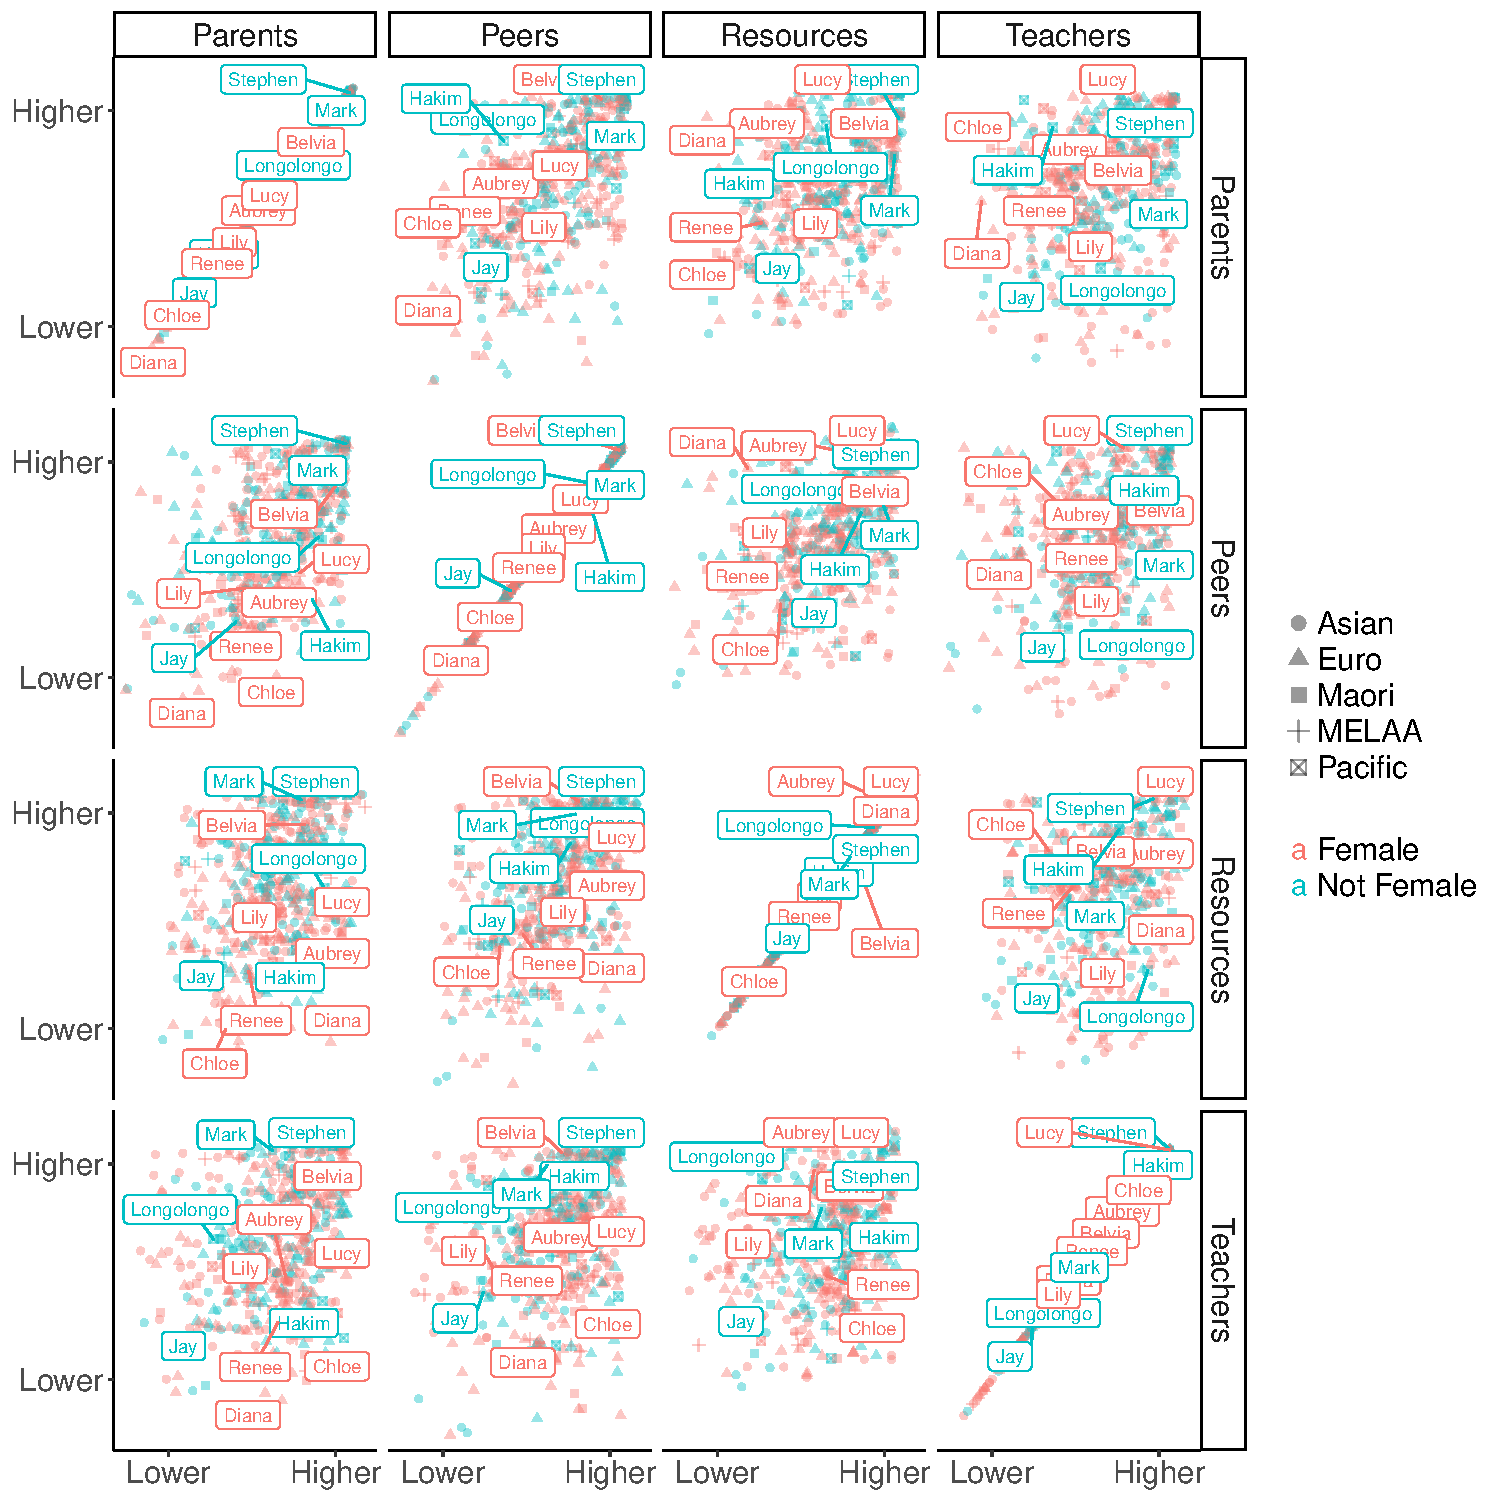
\includegraphics[width=\textwidth]{C6 - Experiences of Science Capital/ScienceFactors_FacetPlot.pdf}
\caption{\label{fig:ScienceFactors_C6}\textbf{Sampling Strategy}. The above plot shows the methods used to sample students when arranging interviews. I aimed to interview students with a range of different backgrounds with regards to forms of science capital. Axes indicate the students' level of a particular form of capital, including Science Parents, Science Peers, Science Resources, and Science Teachers. The locations of 12 of the 19 interviewee participants are highlighted by their pseudonym. The four participants interviewed at phase 1 are not included, while three interview participants from phase 3 were excluded from factor analysis due to having too much missing data in the questionnaire (see Turnbull (in review) for more details). Individual data points are also coloured and shaped at the intersection of identified gender and ethnicity. In this case, ethnicity is coded according to prioritised ethnicity, where students who identified with multiple ethnicities were first coded as M\={a}ori, then Pasifika, then Asian, then European (following guidelines set out by Statistics New Zealand). I only use the prioritised ethnicity for ease of plotting and not for any analysis. Gender in this case refers to whether the individual self-identified as female or not. }
\end{figure}

\section{Methods}

\subsection{Context}
The current study discusses data from nineteen semi-structured interviews conducted with students enrolled in STEM subjects at the University of Auckland (UoA). Four students were invited to interview based on their participation in the science scholars programme at the UoA, and fifteen students were purposefully sampled from the pool of questionnaire respondents. Given the goal of these interviews is to reveal variation in the students experiences in science, rather than to discuss the properties of a `sample', it can be argued that a sample size of 19 participants is sufficient \cite{berglund2006students}. For participants drawn from the questionnaire, sampling was prioritised based on the constructs of capital measured in the questionnaire (Figure \ref{fig:ScienceFactors}), and also according to whether they identified as a member of an underrepresented social group in science. The purposeful sampling was a deliberate choice informed by research on intersectionality. As outlined by \cite{duran2019using}: ``Even if multiple marginalized demographics are not the subject, they must always be centered.'' The social groups I intentionally sampled were thus as follows:
\begin{itemize}
    \item Individuals with lower levels of science related capital. This judgement was made based on students reported scores on the teachers and peers value of science constructs, which were found to be the most important predictors of self-concept in science in Chapter 4.  I also took into account other indicators of science-related capital, such number of books at home growing up and access to science related activities.
    \item Individuals with parents who do not value science, or who do not talk about science often. Even though parents value of science was not a significant predictor of science self-concept in Chapter 4, I expected it to still play a major role in participants' development of habitus in science. 
    \item First generation to university students. 
    \item M\={a}ori and Pasifika students. While research has explored factors relating to success at university in general for students identifying as M\={a}ori and/or Pasifika \citep{mayeda2014you}, there is a need for research that seeks to present their experiences in science specifically. 
    \item Female students in physics and computer science. Through interviews with these students we may begin to describe why we see certain trends in student enrolments, such as those described in Chapters 2 and 3.
\end{itemize}
While the above criteria represent the students of specific interest, the students interviewed represented a range of social backgrounds, with some students representing multiple criteria and some not representing any. It is also important to note that the categories employed are simplistic and do not encompass a range of other important characteristics (such as religion or ableness), or indeed the complexity of belonging to multiple groups. While much research of marginalised groups in science is grounded in deficit-theorising (why do students drop out?), the current study attempts to adopt an asset-based framework (why do students succeed?). This framing is prefaced by the acknowledgment that while resilience should be celebrated, it should not be necessary. Participant characteristics are summarised as in Table \ref{tab:Demographics} and participant summaries are also available as supporting information. 


\begin{table}[ht]
\begin{tabular}{cc|c}
                       &                        & Count \\ \hline
Gender                 & Male                   & 7     \\
                       & Female                 & 8     \\ \hline
Ethnicity              & Asian                  & 3     \\
                       & M\={a}ori                  & 7     \\
                       & Pasifika               & 3     \\
                       & Pakeha/European        & 9     \\ \hline
University Generations & First Generation       & 7     \\
                       & Sibling                & 2     \\
                       & Parent                 & 4     \\
                       & Grandparent and Parent & 2     \\ \hline
Subject Disciplines    & Biology                & 8     \\
                       & Chemistry              & 7     \\
                       & Computer Science       & 6     \\
                       & Mathematics            & 3     \\
                       & Physics                & 7     \\
                       & Psychology             & 3     \\
                       & Statistics             & 4     \\ \hline
Self-concept          & Higher                   & 7     \\
                       & Lower                    & 5     \\ \hline
Science Parents        & Higher                   & 8     \\
                       & Lower                    & 4     \\ \hline
Science Teachers       & Higher                   & 7     \\
                       & Lower                    & 5     \\ \hline
Science Peers          & Higher                   & 7     \\
                       & Lower                    & 5     \\ \hline
Science Resources      & Higher                   & 8     \\
                       & Lower                    & 4    
\end{tabular}
\caption{\label{tab:Demographics} A table summarising the characteristics of the individuals who participated in interviews following completion of the questionnaire. Aggregated group counts are provided to help preserve anonymity. Participants may have identified with multiple ethnicities or be enrolled in multiple subject disciplines, which means that these counts do not sum to fifteen. Three students who participated in interviews did not provide enough information on construct items to have scores on self-concept and capital scales attributed to them. Information is not presented for the four students who completed the first interview phase of the study, prior to administration of the questionnaire.}
\end{table}

\subsection{Qualitative approach and research paradigm}
Interview questions were based on the items presented to participants in the questionnaire. These questions reflect a deductive approach, where previously established theory guides questions. This process was conducted explicitly by using the participants' questionnaire responses as an object for discussion. For example: 
\blockquote{On this section: my friends see me as a science person. You scored quite highly - how do you feel about that?} While interviews were directed by participants' questionnaire responses, they were also semi-structured. This means that participants were invited to lead discussion and talk about what they felt was important. As M\={a}ori were invited to be interviewed, this inductive approach was informed by Kaupapa-M\={a}ori-Consistent (KMC) practices. KMC practice requires research concerning M\={a}ori to be conducted with, and not on, M\={a}ori \citep{walker2006exploration}. My attempts to adhere to KMC practices meant that the conceptualisation and operationalisation of research procedures were also discussed with M\={a}ori representatives, and that participants were offered transcripts of interviews and manuscript drafts, and invited to remove, edit, and add responses after the interview.  

An inductive approach to thematic analysis was used to analyse the interview transcripts, following the general guidelines set out by \cite{Braun_2006}. Interviews were coded in accordance to the the three established research questions:  what forms of social capital are available to university students? How do students leverage social capital to gain advantage in the field of university science? And finally, how does students' habitus contribute to the accumulation of capital? Themes were then established and developed into the conceptual model outlined in Chapter 5 to aid in answering these questions. Bourdieu's sociological theory was employed as a conceptual ``toolbox'', drawing primarily on his concepts of social capital, habitus, field and doxa. The conceptual model (Figure \ref{fig:HabitusSocCap_TheoreticalModel_C6}) provides a lens to explore how social capital impacts on habitus, and how habitus then influences future capital accumulation. 

\begin{figure}[ht]
\centering
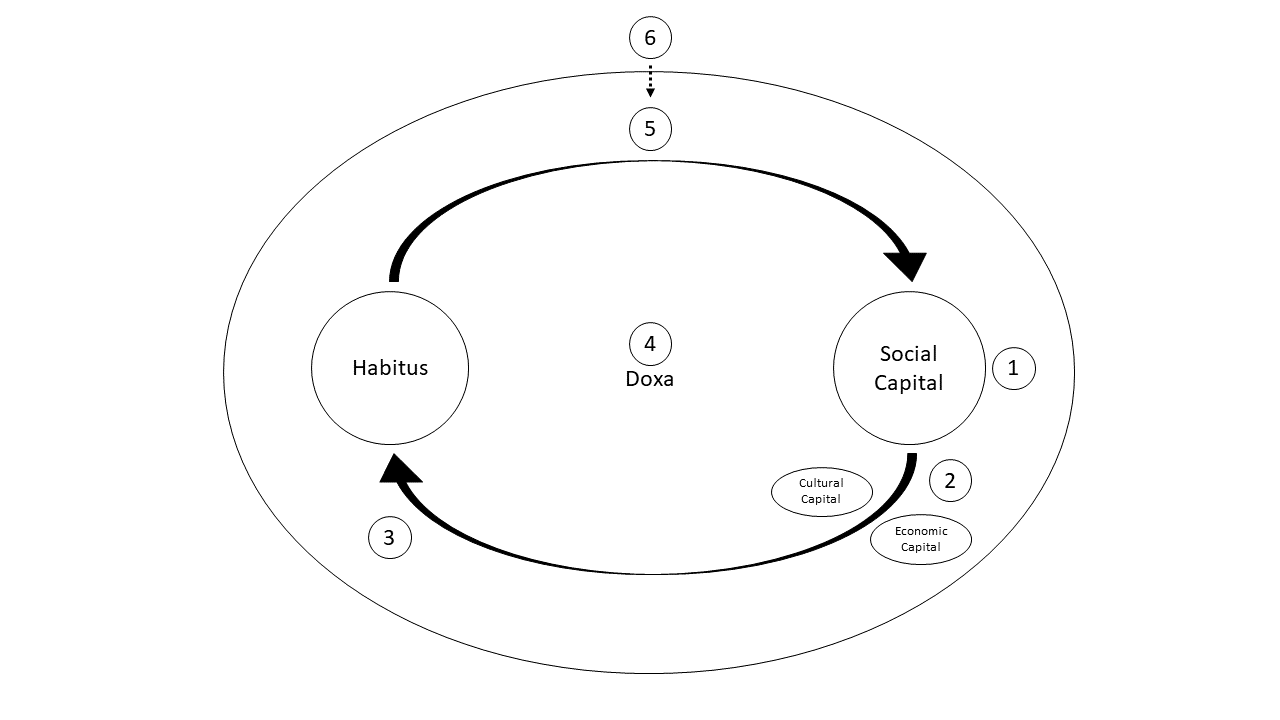
\includegraphics[width=\textwidth]{C5 - Understanding Capital Accumulation/HabitusSocCap_TheoreticalModel.png}
\caption{\label{fig:HabitusSocCap_TheoreticalModel_C6}\textbf{Conceptual Model}. The conceptual model used to understand individual practices in the field of science education. The model, informed by the experiences of participants in the current study, expands on the interaction between habitus and capital originally illustrated by \cite{Bourdieu1984}. The model provides a step by step description of how social capital translates into habitus transformation, and how habitus generates future capital accumulation. Step 1 refers to the initial availability of social capital for an individual. Step 2 refers to the value gained through leveraging social capital into forms of economic and cultural capital. Step 3 refers to how social capital is internalised by the individual. Step 4 refers to how habitus informs the acquisition of future social capital. 5 refers to factors outside of the individual that structure the field (by availability of capital and exchange value).}
\end{figure}

The following sections will describe the perceptions of participants, following the structure of the conceptual model outlined in Chapter 4. While much of my discussion simply describes the experiences that participants reported (semantic themes), the goal of my analysis is to be interpretative \citep{Braun_2006}. This means that I intend to go beneath the level of description and to place participants' experiences into the conceptual model, which I theorize shapes the experiences of participants. Prior research is referenced to support my interpretations. 

\section{Social Capital in the Field of University Science (Step 1)}
This section discusses the availability of social relationships that participants had in the field of university science (Step 1 in Figure \ref{fig:HabitusSocCap_TheoreticalModel_C6}). These relationships are categorised into three key groups, social capital through family connections, social capital through lecturers, and social capital through peers. 

\subsection{Family, Whanau, and Significant Others}
Students' upbringing within the their family and whanau played an important role in students experiences of university science. The M\={a}ori term \textit{whanau} refers to extended family or a community of related families, and therefore this theme refers to the social capital student's held via their parents and siblings, but also through aunties, uncles, and grandparents. Access to social capital through family differed across participants' experiences. Some participants came from highly academic families with science backgrounds, others had whanau with little experience of science education. Following the transition to university study, some participants also had to move away from their family, which could reduce the availability of social capital.

Some participants had family that were interested in science and were available to  talk about it. Some participants remember hearing their parents talking about science from an early age. Susan recalled how her parents discussion of mathematics sparked her interest: ``my parents loved to talk about it. I was very excited when I learned you could do maths at university when I was about 10.''. Even if parent's did not explicitly endeavour to talk to their children about science, having an academic background may enable them to do so. Sean, who's mother worked in a science lab, recalled: \blockquote{I haven't really had much science discussions with my parents, but when the science questions do come up between me and my sister then they sort of hop in.} Many participants recalled their parents holding an interest in science, even if they did not study it at school. Patrick recalled the interactions he would have with his father growing up: \blockquote{My dad used to watch science documentaries all the time just because he found it interesting or whatever. I used to talk to him about stuff like that.}. With that being said, Patrick felt that he did have fewer opportunities to talk about his university degree and plans for the future: \blockquote{most of the time he doesn't know what I’m talking about, but he will still listen to what I’m talking about...  I just have no one to [talk to] really, I don’t ever have to talk to anyone about it. So this is probably the first time.}

In other cases, families were not interested in science. It may be that while a general form of social capital within the family is available, social capital that is valued in the field of university science is not. Chloe recalled that her family, while they valued education, did not value science: \blockquote{my family isn't interested in science and that is cool I am not interested in banking... I think they have no idea of science because they don't do science, so they don't really know what science is so it is kind of like not normal to my family}. Science may not be viewed as something that is interesting for families of students. Aubrey felt that her parents ``switched off'' whenever she tried to talk to them about science: \blockquote{I try to tell them something and they go oh that is nice and just kind of start talking about something else}.

In other cases, family may have a direct negative impact on participants' learning. Some participants found they needed to step away from family, whanau, or significant others who did not value science education in order to aid their educational journey. Renee identified the moment that she left a controlling partner as a key moment in their pursuit of education: \blockquote{It is like when you hold a spring down and it has got so much potential and then you let it go and it is like fuck yeah, do you know what I mean, like that was me leaving that person and being like yeah.}. Leaving a relationship where values regarding education are not shared gave Renee a renewed sense of potential. Hakeem, who argued that ``the priorities are very different for Islanders'' found that moving into his own space allowed him to focus more on his education: \blockquote{...just having that kind of space and gap from your family it was really huge for me.} Previous research suggests that family responsibilities place more demands on Pasifika and M\={a}ori students \citep{zepke2011non}. In a study of post graduate Pasifika university students, \cite{theodore2018pacific} found that family responsibilities were the most commonly cited factor that hindered qualification completion. With that being said, the support of family was the most cited source of help for students, a finding that is reflected in the experiences of participants in the current study (this will be discussed in the following section). 


\subsection{Educators}
The relationships participants shared with their high school teachers, university tutors and lecturers were highly influential in shaping students experiences of university study. Some participants had teachers who were good sources of social capital as they had expertise and knowledge on what was needed to progress to university science. The perceived availability of tutors and lecturers varied from participant to participants, with this being informed by participants' knowledge of how to approach them, and participants' perception of how approachable the educators were. 

The availability of social capital through educators can be driven by students and/or driven by educators. Sean identified that it was his responsibility to approach his teachers when he needed help: \blockquote{All our teachers were way good, so you always had really good teachers and it was just up to you to get what you wanted, just get what you wanted out of them.} With that being said, participants found it easier to make connections with educators when they felt they were approachable. Alicia, who recalled how, even when she did poorly in English, her teacher helped her stay motivated: ``the teacher always encouraged me that you can do well, and I liked her personality and beyond of just studying subject I have more personal attachment to that person.'' The importance of personal attachment was echoed by Stephen: \blockquote{I think the fact that we all could engage in a conversation with him is probably the best thing that a teacher could have}. Belvia found that having lecturer who is friendly and patient made ``a big difference'' to her learning: \blockquote{if someone asked a question in class he would be like oh yeah this is how you do it. He would like draw it out and take his time to actually explain}. Belvia was unable to leverage the same value from a social relationship with another lecturer who did not want to answer her questions straight away: \blockquote{he would just be like go straight onto okay I'll see him later and ask him. I don't know but how can you ask him you are going to forget like I don't know man. It just felt like he did not care.} Belvia's experience demonstrates how the availability of social capital from educators can also be driven by educators themselves. Participants appreciated having teachers who would check in with them and make sure they were on track. Jay recalled how his calculus teacher would ``consistently walk around the class ask if you need help''. Some participants found that educators were more common likely to check in with them in high school, while this was less common at university. 

Some participants found it difficult to approach their high school teachers and lecturers. In some cases this was the result of poor classroom structures that made it difficult to engage with educators. Patrick found that he was not taught much in one of his university classes where lots of students were present: \blockquote{We had a class, a lecture, and most of the lectures were just big tutorials. We weren't taught anything. The teacher would just walk around in a class of about like 80 and we just didn't really learn anything. So we kind of got a bad impression from that class.} 

Educators may also be perceived as intimidating and unapproachable regardless of the classroom structure. These feelings of intimidation may be based on explicit past interactions: ``[the lecturer] definitely did not care because he was like so ruthless. He was like no that is a dumb question.'' (Belivia). Some educators may develop a poor reputation which makes them unapproachable to most students: \blockquote{he used to like not really be rude but give really blunt answers. Yeah so students didn't really ask him much and he kind of has a reputation for being kind of a hard guy.} (Patrick).

In other cases, participants may be unsure about how to approach their educators, even if they did not feel explicitly intimated by them. This may be a particularly salient experience for students after transitioning to university study, where students may sense a change in the rules of the game. Some participants were aware that the rules may be different to high school, and that there may be different conventions to follow when communicating with lecturers or tutors. Paul, a science scholar with mentors at university, did find it difficult to know what conventions to follow:
\blockquote{I haven't emailed anyone, I think about it but again I don't know how I am supposed to approach anyone... I'm never really sure how things work in a university environment, how polite can you be, how do you contact these people in the first place}. In other cases, participants felt that their lecturers could seem ``distant'' (Longolongo).  




\subsection{Peers}
Participants' recalled having different networks of peer relationships open to them. Unlike educators, from which the value of social capital is mainly derived in an academic context, the value of social capital from peers can be both academic and non-academic. While some participants entered into university study with a cohort of students from the same school, other participants entered university with limited peer networks. Students who travel to universities based in different geographic regions from their home town may enter into university with fewer connections. 

The structure of classrooms at high school and university may facilitate or hinder students access to social capital through their peers. 


\section{Leveraging Social Capital (Step 2)}
The value of social capital is derived from the economic and cultural capital that can be mobilised through the connection. These resources may provide students with advantages in supporting their learning and providing student access to information about the field. 

\subsection{Family, Whanau, and Significant Others}
For most students, the family would be the first source of exposure to science. Many participants recalled the different ways that their relationships with their family led to their initial interested in science. Stephen recalled how a space-themed lamp his mother gave him sparked his interest in working for NASA, while Susan points to the significant influence of a book series () in her interest in maths. Regardless of education, having family talk about science could also help spark participants' interest. \blockquote{my mum has bought me books that are like science books or taken books out of the library for me based on science. So I guess that is where I kind of led to go was the fact and she would always tell me if something on the news happened that is very nerdy she would say `oh look at that' and I am like `oh cool' and I would go and research on it.} While Stephen mother did not have a background in science, she was able to elicit enough interest for Stephen to investigate the topic further.

While having family who talk about science is valuable, having conversations with family from educated backgrounds may be especially valuable for students studying at university. Participants may access a flow of information on what is needed to be successful in university and/or science. Sean was introduced to people studying in his field through his iwi: \blockquote{I was just sitting with the adults during some dinner or something and the subject of me would come up somehow and my parents were like oh he wants to be a doctor and they would be like so you need to do this and this and this if you really want to be a doctor}. Some participants acknowledged that talking to their family about their university pathway could be futile if they had not studied in the same area \blockquote{Diana mother}.  Students may also leverage family connections to get employment opportunities, but this is not possible if family connections are not there. Hakeem, who had to amass 800 hours for his engineering degree, described how social connections made it easier for some students: ``It was hard to get the work hours, but also I knew people that did get decent work and they either had connections with their family their dad was an engineer.''


For many participants, simply having the support of their family was viewed as most important to their progression through university. Some participants recalled their parents allowing them to find their own pathway: \blockquote{I think they have always kind of taken the stand that I can sort of dictate where my future goes.} (Lily). For these participants, parents provided everyday support and encouragement, with the main goal for their children to do something that makes them happy. Other participants recalled a more hands-on form of support, where parents would encourage them academically and set expectations for their education. This kind of behaviour can be defined as \textit{concerted cultivation} \citep{lareau2011unequal}, can be more implicit and subtle than overt sources of support from family. Chloe summarised this concept by referring to they way in which she had been ``groomed that you go to university''. Some participants outlined the ways in which parents kept tabs on their academic progress and advocated for them when they felt the school was not meeting expectations. For example, Jay recalled how his mother taught him mathematics at home when she felt that the school teaching him enough.

\subsection{Educators}
Connections with educators offered an important source of support for participants. They were able to answer student's questions on course content, provide advice on study techniques, and give ``insight'' (Susan) on academic pathways. ``he helps me with everything so him being really supportive and really kind it really helps me.'' (Belvia). Students may be most able to leverage the social capital of their teachers were engaging. Participants felt most engaged when teachers provided opportunities for students to be ``hands-on'' (Lucy) in their learning, using experiments instead of just learning from textbooks. \blockquote{jay}.  Participants also enjoyed teachers who provided discussions on real life applications of science. Mark found that his teacher's discussions about science outside of what is being assessed was valuable: \blockquote{He was one of my probably I would say big influences when I came to science. He was a fantastic teacher, really got me into outside of just science as the curriculum. He would really try to show us what I guess the real life things of science were, what you could do in your day to day life, what science meant outside of just what they want you to learn for an exam.} According to \cite{Archer2015a} knowledge on the value of science in future employment is an important form of cultural capital. Participants also valued teachers who had expertise. Hakeem felt that these teachers were most able to reach all students in the classroom: \blockquote{These teachers made sure that the class was interested in what they learned. The way they talked they drew your attention the way they talk and the way they demonstrate things. You could tell they really knew the subjects. If you really know something you can explain it to anyone... that is the key thing for a good teacher, making sure you are able to explain these concepts to different levels of students.}

Participants who felt their teachers were poor recalled having more difficulty in learning.  As summarised by Lucy, having a bad teacher can ``ruin'' a subject, with this resulting in students pursuing different subject disciplines or dropping out of school altogether. Patrick was unable to leverage an advantage with one of his high school teachers as the relationship deteriorated beyond repair: \blockquote{} In contrast to good teachers, participants perceived that poor teachers were less skilled at explaining concepts. Participants ``turned off'' (Kate) when faced with teachers who were confusing, not very ``intriguing'' (Lucy), or did not ``project their passion'' into their teaching (Jay). While good teachers were able to find a balance between controlling the classroom and being approachable, participants did not enjoy classroom experiences when the teacher could not control the class or when the teacher was too strict. 

Some participants entered into university with gaps in their knowledge, which may be attributed to poor experiences in high school or to large differences in the way that university education is structured. Students who feel a tacit ``distance'' (Longolongo) from lecturers or course content may be less able to leverage the advantage of having a teacher. Alicia, who speaks English as a second language, found that psychology was too difficult as it involved a lot of English. Hakeem also recalled having an issue with not understanding what a term meant in one of his mechanics tutorials in his first year: \blockquote{I was like getting stuck on some of the language they were using. Everyone else was like getting into it: `oh yeah we’ll do that', and I was like hold on but they are getting into it they are solving it quickly... It was just a little thing like that. Yeah like I haven’t been brought up in an environment where conversations were had a lot.} Hakeem's experience shows how growing up with exposure to the language used in a field can enable students to engage more with it. Knowing what language or skills are valued in the field is valuable, and utilising this knowledge may increase the chances of success. As described by Longolongo: ``you are not writing for yourself you are writing for them, for their perception''. Longolongo felt it would be better if their lecturer was ``on the same level'' or in the same ``mindset'' as him. 



\subsection{Peers}
For most participants, academic peers were a source of support. This support was utilised explicitly through advice seeking and direct help. Participants saw the benefit of having close peers who they were able to study with. Stephen, who expeirenced a lack of support from one of his teachers, was able to draw upon the support of his classmates to help him: \blockquote{he teaches at a very high level to the point that he only chose specific people to work with, and it kind of got like the other 6 of us or whatever we kind of all fell back. But then we were able to manage to help each other out.}  Through relationships with their friends and academic peers, participants were also able to gain more information on academic pathways, the support groups available to them at university, and what future careers looked like. For example, Mark recalled his resident advisor recommending that he attend lectures for more advanced courses to give him some idea of what the future could hold. Peers could also offer support in a tacit manner, by offering role models for learning, or through vicarious learning experiences (e.g., learning through the questions that peers asked). 

Beyond academic support, participants were grateful for friends that offered them a general, everyday support. Hakeem found that having  consistent For participants who did not have friends who pursued science at university, sharing that knowledge with them could be fulfilling and help ``grow your self-confidence'' (Renee).



\section{Internalising Social Capital (Step 3)}
The social capital that students accrue in university science not only provides access to resources, but it can also influences the way that students see themselves in the field. Capital, which determines students position in the field, is internalised by students via their habitus, which establishes the students disposition towards the field \cite{Bourdieu1992}. Students who hold high levels of social capital may feel an affinity with the field and see progression to university as a ``path already kind of drawn out'' (Chloe), ``inevitable'' (Susan), and those who identified as ``smart'' (Paul) or ``academic'' (Mark) felt like they almost had an obligation to study science. Those who have fewer connections may not feel like the belong, which may be manifested in feelings of not being ``smart enough'' (Patrick), questioning ``should I be here?'' (Renee), or not feeling ``good enough for that space.'' (Hakeem). These feelings can be conflicting, as Longolongo described: ``I feel like I belong in science but I haven’t convinced myself that I belong there''. When asked what it would take to convince Longolongo that he belonged in science, he responded ``I was going to say I need someone to convince me, but no I don’t think so. I think I just have to convince myself''. Longolongo's response brings to light a key aspect of habitus, that while relationships with others are important, we perceive that our convictions are self-directed. The following section expands on how of social relationships with family, educators, and peers are internalised and shape our perceptions of belonging.
 


\subsection{Family, Whanau, and Significant Others}
As outlined by previous theorists \citep{bourdieu1992invitation,Dimaggio1982,Archer_2013,Nash1999} the role of family and whanau extends beyond being a source of social capital. The values and culture espoused by the family are important in molding the internal dispositions that we hold, and the way in which we experience the world around us. As neatly described by Hakeem: \blockquote{You are just shaped purely from who you are with your family.} Having family or whanau who went to university or worked as scientists could signal to students that university science is something they could, or even should, pursue.  Paul felt the pressure of following in his fathers footsteps: ``there are constant reminders, your dad has done all this stuff''. Susan recalled her parents excitement when discussing studying mathematics at university: \blockquote{my parents loved to talk about it. I was very excited when I learned you could do maths at university when I was about 10. So I think it was always going to happen I was going to kind of, I mean it wasn't something I decided then, but I feel like it was inevitable}. 

The pressure that families place on students may set up a feeling of obligation to continue study. Alicia recalled originally enrolling in a commerce degree because ``it was not my choice it is my family choice''. Pressure was not always explicit, with participants referring to parents giving them ``hints'', or feeling ``pushed'' (Diana) towards certain areas of study. These areas of study were mostly related to domains that are widely perceived as prestigious, such as medicine, law, or engineering. Belvia, who was exploring her options at university, recalled her parents' points of view: ``They think science is where you get the money and they just want the whole security stability thing. So they are like science is the better option than like commerce whatever. They would never let me do art, I guess they would but they would be so disappointed.'' In contrast, Chloe's family, who had highly academic backgrounds and ``all work in government education'' did not see science as valuable: \blockquote{I have never ever been able to have an intellectual conversation with them about science, they don't find it interesting... So I am very independent like I don’t really need a sounding board I suppose. Yeah no not really anyone, but that is fine like it doesn't sadden me that I have no one to talk to about science. I know that if I want to talk about science I need to go to someone studying it.} While lack of family interest in science may be a limiting factor for many students, Chloe  demonstrated a resiliency and self-reliance to find sources of social capital outside of her family.

Some participants felt implicitly pressured to continue the social mobility that their parents had underwent. Diana, who was the first in her family to go to university, recalled the expectation her mother put on her: \blockquote{She wanted to go to university but she couldn't because they didn't have enough money or anything. So she kind of worked her way up, a lot of self-taught stuff... she was really pushed me to go to university like no matter what I was doing, she didn't care what I was doing as long as I went to university, but my dad was like you don’t need to go you can just be a tradie}. While Chloe's family did go to university, she recalled ``a big responsibility'' to continue the success of her family: \blockquote{my family are very successful in whatever they do, they all are, so it is expected I don't just be part of the middle working class for the rest of my life I suppose and do something bigger and better}. Belvia felt that one of the main reasons her family emigrated to New Zealand was so that she could attend a good university: ``...coming to New Zealand would be a waste if I didn't even do what my parents wanted me to do''. While the obligation and responsibility felt by students may match up with the students' aspirations, it could also be problematic when students' had other areas of interest. Mark, who's mother in particular viewed him as the ``academic child'' felt a responsibility to study engineering at university: \blockquote{I may have put in my survey how it was [a] sort of pressure when if you are able to do engineering or med... that are looked highly upon by like society or by my family... I could have really enjoyed becoming an English teacher or something because I enjoy that aspect of it, but I guess I am able to do engineering... both literally able to do it and in a more mental academic sense I will get through that}. 

Alternatively, students' parents may prioritise different domains. As mentioned by Hakeem: \blockquote{...[my friends] had tradie dads who made a lot of money going through the ranks of their business and they thought that was the path it was all good.} Hakeem's example elucidates how students may model their aspirations in relation to those they have connections to. Patrick, who had ``heaps of family in the navy'' and went to army cadets, originally aspired to join the army, and ended up working with his father in a saw mill. In contrast, he had no connections to computer science, While Patrick eventually ended up pursuing computer science, he reflected that having connections to people in computer science would have helped:  ``If I just got someone to talk to me [about computer science] when I was young to get me interested in computer science I think that would help.'' 

Lack of family interest in science, or education in general, may provide an environment that signals that science education is not what should be prioritised: \blockquote{The environment I was in, my family, I am an Islander guy, every Islander household I go to, there is no focus whatsoever on education. It is non-existent. They say how is your day going, oh yeah it went all right I got excellence in this - oh cool. But if I made the first 15 rugby I win the game and I get player of the day it's like big celebration big lunch. So the priorities are very different for Islanders so that environment kind of shaped how I was from a young age... There was no kind of push there is no push at all for me to join science [or] engineering.}. Hakeem's story echoes the student experiences recited by \cite{mila2011polycultural}, who points to the difficulties that some Pasifika families can have in transferring Pasifika cultural capital to cultural capital valued by schools. Even when feeling an affinity with science, the prioritisation of sport within his family was difficult for Hakeem to navigate. Hakeem may be viewed as an ``edgewalker'' \citep{krebs1999edgewalkers,tupuola2004pasifika} in that he is someone pioneering new ground and going beyond what is traditionally constituted as Pasifika \cite[p.8]{mila2011polycultural}.  While it is important to note that sport can provide the opportunity for M\={a}ori and Pasifika youth to experience educational success, social position is reinforced when family, teachers, friends hold preconceptions about what forms of education are important to the individual \citep{fitzpatrick2013brown}. In the current study, Chloe commented that parents may be more interested in science if they had more knowledge of how much it applied to their own interests. An awareness of societal inequities facing family, whanau, and people was often a key driver of educational goals. Previous research has also found that giving back to one's community is especially important for indigenous students studying at university \citep{mayeda2014you}.


\subsection{Educators}
Perceptions of educators played an important role in influencing participants identification with a domain. If students perceive that their educators are passionate and excited by the topic they are teaching, it may spread to their students. Many participants recalled feeling inspired to study following a teachers excitement or passion: \blockquote{I always had really good teachers that made me passionate about the subject and I was always seeing their passion kind of made an impact on me as well} (Lucy). Identifying with an educator may also help students identify with a field of study.  Participants were happy if they realised that lecturers were just regular people. As Renee recalled ``seeing there are normal people that just spend their lives doing the things they are passionate about was cool''. The perception of lecturers as ``normal'' people may signify to students that what they do is more realistic and achievable. The sense of belonging students get from their teachers may be especially important if doxa suggests that the student does not represent the typical student in the class. Stephen, who identifies as trans male, felt inspired when he had a lecturer who was also trans: ``[I could] see myself becoming someone like them one day''. For Stephen, exposure to a role model acting out their identity in a position of power signalled to him that his identity was accepted in science : ``it doesn't matter who you are... honestly I look up to her so much because I would not be doing it... I never had someone older than me I could look up to and see myself becoming someone like them one day, and I was like oh finally someone I know I can look up to''. While students who grow up with academics in their family may have more idea as to what lecturers are like and how to engage with them, students who are first in their family to attend university may find it more difficult.

In addition to role modelling, the actions of educators have have significant impacts of students. Participants often appreciated explicitly supportive actions, while feeling \textit{seen} by educators can be a powerful signal. Participants appreciated having teachers who were firm but fair, while students of teachers who were not able to control their classroom or were laisse-fair could develop bad habits. Stephen found that he felt less motivated to work when teachers were more laid back: \blockquote{they are much more chill so I kind of got lagged in my deadlines so I kind of like procrastinated more... and also them being more laid back they didn't really rush to finish everything, and some things I didn't even get taught that were in the exam}. Stephen's example highlights how  Renee detailed one such experience: \blockquote{...he looked at me and did that little like smile thing, like a recognition and I was like that is cool, he remembers the conversation we had and he remembered me} On the other hand, educators who demonstrate poor pedagogy may signal to students that they do not belong. Belvia did not want to engage with her tutors due to unpleasant past experiences: ``sometimes the tutors weren't [very nice], some of them I felt I was dumb asking questions and stuff.'' In experiencing unkindness from those with power, Belvia was felt unwelcome in the field. 



\subsection{Peers}
Participants commonly compared themselves to their friends and classmates, which impacted on the way in which they saw themselves in science and university in general. Participants recalled the way in which their lifestyle was influenced by the norms of their peer groups. This could help develop habits that are valued in educational institutions, as Kate recollected: \blockquote{they called us the angels because we were quite like the goody goods... I started to have more responsible and discipline mind-set not just academics wise but like social wise}. Some participants were more able to share their academic identity with their peers than others. With regards to science, some participants spoke about science with their friends often, while for others discussions of science were limited to university contexts.


Interactions with classroom peers may have influenced how participants viewed themselves in university science. Not fitting in with established structure of the field places extra burden on students. Belvia described her feelings of being the only girl in a computer science test: ``the room was full of guys and they were all like Asian... I was the only girl and I went oh my god... I felt so intimidated, like I am the only girl here I feel like I am going to be so dumb.'' (Belvia). Participants who did not have an established peer network often found that the university tended to be non-social and isolating.

Group work provides one method of reducing feelings of isolation in class, and was viewed positively when it offered students the opportunity to get to know each other. However in other cases it could heighten the pressure to perform. Instead of mitigating the feeling of competition, Chloe felt that groups were often \blockquote{driven by the people who are competitive}. Anxiety could also be heightened when classes required students to change groups regularly. While Hakeem realised his group members were ``not super geniuses'' when he had enough time to get to know them, changing groups regularly made him question himself: ``you are worried about what they are thinking of you and how you perform.'' Stephen recalled needing to ``take a step back'' when he was not comfortable with sharing his identity with new people continually: \blockquote{...the studio physics two hour [tutorial], that kind of scares me because obviously since we get new tables every four weeks only the people that knew me the first four weeks would know I'm trans, and now I've got a whole new set of people and I’m like a bit confronted by them.} For Stephen new groups meant that the chances of being referred to by their dead name were also increased: \blockquote{``it is like a trigger warning to me... I have a rush of anxiety through me} While group work provides an opportunity for students to increase their social connections, requiring students to interact with many different groups serves to benefit students who hold the most capital in the field and who endorse the competitive nature of university science. 

Hakeem felt that the high entry requirements for some fields may engender a sense of competition: \blockquote{the environment kind of like engineering if you got into engineering you should know your shit... I just felt everyone, because the entry was so high, I just felt everyone had to be onto things} Chloe detailed the extent to which competition led to an unwelcoming, and explicitly unfriendly, atmosphere. \blockquote{people just stealing people’s notes or if you left your room unlocked like your laptop would go missing. You could not trust anything at any point} (Chloe). In most cases, the negative impacts of competition were felt implicitly: ``you can just sense it'' (Chloe). 




\section{Doxa (Step 4)}
Outside of the of the social relationships that students hold, general discourses in society influence the development of habitus. 
While feelings of being an ``imposter'' in a domain are often viewed as individualised, private issues, isolated from social contexts, it is important to highlight the pervasive impact that social discourses have on students  \citep{breeze2018imposter}. Bourdieu referred to these general social discourses as doxa, beliefs that are taken as a given. In the current study, participants were well aware of the common societal stereotypes that operate within the field of science. Mark described how even though stereotypes do not make sense, they still inform the world that we see: ``I know that it doesn't make any sense and that is dumb, but then I still kind of from a distance view that''. Participants did offer different suggestions of what a typical scientist looks like, whilst reflecting on how they see themselves in comparison. Many participants depicted scientists as being ``nerdy''. While these points of view may be informed by typically held stereotypes, they may be also realised in their everyday experience. Renee saw stereotypes in her high school science teachers: \blockquote{He was definitely a physicist, like he fitted the part. He wore a suit and a very eccentric tie every day... and he was bald and he had a little physics mono brow going on, you know, that stereotype.} Previous research has shown that discourses referring to scientists as white, male, and nerdy are common \cite{Nosek_2009}, and this doxa may render the field of science as ``unthinkable'' for students who do not match up with them \cite{Archer_2013}. Participants in the current study also tended to view scientists as hard working, smart, and clever --- something that can be ``overwhelming'' (Renee).  Some participants reported a dissonance when comparing these ideals of \textit{smartness} with other aspects of their habitus.

Students from underrepresented groups can face demands to fit their appearance to what is typically accepted in the field of science, which is often perceived as having a ``culture of no culture'' \citep{traweek2009beamtimes}. This perception was shared by Stephen, who saw science as a field where ``it doesn't matter who you are''. However, as argued by \cite{ong2005body}: ``matters of gender, race, ethnicity, social class, immigration status, and sexual orientation have no acknowledged place in this cultureless culture''. While some participants' appearance physically embodied a value of science (e.g., having a science-related tattoo), others felt that their appearance did not conform to the typical rules of their field.  Longolongo recalled the expectations placed on his appearance when he worked as a nurse in Tonga \blockquote{your hair has to be short, you don't wear makeup plus you don't need to have tattoos and nose ring and earrings if you are a male nurse. But I don’t give a damn I still wore my uniform with my tattoos and stuff like that.} Students who do not fit in with the typical, ordinary science student in their field can face additional burdens. Belvia, who saw herself as an extrovert during high school, felt judged for being herself in her computer science class where students were not social: ``I feel like people judge me they are going to be what’s wrong with you. I feel like I have to tone down myself''. These feelings of judgement, being out-of-place, or not belonging can be a significant barrier to learning. 

While \cite{Archer_2013} argue that wider public doxa sees science careers as masculine, it is important to emphasise that discourses operate at the intersection of ethnicity and social class. While science may be viewed as a masculine domain, the expectations for male students from different ethnic groups and/or less affluent backgrounds may be different. While subjects such as computer science may be viewed as a ``guys'' subject (Belvia), participants also commented that male students from lower SES or rural areas tended to be pushed towards vocational careers instead of university. As noted by Stephen: \blockquote{I think [boys] get stereotyped, especially from where I live, they get stereotyped into being a tradie or going for that and not going for the academic route... they should be because they are smart they don't get encouraged}. These stereotypes are particularly salient for young M\={a}ori and Pasifika men. It has been argued that viewing M\={a}ori or Pasifika in terms of their physical attributes reflects a racialised doxa that can limit their potential as learners \citep{hokowhitu2008understanding}. Patrick, who dropped out of high school at 16, found mixed support at school: ``One of my teachers he literally just told me to drop out and start working... that is something a teacher shouldn't be saying''. As outlined by  \cite{hokowhitu2004tackling}, there is a ``hegemonic notion that t\={a}ne should demonstrate their masculinity through physical pursuits such as manual labor and sports.'', and this discourse may inform what is expected for students like Patrick. Patrick also recalled looking for scholarships with his iwi to study science, but found that priority was given for students studying performance arts.  ``a lot of the time you can’t get a scholarship for science degrees through like M\={a}ori tribes... I think we are just expected to do performing arts''

Some female participants in male dominated domains recalled feeling out of place, while M\={a}ori and Pasifika participants experienced dealing with a ``lazy'' stereotype or being ``bubbled'' in a particular way (Chloe): ``you get put into a little bubble that you are going to be lazy, that you are going to drop out of high school, you are not really going to care about your chemistry grades.'' (Chloe). Individuals who represent more than one marginalised group in science may be the subject of ``double jeapody'', where feelings of imposter syndrome are felt even more. As argued by \cite[p.192]{breeze2018imposter}: \blockquote{it does not follow that [feelings of imposterism] are felt equally or that the affect carries the same meaning across discipline, career stage, contract type, and intersections of class, gender, race and ethnicity, sexuality, disability, and factors such as caring responsibilities or first generation in higher education (HE) status.} For example, Patrick, who did not have university educated parents or many other forms of science-related social capital, recalled the way that negative stereotypes regarding M\={a}ori signalled to him that he did not belong at university: \blockquote{...my parents didn't go to uni and growing up... I just thought I wasn't smart enough to go to uni and smart enough to do a science degree... It is just kind of what is drilled into your head when I was growing up} In contrast, Chloe's access to academic cultural capital within her family signalled the opposite: ``being M\={a}ori it was drilled into me that the only way you are going to get ahead in your life is if you have a degree''. The contrasting experiences of Patrick and Chloe highlight the importance of intersectional approaches to understanding student's experiences in science at university. Through this lens, we can see how Chloe's access to academic capital within the family helped transform obstacles into sources of motivation. We can also see the strength that Patrick demonstrated in following his aspirations in the face of societal structures that were stacked against him.

Many resilient participants saw the barriers in their lived experiences as a motivating factor: 
\blockquote{my family have always thought of me when I was younger as a clumsy guy, a clumsy kind of guy who is not very bright... and it has always motivated me to prove to them that I can do things.} (Hakeem).  Developing habitus in opposition to barriers within an individual's field brings to light the extra work that marginalised students take on, but it also should be viewed as a form of capital to be valued. \cite{yosso2005whose}, in a critique of Bourdieu's theory of cultural capital, suggested that the ability to maintain aspirations in the face of barriers (\textit{aspirational capital}) and the knowledge and skills gained through resistance (\textit{resistant capital}) are important forms of cultural wealth. Viewing resilience in the face of barriers as an asset highlights the strength that students can gain from drawing on their own life experiences. With that being said, the chilly climates \citep{Blickenstaff_2005} that marginalised students experience in university science place an unfair burden on students. The competitive environment of university science was an especially salient obstacle to learning commonly touched upon by participants.



\section{Generating Social Capital (Step 5)}
The acquisition of social capital is informed by habitus. 

Students who feel a high level of affinity with education may be more likely to seek out and accumulate social capital, or be more likely to have others form bonds with them. For example, Stephen recalled how two members of his class received more of his teachers time because their parents were also teachers: \blockquote{the two people that he did like they had a lot more knowledge obviously of what they are because they also had parents that are teachers too}. Having knowledge of teachers may have helped these students form a new relationship. Students who are more familiar with university science may be the most likely to view social relationships with those with power as realistic and normal. Some participants would realise the advantages that could be gained by engaging with those with power in the field. Chloe realised her luck at having her chemistry teacher has her form teacher, and made the most of the opportunity: \blockquote{I think you just develop a relationship with your form teacher and therefore I had form time I could ask chemistry questions or I could use that to my advantage}. In contrast, Renee perceived that her form teacher, who was also a calculus teacher, was not interested in helping her: \blockquote{she was one of the teachers that kind of looked at me like the joke student. So she wouldn't have even assumed I would be interested in maths after school. So that topic was never introduced.} In comparing the two experiences of Chloe and Renee, we can see how habitus may relate to the ongoing accumulation of capital. While Chloe was able to leverage an advantage through a social relationship with a receptive teacher, Renee did not have the same opportunity as she assumed the teacher saw her as someone who did not belong. As Renee summarised: \blockquote{I feel like it all depends on if the teacher like believes in you or not, or thinks you are going to amount to something}.

Participants who felt comfortable in the field were happy to find support or talk to lecturers, or happy enough with their position that they felt that they did not need to establish relationships. Susan, a student in the science scholars programme, chose to study in Auckland in part because she felt it would give her more connections: `` just in general I feel from my very limited perspective [Auckland] had better international connections and also science scholars was... influential in my decision... I thought this was the university that would set me up best for going overseas and doing well afterwards''. Even when students did not necessarily know the rules of the game, those with a high affinity with science may be more likely to experience uncomfortable situations in order to build their social capital. For example Paul, who was unsure as to what conventions to follow, saw the benefit in trying: ``I think just trying in the first place, you know, you contact and learn as you go.'' When participants stepped outside of their comfort zone to connect with lecturers, it could have powerful impacts on their academic journey. For example, Renee recalled the moment that she decided to go talk to a senior academic after a lecture had finished: \blockquote{I don't usually like going in front of the whole lecture hall of people down to speak to the lecturer, but the fact that I did have the confidence to do that and the conversation I gained from it literally changed the rest of my uni days, like that is quite significant. That was the defining moment. (Renee)}  Directly following that interaction, Renee made the decision to switch into physics from arts.


For students who feel less affinity with the field, the same relationships may be perceived differently. Hakeem recalled being ``terrified of going to tutorials'', and Belvia was worried about wasting her lecturers time: ``I would be like I can’t waste anyone else’s time. I would be like oh my questions are not worth it.'' When students feel under threat, they may start doubting themselves. \blockquote{Sometimes you start doubting yourself, you ... lose self-confidence. There are so many people... that are doing so much better at it than me, why am I even bothering?} Aubrey fought off her self-doubt by drawing on aspects of her habitus that signalled that the field was where she needed to be: `` I'm like it is not really about other people and what they are doing I guess. So I’m interested in this''.

The power that lecturers hold: ``they are the ones marking our grades and they are the ones who are like the holy grail of knowledge'', may be ``nerve wracking'' and students do not want to risk ``looking dumb'' in front of them (Chloe). Hakeem acknowledged that he could make use of lecturers time more often, but did not want to ``bother''  them: \blockquote{I think it should be something as a student I should get over, you know, go forward and just go talk to them... I should be thinking about really getting to know the lecturers because they obviously have connections and all that would be helpful}. 

In some cases, awareness of competition exacerbated feelings of being an imposter. Some participants recalled feeling intimidated or like they did not belong when they compared themselves to their peers. \blockquote{Sometimes you start doubting yourself, you ... lose self-confidence. There are so many people... that are doing so much better at it than me, why am I even bothering?} (Aubrey). It is important to note that while the culture of academia and science may favour outward expressions of confidence, students may hold their own values that differ from those of the field. For example, some participants made comments relating to being humble in terms of their educational successes. They may feel the need to ``lay low'' or ``not show-off'' (Longolongo), or it may feel ``cocky'' (Hakeem) to identify as being good at science. Humility is particularly valued in M\={a}ori and Pasifika communities, with this reflected in the M\={a}ori concept of \textit{Whakaiti} \cite{haar2018indigenous} and the Tongan concept of \textit{Fakatokilalo} \cite{mafile2004exploring}. 

\section{Institutional Habitus (Step 6)}
The cycle outlined previously can be impacted on by the institutional habitus that dictates how power is distributed in the field. Institutions have the power to offer interventions that may help provide more equitable outcomes for students. Following our conceptual model, these interventions can target different points in the cycle. Interventions may seek to boost the availability of connections for students who enter into university with low levels of social capital, or facilitate students' development of academic identity by combating negative doxa. The relationships shared between and individual and their peers may be improved with well designed group work, while the relationship between lecturers and their students may be improved through the good pedagogy. Through these steps, students may develop a habitus that is more congruent in the domain of science education, and this may aid them in seeking out and forming future relationships in the field. The following chapter will discuss the opportunities for interventions that have helped and may potentially help provide more equitable outcomes in science. 

\section{Conclusion}




\chapter[Opportunities For Interventions][]{Opportunities For Interventions: Making the Field More Equitable}


\section{Introduction}


\begin{figure}[ht]
\centering
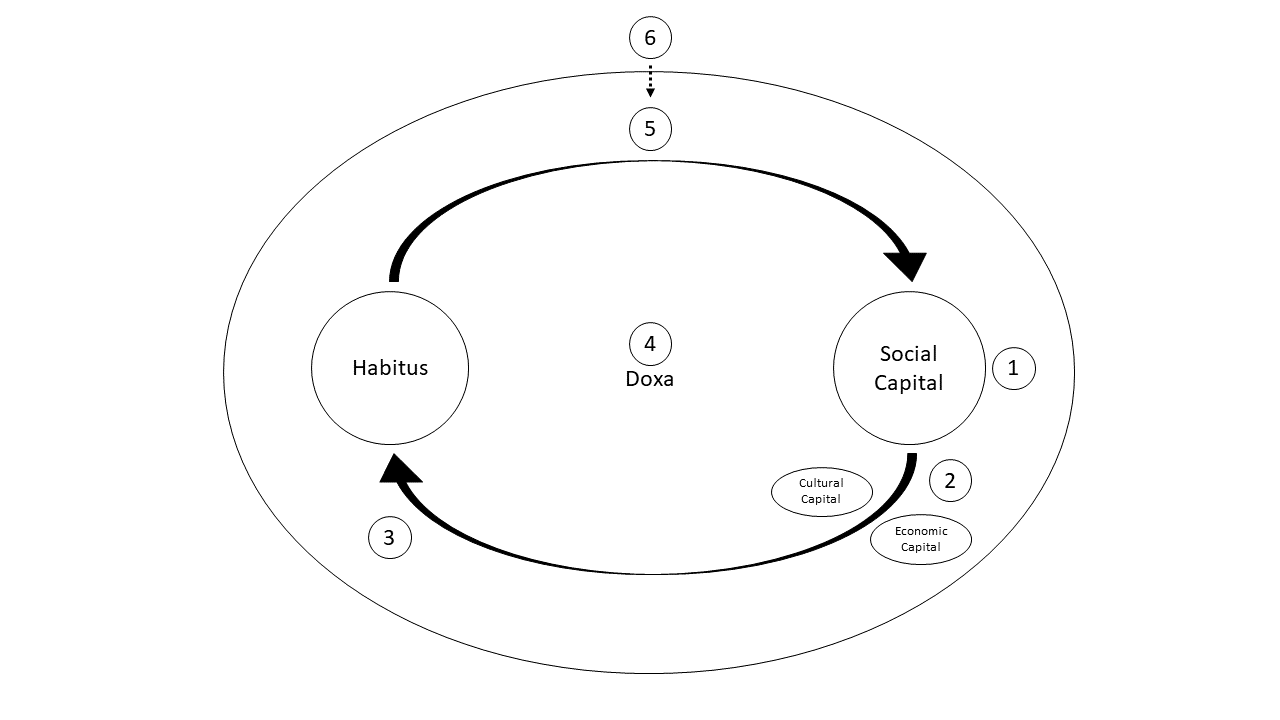
\includegraphics[width=\textwidth]{C5 - Understanding Capital Accumulation/HabitusSocCap_TheoreticalModel.png}
\caption{\label{fig:HabitusSocCap_TheoreticalModel_C7}\textbf{Complete Theoretical Model}. The complete theoretical model. The model, informed by the described experiences of university science students, expands on the interaction between habitus and capital originally illustrated by \cite{Bourdieu1984}. The model provides a step by step description of how social capital translates into habitus transformation, and how habitus generates future capital accumulation. Step 1 refers to the initial availability of social capital for an individual. Step 2 refers to the value gained through leveraging social capital into forms of economic and cultural capital. Step 3 refers to how social capital is internalised by the individual. Step 4 refers to how habitus informs the acquisition of future social capital. 5 refers to factors outside of the individual that structure the field (by availability of capital and exchange value).}
\end{figure}

\section{1: Social Capital in the Field of University Science}
This section discusses the availability of social relationships that participants had in the field of university science. These relationships are categorised into three key groups, social capital through family connections, social capital through lecturers, and social capital through peers. 

\subsection{Direction: Increase Availability of Connections}
It may be possible to address equity issues by increasing the availability of these relationships to students who would not have access to them in their everyday life. Interventions, provided by institutional support services or groups outside of institutions, can mobilise structural changes in the field by increasing the availability of connections. 

For participants in the current study, those who held connections with people who had careers in science (e.g., family members, friends, mentors, lecturers) or experience of university appeared to be the most at home at university. Students who do not have access to these forms of social capital may struggle to envision different careers in science, and what is required to progress in the field. It may be possible to address these issues by increasing the availability of these relationships to students who would not have access to them in their everyday life. As Patrick argued: ``If I just got someone to talk to me when I was young to get me interested in computer science I think that would help.'' (Patrick). Interventions, provided by institutional support services or groups outside of institutions, can mobilise structural changes in the field by increasing the availability of connections. Participants in the current study recalled their own experiences with support groups. For example, Belvia noted how a Women in Computer Science group could aid her in getting her CV out to companies. Many of the participants in the current study gained information about prospective fields through university open days, with this commonly being cited as an important influence in sparking aspirations. 

\section{2: Leveraging Social Capital}
The value of social capital is derived from the economic and cultural capital that can be mobilised through connections with others. These resources may provide students with advantages in supporting their learning and providing student access to information about the field. 


\subsection{Direction: Place Value on Alternative Forms of Cultural Capital}


\section{3: Internalising Capital}
The capital that students accrue in university science not only provides access to resources, but it can also influences the way that students see themselves in the field. Capital, which determines students position in the field, is internalised by students via their habitus, which establishes the students disposition towards the field \cite{Bourdieu1992}. Students who hold high levels of social capital may feel an affinity with the field and see progression to university as a path already drawn out. While some participants found developing relationships with those with power in the field normal, others participants did not make full use of connections as they found it ``nerve-wracking'', their lecturers ``distant'' or intimidating. 


\subsection{Direction: Educator Service Training}
Support services can facilitate students' development of social capital by providing learning environments that are welcoming. This is particularly important in classroom settings, where poor pedagogy can reduce student engagement with course content or cause students to  drop out of courses \cite{russell2011factors}. Efforts to train university teachers can improve student outcomes \cite{gibbs2004impact}, while research from New Zealand suggests that improving the cultural competence of teachers may be especially important for students who are from marginalised groups \cite{ikiua2019pasifika} and/or have English as a second language \cite{campbell2008asian}. Reframing the student-teacher relationship so it is more student-focused \cite{gibbs2004impact} and culturally responsive \cite{ikiua2019pasifika} may reduce the ``distance'' felt by students learning science at university.  




\section{4: Doxa (Societal Discourses)}
Outside of the of the social relationships that students hold, general discourses in society influence the development of habitus.

\subsection{Direction: Provide Counterspaces}


Universities may also seek to serve marginalised students by providing safe, culturally inclusive environments that combat negative doxa. \cite{mayeda2014you} describes how support services offered to M\={a}ori and Pasifika students can act as counter spaces where students can learn in a culturally inclusive environment away from judgement from Pakeha/European peers and teachers. In these spaces, students can experience a learning environment free from doxa. However, as Hakeem recalled, combating the doxa of the field must also be followed with other forms of support: \blockquote{Tu\={a}kana was good but they had the angle of destroying the stereotype for Pacific Islanders, like people normally think you are lazy and all that... it didn't feel that there was much focus on actually living, just getting into uni and getting used to just the basic kind of things, getting used to uni} Beyond combating doxa, support services can provide physical spaces that can help students facilitate connections: \blockquote{The MAPAS students... always hang around the MAPAS house so I just ask those guys. They are always helpful to answer questions from the first years} (Sean). For M\={a}ori and Pasifika students, support services may also provide extra voluntary tutorials that teach in a culturally responsive manner. As Chloe highlighted, Tu\={a}kana offered an environment where ``we all teach one another content or everyone is happy to work with each other...  it is not so cliquey''. Providing this environment can facilitate the formation of social relationships and help develop a supportive group identity. As Lily pointed out: \blockquote{we always sit together as a group during lectures and that and we all support each other through our learning and we help each other out if we don’t understand things, have little study groups. Whereas I’m not sure if the rest of the students in the course feel that way potentially because everyone is competing to get into med. So there is less ability to trust each other as students, but yeah not that same kind of willingness to help between other students}. The social capital that students gain through support services is valuable, not only because it provides academic support, but also because it provides a new norm that runs counter to the culture of independence and competition that is common in university science.

\section{5: Generating Social Capital}
The future acquisition of social capital is informed by habitus.

\subsection{Direction: Reduce the Perceived Power Imbalance}
While students may feel intimated by lecturers due to the power that they wield, counter spaces may also offer students opportunities to engage with them on a more level footing. Patrick found that being a part of Tu\={a}kana open doors: ``the lecturers are really helpful... if you have any questions or anything just go to them and then being part of the Tu\={a}kana programme is really helpful as well people to help you''. As Chloe argued, Tu\={a}kana ``removes that barrier very early'' between lecturers and students. With increased social capital, students have more sources of knowledge on the culture of the fields in which they participate in. This knowledge can inform students perceptions on how they are likely to be treated if they pursue careers in certain fields. These connections can aid students transition to university science by informing them on the content knowledge required to progress in the field. As Lily described, the Hikitia Te Ora course, a preparatory year for M\={a}ori and Pacific students going into first year health science, helped her fill gaps in her knowledge whilst also allowing her to familiarise herself with independent learning that university typically values: \blockquote{I think in terms of confidence it has given me the kind of time to be able to settle myself into some sort of routines and get an idea of what I need, things that I need to think about that I didn't need to when I was staying at home}. 


\section{6: Institutional Habitus}
The cycle is impacted on by interventions operating in the field, which themselves are directed by an institutional habitus.


\subsection{Direction: Equity Charters and Movements}


\section{Conclusion}



\chapter{Summary and Conclusion}


% ====================================================
%
% ENDMATTER
%
% Appendices and bibliography 
% Pagination arabic, re-starts at 1
%
% ====================================================
\cleardoublepage % start afresh on a new page
\setcounter{page}{1} % re-sets the page counter
\appendixpage* % makes a page to mark beginning of appendices
\chapter*{Participant Information}

\section*{Lily}
Lily is a female, second year undergraduate student who identifies as M\={a}ori and P\={a}keh\={a}. She was taking courses in biology, chemistry and physics, and she chose science, not only because she got good grades in it, but also because her family motivated her to take the subject. Lily sees herself as a ``culturally-involved'' person, and she believes this aligns well with her choice to pursue medicine at university as she hopes to help the well-being of her people. Her parents did not attend university, but her father got an education when he worked for the police and regretted dropping out of high school early. While her parents did not put pressure on her to ``go in any certain direction'' or enter into science explicitly, they did want to make sure she was aspiring for something and not just ``settling''. She attended a small, rural high school prior to university study, and took part in the Hikitia Te Ora course, a preparatory year for M\={a}ori and Pacific students going into first year health science. 

\section*{Renee}
Renee is a female, second year undergraduate student who identifies as P\={a}keh\={a}. She attended a public, rural single sex girls school, and has always wanted to be in the police. She is studying physics at university just because she is interested in the subject and sees herself as a naturally curious person. She was originally enrolled in an arts degree but switched to a conjoint with physics after being inspired by a senior physics lecturer. While a high achiever, she felt that people saw her as a ``joke student'' and did not expect her to go on to university study. Renee is the first in her family to attend university, and does not have family who work as a scientist or in a job that uses science. She  and loves sharing knowledge with her friends and family: ``I can't talk to my parents and be like why does this work because they don't know. So I'm like if I can figure it out for myself and gain the knowledge myself then that's cool. Teach my kids one day and maybe make them more interested in the world.''

\section*{Belvia}
Belvia is a female, fourth year undergraduate student who identifies as Indian. Belvia's family emmigrated to New Zealand from India when she was 9 years old. Belvia says that her parents, who both went to university, were motivated to come to New Zealand to provide their children with access to university study. Belvia felt a lot of pressure from her parents to perform well academically and study at university. originally intended to study engineering, but did not meet the entry requirements. She changed her major to commerce, but after two weeks decided that was not for her. Belvia then went in to computer science following the recommendation of a ``friend of a friend'', but went into the degree not knowing much about what was involved: ``I didn’t know anyone who did this degree and I was so confused... I was so confused in first year I was oh what is happening.'' Prior to university, Belvia attended a small, single sex private school, in part because her father was worried about ``drugs and stuff'' in public school. Belvia enjoyed her time at her high school, which she felt was ``like a second family''. She recalled being an extrovert at high school when she was surrounded by her friends, but feels ``isolated'' at university where students keep to themselves. She is unsure of what ``kind of person'' (``I don’t view myself as an art person, I don't view myself as a maths person'') she is, but feels that this will come once she has graduated and got a job that she likes.


\section*{Chloe}
Chloe is a female, second year undergaduate student who identifies as M\={a}ori. She comes from a highly academic family, with three generations of her family attending university. She spent an extended period in the hospital while she was young, and decided that she wanted to work as a doctor, which her parents ``supported that times a hundred.'' While she also wanted to be a dancer, that goal was ``crushed'' with the expectation that she would go to university. She has a passion for mental health and aspires to be a clinical psychologist. She originally pursued biomed and health at a different university, but changed her path after experiencing an unhealthy competitive culture. She is part of a ``very strong minded successful M\={a}ori family'', who have expectations for Chloe to continue to break the cycle of oppression. She is now studying psychology, which she feels is ``not sufficing'' with regards to her own and her family's expectations,as it is a ``generic'' degree. Chloe feels she is expected to go overseas to complete post-graduate qualifications, maybe at an ivy league institution. Chloe feels a ``big responsibility'' to live up to her family's expectation and continue ``to make a positive influence in M\={a}ori society''.


\section*{Lucy}
Lucy is a female first year undergraduate student who identifies as P\={a}keh\={a}. Lucy spent most of her life in Switzerland, but her parents lived in New Zealand for an extended time before Lucy was born. Both of Lucy's parents are professionals who work in science. She has wanted to study physics since she was young: ``I told my parents when I was seven that I wanted to be a physicist and I always stuck to it''. Her current ``dream goal'' is to become a sailor, and this influenced her to continue to study physics with exercise science. Lucy attended a prestigious private school prior to university where she gained an IB qualification. 

\section*{Sean}
Sean is a male first year undergraduate student who identifies as M\={a}ori and Nieuen. He attended a public, single-sex boys school in Auckland prior to university. Sean is studying courses in biology and chemistry, with the goal of becoming a surgeon. His aspirations are tied to his religious views, where he is encouraged to be ``more Christ-like'', and his cultural identity. He sees things like heart disease as a major concern for M\={a}ori and Pacific populations: ``maybe being able to help people out with heart disease would be a good thing, but support to help my family out''. Prior to university, he undertook a mission with his church which helped him develop self-discipline. Sean's mother has a science degree, while his sister just graduated with a science degree in biomed and is undertaking postgraduate study. Sean's parents always expected him to do well in school, but made sure he had experiences of doing non-academic jobs, such as working in a factory. 

\section*{Mark}
Mark is a first year undergraduate student who identifies as P\={a}keh\={a} and M\={a}ori. He attended a private school where he underwent CIE qualifications and achieved a maximum rank score. At his high school, Mark felt that ``it was sort of like an assumption that everyone was going to uni ''. Mark is now studying engineering at university, although he is unsure of what being an engineer actually looks like. He commented that he could have enjoyed being an English teacher, but he felt pressure to do engineering because he is ``literally able to do it and in a more mental academic sense I will get through''. Marks's father, who did a pharmaceutical degree at university, advised Mark to not go into pharmacy because he felt it is boring, but to do something that he enjoyed. Mark did recall pressure from his Mum, who holds expectations for Mark being the ``academic child''. Mark felt that he does not really fit the typical stereotype of a scientist both appearance wise (``I don’t fit the whole archetype of like nerdy engineering kid'') and when he compares himself to some of his friends who are ``really studious''. With that being said, Mark ran the after school science club for his school, and is passionate about science. 


\section*{Jay}
Jay is a male, first year undergraduate who identifies as European. He is originally from South Africa, and moved to New Zealand when he was 9 years old. He is now studying computer science with the goal of working in a mix of finance and computers. Both of Jay's parents went to university, with Jay's father completing two degrees in electrical engineering and computer science. While Jay's parents ensured that Jay progressed academically by teaching him outside of school hours, they had the ``philosophy that whatever you want to do to make you happy would be the best to do''. Prior to university, Jay attended a high school with no designated curriculum, but switched to a public school after him and his parents decided that it was not a good fit. 

\section*{Alicia}
Alicia is a female, first year undergraduate student who identifies as Chinese. She went to high school and completed a degree in commerce in China before moving to New Zealand to study computer science as a mature student. She did not like commerce, and stated that it was a ``family choice''. As Alicia is the first in her family to attend university, she says that this choice was informed mainly by stereotypes held by her family (``girls need to do girls job''). Even though her parents did not attend university, Alicia found that the her parents gave her an environment that facilitated her interest in science. While she has a good relationship with her mother, she left China in part to ``run away'' from family pressure and a working culture that competitive and ``not that friendly to women''. Alicia decided to study computer science at university in New Zealand after working with an IT company and being ``immersed'' in that environment. She feels that computer science aligns with her ability to problem solve, and aspires to be a data scientist working in silicon valley.


\section*{Aubrey}
Aubrey is a female, third year undergraduate student who identifies as P\={a}keh\={a} and M\={a}ori. She is studying biology and is the first in her family to attend university. While she sees herself as an ``artsy'' person, she has always been interested in science. She attributes the start of this interest to science books she read when she was around 9 years old. She went to a school ``a poor area'', and did not think she ``would get into university''. She enjoyed science at high school and recalls having teachers who were enthusiastic and excited about teaching, and felt they expected her to go on to university. After high school, Aubrey ended up in Auckland after her mother found her a administration job. Aubrey found that this job ``is really not for me'' and wanted something that was more stimulating. She chose to study biology at university as she did not do as well in chemistry, and did not know what jobs were available in physics. She would like to work in forestry science: ``I just love trees and I grew up around forestry''. Aubrey feels she is quite shy, and would struggle to talk to her lecturers: ``I’m just nervous I don’t know how to approach anyone about that''. Her parents are both employed in the social work space, but Aubrey feels like that would not be ``very fulfilling'' for her. She is more motivated to help solve environmental issues. While she was one of only a few students from her school who went to study science at university, Aubrey is able to talk to her friends and her partner about what she studies. She is thankful for the support she received from her family, friends and teachers. 


\section*{Stephen}
Stephen is a trans male, first year undergraduate student who identifies as P\={a}keh\={a} and M\={a}ori. He is studying physics, and he has always wanted to work for NASA (aspiring to be a rocket physicist or chemist). This may have been informed by Stephen's mother (who went to university, but not in science) talking about the moon-landings and space while he was growing up. He feels a high level of affinity with science, and feels that his friends see him as a ``nerd'': `` everyone is like oh you are such a nerd and I’m like yeah that's me''. Prior to university, Stephen attended a private school and then moved to a public rural school for his last two years of high school. He found that private school ``spoon-feeds'' students to go to university, while most of his peers at rural school went into vocational careers. Stephen has found the transition to university study difficult as he misses rural life, and few of his friends from high school moved to Auckland. Stephen has also had to navigate discussing his gender identity with his new peers, and this can be anxiety provoking: ``it is like quite confronting and nerve wracking for me to open up to people about me''. With that being said, Stephen is proud of himself for making new friends, and he feels ``blessed'' to have friends and teachers who support him and his identity.  

\section*{Hakeem}
Hakeem is a male, fourth year undergraduate student who identifies as P\={a}keh\={a} and Tongan. He is now studying computer science, after switching from his original engineering degree. This swap was motivated partly because he felt ``naturally better'' at the software side of engineering than the hardware side, and partly because he was worried he would not get enough work hours to complete his engineering degree (engineering students are required to complete 800 hours work experience). Hakeem found that many engineering students are able to attain hours due to family connections in the field, which he does not have. Hakeem's parents did not attend university, and they did not get involved in his academic life. Hakeem, who also played rugby to a high standard, felt like his family were more interested in his sporting achievements than his academic ones: ``I felt like during high school especially I wasn't guided at all by anyone really. My parents were non-existent in my high school life they didn't really put any attention towards where I was going''. He went into the first year of engineering as ``one of the only Islanders in the class'' and sometimes felt anxious and under pressure to perform. After experiencing adversity in his family life, he moved into his own place with his girlfriend and is feeling ``happier and more content''. He attributes much of his current motivation and success to wanted to provide for his girlfriend, while he also acknowledges the importance of having ``consistent'' friends, and ``very good'' high school teachers. Hakeem wants to work as a data scientist, and is intrinsically motivated to succeed: ``I'm self-aware of how much I enjoy it and that is why I kind of do it''.  

\section*{Patrick}
Patrick is a male, second year undergraduate student who identifies as M\={a}ori. He attended a single sex boys school, but dropped out of high school when he was 16 years old. He received mixed support at high school with one teacher telling him he should drop out, but with the dean trying to encourage him to stay. He originally intended to join the army, following in the steps of much of his family, but ended up working in a saw mill with his father. He draws upon this experience as a prime motivator for why he went to university: ``it was a really hard job and I hated it. So that is probably why I ended up coming to uni.'' He is now studying computer science as he likes technology and feels there is good opportunity to earn money. Patrick's parents did not go to university, but he talks with his Dad about science and his degree. Patrick sees stereotypes facing M\={a}ori as a motivating factor: ``that is kind of the reason why I want to study science as well because a lot of people think oh you are Maori, you are Polynesian, you are not smart enough to do stuff like that.'' He has found teachers at university ``way more helpful'' than those at his high school, and spends much of his university days at Tu\={a}kana, a university support service for M\={a}ori and Pasifika students.  

\section*{Longolongo}
Longolongo  is a male, third year undergraduate who identifies as Tongan. He attended high school in Tonga, and worked as a nurse prior to attending university, where he is studying biology. Longolongo wants to ``make a mark back in Tonga'' and has aspirations to set up a forensics department. Longolongo described himself as a ``a bit like weird twink'', who many people in Tonga find rebellious. He encountered opposition to his lifestyle while growing up in Tonga and working as a nurse but he stayed true to himself. Longolongo's parents did not attend high school or university, but they gave him support to be himself in his everyday life: ``I was the only fem boy back in our village and my parents usually like don’t give a f like how I behave and stuff like that... They didn't want me to kind of like not follow myself I think, and back in Tonga people usually listen to others but my parents they didn't.'' Longolongo found the transition to and English speaking university difficult, and feels that given the high tuition he has to pay, there should be more support. 


\section*{Diana}
Diana is female, first year undergraduate student who identifies as P\={a}keh\={a}. She is in her first year of studying chemistry at Auckland, while she is also enrolled in a diploma of languages. Diana spent the previous year studying geology in Wellington, but decided to change her degree as geology was not ``for her'' and she did not find it interesting. She originally chose geology as she thought it had good job prospects, paid well, and was easy (``okay geology how hard can it be''). Diana is the first in her family to attend university, her father works as a ``tradie'' and her mother works in IT. Diana recalled feeling ``pushed'' by her mother in particular to go into IT. She went to a single-sex girls school, where she felt that her teachers she felt like her teachers did not recognise her as being good at science, but saw her as ``kind of like the dumb one of the smart girls, or like the smart one of the other students''. 





 

%\printbibliography[title={Works cited}, heading=bibintoc]
\bibliography{bibfile.bib}
\bibliographystyle{apalike}       % APA-like style


\end{document}